\documentclass[letterpaper,10pt,headsepline]{scrbook}
\usepackage[T1]{fontenc} 
\usepackage{natbib}
\usepackage{supertabular}
\usepackage{epsfig}
\usepackage{ifthen}
\usepackage{index}
\usepackage[backref,colorlinks]{hyperref}
\usepackage{listings}
\usepackage{verbatim}
\usepackage{hyphenat}
\usepackage{ragged2e}
\usepackage[acronym]{glossaries}
\usepackage{color}
\usepackage{tensor}
\usepackage{textcomp}
\usepackage{amssymb}
\usepackage{amsmath}
\usepackage{bm}

% Adaptive labelling.
\makeatletter
\newcommand{\iflabelexists}[3]{\@ifundefined{r@#1}{#3}{#2}}
\makeatother

% Table of contents
\setcounter{tocdepth}{5}

% Margins.
\setlength{\topmargin}{0mm}
\setlength{\textwidth}{160mm}
\setlength{\textheight}{210mm}
\setlength{\oddsidemargin}{0mm}
\setlength{\evensidemargin}{0mm}

% Useful commands.
% Names
\def\glc{{\normalfont \scshape Galacticus}}

% Physical constants.
\def\G{\mathrm{G}}
\def\clight{\mathrm{c}}
\def\d{\mathrm{d}}
\def\e{\mathrm{e}}

% Variable specifiers.
\def\void{\textcolor{red}{\textless void\textgreater}}
\def\logicalzero{\textcolor{red}{\textless logical\textgreater}}
\def\logicalone{\textcolor{red}{\textless logical(:)\textgreater}}
\def\logicaltwo{\textcolor{red}{\textless logical(:,:)\textgreater}}
\def\intzero{\textcolor{red}{\textless integer\textgreater}}
\def\intone{\textcolor{red}{\textless integer(:)\textgreater}}
\def\inttwo{\textcolor{red}{\textless integer(:,:)\textgreater}}
\def\intthree{\textcolor{red}{\textless integer(:,:,:)\textgreater}}
\def\doublezero{\textcolor{red}{\textless double\textgreater}}
\def\doubleone{\textcolor{red}{\textless double(:)\textgreater}}
\def\doubletwo{\textcolor{red}{\textless double(:,:)\textgreater}}
\def\doublethree{\textcolor{red}{\textless double(:,:,:)\textgreater}}
\def\enum{\textcolor{red}{\textless enumeration\textgreater}}
\def\argin{\textcolor{blue}{$\rightarrow$}}
\def\arginout{\textcolor{blue}{$\leftrightarrow$}}
\def\argout{\textcolor{blue}{$\leftarrow$}}

% Macros for linking to sections either through internal LaTeX label/ref or externally through hyperdef/hyperref.
%% Link to a class by class name.
\newcommand{\refClass}[1]{\ifthenelse{\equal{\docname}{Development}}{{\normalfont \ttfamily #1} (see \S\ref{class:#1})}{\href{https://github.com/galacticusorg/galacticus/releases/download/bleeding-edge/Galacticus_Development.pdf\#class.#1}{\normalfont \ttfamily #1}}}
%% Link to a physics description by class name.
\newcommand{\refPhysics}[1]{\ifthenelse{\equal{\docname}{Physics}}{{\normalfont \ttfamily #1} (see \S\ref{phys:#1})}{\href{https://github.com/galacticusorg/galacticus/releases/download/bleeding-edge/Galacticus_Physics.pdf\#physics.#1}{\normalfont \ttfamily #1}}}


% Build glossary and index.
\makeglossary
\glstoctrue
\makeindex

% Acronyms.
\newacronym{cdm}{CDM}{cold dark matter}
\newacronym{cmb}{CMB}{cosmic microwave background}
\newacronym{igm}{IGM}{intergalactic medium}
\newacronym{imf}{IMF}{initial mass function}
\newacronym{isco}{ISCO}{innermost stable circular orbit}
\newacronym{ism}{ISM}{interstellar medium}
\newacronym{ode}{ODE}{ordinary differential equation}
\newacronym{nfw}{NFW}{Navarro-Frenk-White (dark matter halo profile)}
\newacronym{sed}{SED}{spectral energy distribution}
\newacronym{sne}{SNe}{supernovae}
\newglossaryentry{adaf}{type=\acronymtype, name={ADAF}, description=\glslink{adafg}{advection-dominated accretion flow}, first={advection-dominated accretion flow (ADAF)}, see=[Glossary:]{adafg}}
\newglossaryentry{pah}{type=\acronymtype, name={PAH}, description=\glslink{pahg}{polycyclic aromatic hydrocarbon}, first={polycyclic aromatic hydrocarbon (PAH)}, see=[Glossary:]{pahg}, firstplural={polycyclic aromatic hydrocarbons (PAH)}, see=[Glossary:]{pahg}}
\newglossaryentry{dsl}{type=\acronymtype, name={DSL}, description=\glslink{dslg}{domain-specific language}, first={domain specific language (DSL)}, see=[Glossary:]{dslg}, firstplural={domain-specific languages (DSLs)}, see=[Glossary:]{dslg}}
\newacronym{sdss}{SDSS}{Sloan Digitial Sky Survey}
\newglossaryentry{ahf}{type=\acronymtype, name={AHF}, description=\glslink{ahfg}{Amiga's Halo Finder}, first={Amiga's Halo Finder (AHF)}, see=[Glossary:]{ahfg}}
\newacronym{mcmc}{MCMC}{Markov Chain Monte Carlo}
\newglossaryentry{sam}{type=\acronymtype, name={SAM}, description=\glslink{samg}{semi-analytic model}, first={semi-analytic model (SAM)}, see=[Glossary:]{samg}, firstplural={semi-analytic models (SAMs)}, see=[Glossary:]{samg}}
\newglossaryentry{bie}{type=\acronymtype, name={BIE}, description=\glslink{bieg}{semi-analytic model}, first={Bayesian inference engine (BIE)}, see=[Glossary:]{bieg}, firstplural={Bayesian inference engines (BIEs)}, see=[Glossary:]{bieg}}
\newglossaryentry{hod}{type=\acronymtype, name={HOD}, description=\glslink{hodg}{halo occupation distribution}, first={halo occupation distribution (HOD)}, see=[Glossary:]{hodg}, firstplural={halo occupation distributions (HODs)}, see=[Glossary:]{hodg}}
\newglossaryentry{mpi}{type=\acronymtype, name={MPI}, description=\glslink{mpig}{message passing interface}, first={message passing interface (MPI)}, see=[Glossary:]{mpig}, firstplural={message passing interfaces (MPIs)}, see=[Glossary:]{mpig}}
\newglossaryentry{pbs}{type=\acronymtype, name={PBS}, description=\glslink{pbsg}{portable batch system}, first={portable batch system (PBS)}, see=[Glossary:]{pbsg}, firstplural={portable batch systems (PBSs)}, see=[Glossary:]{pbsg}}

% Glossary entries.
\newglossaryentry{component}{name={component}, description={An individual physical system within a \gls{node}, such as a dark matter halo, a galactic disk or a supermassive black hole}}

\newglossaryentry{forest}{name={forest}, description={A collection of merger trees that are linked together by virtue of nodes which jump between trees}}

\newglossaryentry{node}{name={node}, description={A single point in a merger tree, consisting of a dark matter halo and associated baryons}}

\newglossaryentry{mergee}{name={mergee}, description={For a given node in a merger tree, the set of mergee nodes consists of all nodes which will undergo a galaxy merger with the node at some point in the future}}

\newglossaryentry{primary progenitor}{name={primary progenitor}, description={The progenitor of a given \gls{node} which is regarding as the direct descendent of that \gls{node} (often, but not always, the most massive progenitor). Other progenitors are considered to merge into this primary progenitor}}

\newglossaryentry{parent}{name={parent}, description={In a merger tree, the parent node of any given node that exists at time $t_0$ is that node to which it is directly connected in the tree at time $t_1>t_0$}}

\newglossaryentry{Bernoulli distribution}{name={Bernoulli distribution}, description={A discrete probability distribution which takes value $1$ with success probability $p$ and value $0$ with failure probability $q = 1-p$. Read more on \href{http://en.wikipedia.org/wiki/Bernoulli_distribution}{Wikipedia}}}

\newglossaryentry{UUID}{name={UUID}, description={A \href{http://en.wikipedia.org/wiki/Universally_unique_identifier}{universally unique identifier}---this is a label which uniquely identifies some object (in this case, a \glc\ model)}}

\newglossaryentry{ABmagnitude}{name={AB magnitude}, description={An astronomical magnitude system in which the apparent magnitude is defined as $m=-2.5\log_{10}f-48.60$ for a flux density, $f$, measured in ergs per second per square centimeter per hertz}}

\newglossaryentry{forwardDescendent}{name={forward descendent}, description={The node with which the mass (or majority of the mass) of a node will become associated with at a later time. This type of descendent is usually relevant when considering how halos and galaxies evolve forward in time and should be distinguished from a \gls{backwardDescendent} which is relevant when building merger trees}}

\newglossaryentry{backwardDescendent}{name={backward descendent}, description={The \gls{primary progenitor} of a node. This type of descendent is usually relevant when building merger trees and should be distinguished from a \gls{forwardDescendent} which is relevant when considering how halos and galaxies evolve forward in time}}

\newglossaryentry{MD5hash}{name={MD5 hash}, description={The \href{http://en.wikipedia.org/wiki/MD5}{MD5 Message-Digest Algorithm} is a widely used cryptographic hash function that produces a 128-bit (16-byte) hash value. In \glc\ it is used to encode unique labels for modules which are incorporated into file names. \glc\ uses the \href{http://www.gnu.org/software/libc/}{\tt glibc} \href{http://en.wikipedia.org/wiki/Crypt_(Unix)}{\tt crypt()} function to compute MD5 hashes, but switches ``{\tt /}'' for ``{\tt @}'' in the hash (since ``{\tt /}'' is inconvenient for use in file names)}}

\newglossaryentry{LymanContinuum}{name={Lyman continuum}, description={The part of the electromagnetic spectrum which is capable of ionizing hydrogen, i.e. photons with wavelengths shorter than 91.1267~nanometres and with energy above 13.6~eV}}

\newglossaryentry{millenniumSimulation}{name={Millennium Simulation}, description={The \href{http://www.mpa-garching.mpg.de/galform/virgo/millennium/}{Millennium Simulation} is a high-resolution N-body simulation of structure formation in a cold dark matter universe.}}

\newglossaryentry{latinhypercube}{name={Latin hypercube}, description={A \href{http://en.wikipedia.org/wiki/Latin_hypercube_sampling}{Latin hypercube} is a construct for generating a sample of plausible collections of parameter values from a multidimensional distribution}}

\newglossaryentry{maximin}{name={maximin}, description={In \gls{latinhypercube} design, the ``maximin'' approach generates a large number of \glspl{latinhypercube} and selects the one which has the greatest minimum distance between all pairs of points in the hypercube}}

\newglossaryentry{adafg}{name={ADAF},
    description={An advection-dominated accretion flow (ADAF) is a particular solution for an accretion flow around a black hole, star or compact object in which energy liberated by viscous forces is stored within the accretion flow and advected inward to the central object (see \citealt{narayan_advection-dominated_1998})}}

\newglossaryentry{pahg}{name={PAH},
    description={\href{http://en.wikipedia.org/wiki/Polycyclic_aromatic_hydrocarbon}{Polycyclic aromatic hydrocarbons} (PAH) are large organic molecules consisting of fused aromatic rings}}

\newglossaryentry{dslg}{name={DSL},
    description={\href{http://en.wikipedia.org/wiki/Domain-specific_language}{Domain-specific languages} (DSL) are a type of programming language dedicated to a particular problem. In \glc\ a DSL is used to specify the structure of \glspl{component}}}

\newglossaryentry{samg}{name={SAM},
    description={Semi-analytic models (SAMs) are a type of galaxy formation model utilizing simple parameterizations of physical processes to follow the evolution of galaxies through a merging hierarchy of galaxies.}}

\newglossaryentry{ahfg}{name={AHF},
    description={\href{http://popia.ft.uam.es/AHF/files/AHF.pdf}{Amiga's Halo Finder} (AHF) is a software package which identifies dark matter halos in N-body simulations. Full details are given by \cite{gill_evolution_2004} and \cite{knollmann_ahf:_2009}}}

\newglossaryentry{hodg}{name={HOD},
    description={A halo occupation distribution (HOD) is a mathematical model describing the distribution of the number of galaxies (of some given physical properties) found in a dark matter halo of given mass.}}

\newglossaryentry{bieg}{name={BIE},
    description={The \href{http://www.astro.umass.edu/BIE/}{Bayesian Inference Engine} (BIE) is a software package designed to facilitate exploration of complexes parameter spaces using Bayesian techniques.}}

\newglossaryentry{mpig}{name={MPI},
    description={\href{http://en.wikipedia.org/wiki/Message_Passing_Interface}{Message Passing Interface} (MPI) is a standard for passing messages between processes on parallel computers.}}

\newglossaryentry{pbsg}{name={PBS},
    description={\href{http://en.wikipedia.org/wiki/Portable_Batch_System}{Portable Batch System} (PBS) is a job scheduler used on many compute cluster environments.}}


\begin{document}

\lstset{language=[95]Fortran}

\frontmatter

\pagestyle{empty}
\begin{center}
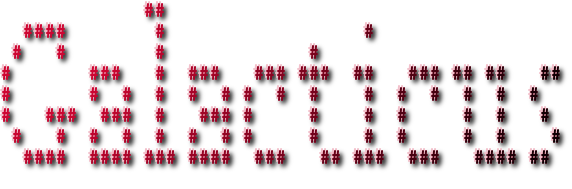
\includegraphics[width=125mm]{GalacticusLogo.png}\\

\Huge Installing and Using \normalsize

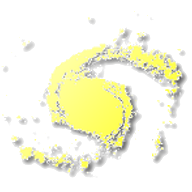
\includegraphics{New_Logo_Galaxy_192_Transparent.png}\\
A semi-analytic galaxy formation code.\\

\copyright\ 2009, 2010 2011, 2012, 2013, 2014, 2015, 2016, 2017, 2018, 2019, 2020 Andrew Benson
\end{center}

\tableofcontents

\mainmatter
\pagestyle{headings}


\chapter{About Galacticus}

\glc\ is a semi-analytic model of galaxy formation. It solves equations describing how galaxies evolve in a merging hierarchy of dark matter halos in a cold dark matter universe. \glc\ has much in common with other semi-analytic models, such as the range of physical processes included and the type of quantities that it can predict.

In designing \glc\ our main goal was to make the code flexible, modular and easily extensible. Much greater priority was placed on making the code easy to use and modify than on making it fast. We believe that a modular and extensible nature is crucial as galaxy formation is an evolving science. In particular, key design features are:
\begin{description}
 \item [Extensible methods for all functions:] Essentially all functions within \glc\ are designed to be extensible, meaning that you can write your own version and insert it into \glc\ easily. For example, suppose you want to use an improved functional form for the \gls{cdm} halo mass function. You would simply write a subroutine conforming to a specified template that computes this mass function and add a short directive (see \S\ref{sec:CodeDirectives}) in your code which explains to the build system how to insert this function in \glc. A recompile of the code will then incorporate your new function.

 \item [Extensible components for tree nodes:] The basic structure in \glc\ is a merger tree, which consists of a linked tree of nodes which have various properties. \glc\ works by evolving the nodes forwards in time subject to a collection of differential equations and other rules. Each node can contains an arbitrary number of \emph{components}. A component may be a dark matter halo, a galactic disk, a black hole etc. Each component may have an arbitrary number of \emph{properties} (some of which may be evolving, others of which can be fixed). \glc\ makes it easy to add additional components. For example, suppose you wanted to add a ``stellar halo'' components (consisting of stars stripped from satellite galaxies). To do this, you would write a module which specifies the following for this component:
 \begin{itemize}
  \item Number of properties;
  \item Interfaces to set and get property values and rates of change;
  \item ``Pipes'' which allow for flows of mass/energy/etc. from one component to another;
  \item Functions describing the differential equations which govern the evolution of the properties;
  \item Functions describing how the component responds to various events (e.g. the node becoming a satellite, a galaxy-galaxy merger, etc.);
  \item Auxiliary functions for handling outputs etc.
 \end{itemize}
 Short directives embedded in this module explain to the \glc\ build system how to incorporate the new component. A recompile will then build your new component into \glc. Typically, a new component can be created quickly by copying an existing one and modifying it as necessary. Furthermore, multiple implementations of a component are allowed. For example, \glc\ contains a component which is a Hernquist spheroid. You could add a de Vaucouler's spheroid component. A simple input parameter then allows you to select which implementation will be used in a given run.

 \item [Centralized ODE solver:] \glc\ evolves nodes in merger trees by calling an ODE solver which integrates forwards in time to solve for the evolution of the properties of each component in a node. This means that you do not need to provide explicit solutions for ODEs (in many cases such solutions are not available anyway) and timestepping is automatically handled to achieve a specified level of precision. The ODE solver allows for the evolution to be interrupted. A component may trigger an interrupt at any time and may do so for a number of reasons. A typical use is to actually create a component within a given node---for example when gas first begins to cool and inflow in a node the disk component must be created. Other uses include interrupting evolution when a merging event occurs.
\end{description}

\subsection{License}

Copyright 2009, 2010, 2011, 2012, 2013, 2014, 2015, 2016, 2017, 2018, Andrew Benson \href{mailto:abenson@carnegiescience.edu}{\normalfont \ttfamily <abenson@carnegiescience.edu>}\\

\glc\ is free software: you can redistribute it and/or modify
it under the terms of the GNU General Public License as published by
the Free Software Foundation, either version 3 of the License, or
(at your option) any later version.

\glc\ is distributed in the hope that it will be useful,
but WITHOUT ANY WARRANTY; without even the implied warranty of
MERCHANTABILITY or FITNESS FOR A PARTICULAR PURPOSE.  See the
GNU General Public License for more details.

You should have received a copy of the GNU General Public License
along with \glc.  If not, see \href{http://www.gnu.org/licenses/}{\normalfont \ttfamily <http://www.gnu.org/licenses/>}.


\chapter{Running Galacticus}

\section{Configuration File}\label{sec:ConfigFile}\index{galacticusConfig.xml@{\tt galacticusConfig.xml}}\index{configuration}

The file {\tt galacticusConfig.xml}, is present, is used to configure \glc\ and provide useful information. It should have the following structure:
\begin{verbatim}
<config>
  <contact>
    <name>My Name</name>
    <email>me@ivory.towers.edu</email>
  </contact>
  <email>
    <host>
      <name>myComputerHostName</name>
      <method>smtp</method>
      <host>smtp-server.ivory.towers.edu</host>
      <user>myUserName</user>
      <passwordFrom>kdewallet</passwordFrom>
    </host>
    <host>
      <name>default</name>
      <method>sendmail</method>
    </host>
  </email>
</config>
\end{verbatim}
The name and e-mail address in the {\tt contact} section will be stored in any \glc\ models run---this helps track the provenance of the model. The {\tt email} section determines how e-mail will be sent. Within this section, you can place one or more {\tt host} elements, the {\tt name} element of which specifies the host name of the computer to which these rules apply (the {\tt default} host is used if no other match is found). For each host, the {\tt method} element specifies how e-mail should be sent, either by {\tt sendmail} or via {\tt smtp}. For SMTP transport (which currently supports SSL connections only), you must specify the {\tt host} SMTP server, {\tt user} name. The {\tt passwordFrom} element specifies how the password for the SMTP log in should be obtained. If set to {\tt input} then the user will be prompted for the password as needed. Alternatively, if you use the \href{http://www.kde.org/}{KDE} desktop and the \href{http://utils.kde.org/projects/kwalletmanager/}{KDEWallet} password manager, setting {\tt passwordFrom} to {\tt kdewallet} will cause the password to be stored in the KDE wallet and retrieved from there subsequently.

\section{Parameter Files}

\glc\ requires a file of parameters to be given as a command line argument. The parameter file is an XML file (which makes it easy to manipulate and construct these files from within many languages, e.g. Perl) with the following structure:
\begin{verbatim}
 <parameters>
   <parameter>
     <name>parameter1name</name>
     <value>parameter1value</value>
   </parameter>
   .
   .
   .
 </parameters>
\end{verbatim}
Each {\tt parameter} element contains {\tt name} and {\tt value} elements which contain the parameter name and desired value respectively. The value can be a number, word(s) or an array of space-separated numbers. Parameters are used to control the values of numerical parameters and also to select methods and other options. If a parameter is not specified in the file a default value (hard coded into \glc) will be used instead. The default values have been chosen to produce a realistic model of galaxy formation, but may change as \glc\ evolves.

All parameter values (both those specified in this file and those set to default) used during a \glc\ run are output to the {\tt Parameters} group within the \glc\ output file. The script {\tt scripts/aux/Extract\_Parameter\_File.pl} will, if given a \glc\ output file, extract the parameters from it and output them into an XML file suitable for re-input into \glc.

\subsection{Generating Parameter Files}\index{parameters!generating}

Some scripts are provided which assist in the generation of parameter files. These are located in the {\tt scripts/parameters/} folder and are detailed below:
\begin{description}
\item [{\tt cosmologicalParametersMonteCarlo.pl}] This script will generate a set of cosmological parameters drawn at random from the WMAP-7 constraints \cite{komatsu_seven-year_2010}. It uses the covariance matrix (currently defined in {\tt data/Cosmological\_Parameters\_WMAP-7.xml}) to produce correlated random variables\footnote{Note that this does not capture the full details of the correlations between parameters, since it uses just the covariance matrix. For a more accurate calculation the full Monte Carlo Markov Chains used in the WMAP-7 parameter fitting should be used instead.}. The generated parameters are printed to standard output as \glc-compatible XML.
\end{description}

\section{Running Galacticus}

\glc\ is running using
\begin{verbatim}
 Galacticus.exe [<parameterFile>]
\end{verbatim}
where {\tt parameterFile} is the name of the file containing a list of parameter values for \glc. \glc\ will display messages indicating its progress as it runs (the verbosity can be controlled with the {\tt verbosityLevel} parameter).

\subsection{Restarting A Crashed Run}\label{sec:Restarting}

If \glc\ crashes, it can be useful to restart the calculation from just prior to the crash to speed the debugging process. \glc\ has functionality to store and retrieve the internal state of any modules and to recover this to permit such restarting. Currently, this is implemented with the {\tt build} method of merger tree construction, such that the internal state is stored prior to commencing the building of each tree, thereby allowing a calculation to be restarted with the tree that crashed. More general store/retrieve behavior is planned for future releases.

To cause \glc\ to periodically store its internal state include the following input parameter:
\begin{verbatim}
  <parameter>
    <name>stateFileRoot</name>
    <value>galacticusState</value>
  </parameter>
\end{verbatim}
This will cause the internal state to be stored to files {\tt galacticusState.state} and {\tt galacticusState.fgsl.state} prior to commencing building each merger tree. Should a tree crash then replace this input parameter with:
\begin{verbatim}
  <parameter>
    <name>stateRetrieveFileRoot</name>
    <value>galacticusState</value>
  </parameter>
  <parameter>
    <name>mergerTreeBuildTreesBeginAtTree</name>
    <value>N</value>
  </parameter>
\end{verbatim}
where {\tt N} is the number of the tree that crashed. This will cause calculations to begin with tree {\tt N} and for the internal state to be recovered from the above mentioned files. The resulting tree and all galaxy formation calculations should therefore proceed just as in the original run (and so create the same crash condition).

\subsection{Running Grids of Models}\label{sec:RunningGrids}

You can easily write your own scripts to generate parameter files and run \glc\ on these files. An example of such a script is {\tt scripts/aux/Run\_Galacticus.pl}. This script will loop over a sequence of parameter values, generate appropriate parameter files, run \glc\ using those parameters and analyze the results. This script currently supports running of \glc\ on a local machine or on a \href{http://www.cs.wisc.edu/condor/}{{\sc Condor}}\index{Condor} cluster. To run the script simply enter:
\begin{verbatim}
 ./scripts/aux/Run_Galacticus.pl <runFile>
\end{verbatim}
This will launch a single instance of the script. Multiple instances can be launched and will share the work load (i.e. they will not attempt to run a model which another instance is already running or has finished). If multiple instances are to be launched on multiple machines a command line option to {\tt Run\_Galacticus.pl} can be used to ensure that they do not duplicate work. Adding {\tt --instance 2:4} for example will tell the script to run only the second model from each block of four models it finds. Launching for {\tt Run\_Galacticus.pl} scripts on four different machines with {\tt --instance 1:4}, {\tt --instance 2:4}, {\tt --instance 3:4} and {\tt --instance 4:4} will then divide the models between those machines.

The {\tt runFile} is an XML file with the following structure:
\begin{verbatim}
<parameterGrid>
 <modelRootDirectory>models.new</modelRootDirectory>
 <baseParameters>newBestParametersQuick.xml</baseParameters>
 <threadCount>maximum</threadCount>
 <condor>
   <useCondor>true</useCondor>
   <galacticusDirectory>/home/condor/Galacticus/v0.9.0</galacticusDirectory>
   <universe>vanilla</universe>
   <environment>LD_LIBRARY_PATH=/usr/lib:/usr/lib64:/usr/local/lib</environment>
   <requirement>Memory &gt;= 1000 &amp;&amp; Memory &lt; 2000</requirement>
 </condor>
 <parameters>
  <label>modelLabel</label>
  <parameter>
   <name>stabilityThresholdStellar</name>
   <value>1.1</value>
   <value>0.9</value>
  </parameter>
 </parameters>
 <parameters>
  <parameter>
   <name>stabilityThresholdGaseous</name>
   <value>1.1</value>
   <value>0.9</value>
  </parameter>
  <parameter>
   <name>imfSalpeterYieldInstantaneous</name>
   <value>0.02</value>
   <value>0.04</value>
  </parameter>
  <parameter>
   <name>starFormationTimescaleDisksMethod</name>
   <value>Kennicutt-Schmidt
    <parameter>
     <name>starFormationKennicuttSchmidtTruncate</name>
     <value>true</value>
     <value>false</value>
    </parameter>
   </value>
   <value>dynamical time</value>
  </parameter>
 </parameters>
</parameterGrid>
\end{verbatim}
Each {\tt parameters} block contains a list of parameters following the format used in standard \glc\ parameter files, with the difference that each parameter can have multiple {\tt values}. A model will be run for all possible combinations of these values. Additionally, any {\tt value} element may contain further {\tt parameter} elements. All possible values of these parameters will be looped over when, and only when, the appropriate value of the containing parameter is being used. For example, in the above example, models will be run with {\tt [starFormationKennicuttSchmidtTruncate]}$=${\tt true} and {\tt false} only when {\tt [starFormationTimescaleDisksMethod]}$=${\tt Kennicutt-Schmidt} and not when {\tt [starFormationTimescaleDisksMethod]}$=${\tt dynamical time}.

By default, each model is output into a sequentially numbered directory within the {\tt ./models} directory. By default, these directories have the prefix {\tt galacticus}. This can be changed by including a {\tt label} element inside a {\tt parameters} block, in which case the content of the {\tt label} element will be used as the prefix. This root directory can be modfified by the optional {\tt modelRootDirectory} element. Additionally, a set of base parameters can be read from a file specified by the {\tt baseParameters} file---these will be read before each model is run and before any variations in parameters for the specific model are applied. As such, it defines the default model around which parameter variations occur. Additional options that may be present in the file (as elements within the {\tt parameterGrid} element) are:
\begin{description}
\item[{\tt doAnalysis}]If set to ``no'' then no analysis scripts will be run on completed models, otherwise, they will be. Optionally, the analysis script to run can be specified via the {\tt analysisScript} element (see \S\ref{sec:AnalysisScripts});
\item[{\tt emailReport}] If set to ``yes'' a report will be e-mailed to the address specified in {\tt galacticusOptions.xml} when a model fails. Otherwise, the report will be written to standard output instead.
\item[{\tt threadCount}] Specifies the number of threads that should be launched (each running a separate \glc\ model) when running on the local machine. If set to ``maximum'' then the number of threads will be set to the available number of cores on the local machine. If not present, a single thread is used.
\item[{\tt condor}] This section, if present, specifies if and how jobs should be submitted to a {\tt Condor} cluster. The following options are available:
\begin{description}
\item[{\tt useCondor}] If set to ``true'' then jobs will be submitted to a {\sc Condor} cluster, otherwise they will be run on the local machine;
\item[{\tt galacticusDirectory}] When a \glc\ job is submitted to a {\sc Condor} cluster the \glc\ executable and the input parameter file are transferred to the machine where the job runs. Other files, such as data files, are not transferred. Therefore, they must be already present on any remote machine on which the job can run. This option specifies where a complete \glc\ installation can be found on the remote machine. If not present, it defaults to {\tt /home/condor/Galacticus/v0.9.0};
\item[{\tt universe}] Specifies to which {\sc Condor} universe jobs should be submitted. Allowed options are ``vanilla'' and ``standard''. If the standard universe is to be used then \glc\ must have been linked with {\tt condor\_compile}---the {\tt Makefile} allows this if the relevant lines are uncommented;
\item[{\tt environment}] Any settings here are passed to {\sc Condor}'s {\tt environment} option in order to set appropriate environment variables on the machine where a job is executed;
\item[{\tt requirement}] Any setting here is passed to {\sc Condor}'s {\tt requirements} option to specify requirements for each job. Multiple {\tt requirement} entries will be combined (using logical and).
\end{description}
\end{description}

In addition to the {\tt galacticus.hdf5} output file, each model directory will contain a file {\tt newParameters.xml} which contains the parameters used to run the model and {\tt galacticus.log} which contains any output from \glc\ during the run.

If present, the file {\tt galacticusConfig.xml}, described in \S\ref{sec:ConfigFile}, is parsed for configuration options. If the {\tt contact} element is present, the listed name and e-mail address will be used to determine who should receive error reports should a model crash. The error report will contain the host name of the computer running the model, the location of the model output and the log file (which may be incomplete if output is being buffered). Additionally, any core file produced will be stored in the model directory for later perusal, and the state files (see \S\ref{sec:Restarting}) for the run can also be found in the model directory.

\subsection{Analysis of Models}\label{sec:AnalysisScripts}

The {\tt Run\_Galacticus.pl} script will automatically run {\tt scripts/analysis/Galacticus\_Compute\_Fit.pl} on each model to generate plots and fitting data unless {\tt doAnalysis}$=${\tt no} is set in the {\tt runFile} (see \S\ref{sec:RunningGrids}). This script, which can also be running manually using
\begin{verbatim}
 ./scripts/analysis/Galacticus_Compute_Fit.pl <galacticusFile> <outputDirectory> [<analysisFile>]
\end{verbatim}
where {\tt galacticusFile} is the name of the \glc\ output file to analyze and {\tt outputDirectory} is the directory into which plots and fitting data should be placed, reads the file {\tt \textless analysisFile\textgreater} (or {\tt data/Galacticus\_Compute\_Fit\_Analyses.xml} if {\tt \textless analysisFile\textgreater} is not specified) which has the following structure:
\begin{verbatim}
 <analyses>
  <analysis>
    <script>scripts/plotting/Plot_HI_Mass_Function.pl</script>
    <weight>1.0</weight>
  </analysis>
  <analysis>
    <script>scripts/plotting/Plot_K_Luminosity_Function.pl</script>
    <weight>1.0</weight>
  </analysis>
  .
  .
  .
 </analyses>
\end{verbatim}
Each {\tt analysis} element contains the name of a script to run to perform some analysis and a weight to be given to the results of this analysis when combining results to get a net goodness of fit. Each script listed will be run and is expected to have accept arguments of the form:
\begin{verbatim}
 My_Analysis_Script.pl <galacticusFile> <outputDirectory> <showFit>
\end{verbatim}
where the {\tt showFit} argument can be 0 or 1 and, if set to 1, the script should output an XML chunk to standard output giving details of its fitting analysis. This chunk should have the form:
\begin{verbatim}
 <galacticusFit>
   <name>Description of this analysis</name>
   <chiSquared>24.5</chiSquared>
   <degreesOfFreedom>19</degreesOfFreedom>
   <fileName>Output_File_Name.pdf</fileName>
 </galacticusFit>
\end{verbatim}
where {\tt chiSquared} and {\tt degreesOfFreedom} are the fitting results. All such data returned from fitting scripts will be collated by {\tt Galacticus\_Compute\_Fit.pl}, augmented with the weight value and the net goodness of fit determined. All of this information is then output to {\tt galacticusFits.xml} in the selected output directory.

\subsection{Running Models in ``Embarrassingly Parallel'' Mode}

While \glc\ is parallelized via OpenMP it is also possible to split a given model across several ``worker'' CPUs on one or more computers. The trees to be processed will be shared between these workers and the results can be later recombined. To use this ``poor man's'' parallelization, add the following to a model parameter file:
\begin{verbatim}
  <parameter>
    <name>treeEvolveWorkerCount</name>
    <value>N</value>
  </parameter>
  <parameter>
    <name>treeEvolveWorkerNumber</name>
    <value>i</value>
  </parameter>
\end{verbatim}
where {\tt N} is the total number of workers to be used and {\tt i} is the number of this worker (ranging from 1 to {\tt N}). Once all workers have finished, their outputs can (if required) be combined into a single output file using the {\tt Merge\_Models.pl} script as follows:
\begin{verbatim}
./scripts/aux/Merge_Models.pl <model1> <model2> .... <modelOutput>
\end{verbatim}
where {\tt model1} etc. are the names of the various output files and {\tt modelOutput} is the file into which the combined results should be placed. The {\tt Merge\_Models.pl} script will combine all merger trees into the output file and will additionally cumulate any data in the {\tt globalHistory} groups in these files. The UUIDs of the merged files (see \S\ref{sec:UUID}) will be concatenated (with a ``:'' separator) and placed into the {\tt UUIDs} attribute of the new file. Additionally, a new UUID will be generated and stored in the {\tt UUID} attribute of the new file.

\section{Additional Codes}

The \glc\ code base can be used for other calculations. Some examples of such usage (and which are sufficiently useful in their own right) are included and are detailed in this section.

\subsection{{\tt Halo\_Mass\_Functions}}

The {\tt Halo\_Mass\_Functions} code will generate an HDF5 output file which contains a variety of measures of the dark matter halo mass function tabulated as a function of mass and at a variety of redshifts. The code is built and run as follows:
\begin{verbatim}
make Halo_Mass_Functions.exe
Halo_Mass_Functions.exe <parameterFile> <outputFile>
\end{verbatim}
where {\tt parameterFile} is a file of parameters in \glc's usual XML format and {\tt outputFile} is the name of the file to which the halo mass function data will be written. The parameter file can specify any parameters needed for computing the mass function (they will be set to default values in cases where a paramter is not included). The redshifts at which to output halo mass functions are given by the {\tt [outputRedshifts]} parameter. In addition to the usual \glc\ parameters three additional parameters control behavior:
\begin{description}
\item [{\tt [haloMassFunctionsMassMinimum]}] The lowest mass halo (in units of $M_\odot$) at which to tabulate;
\item [{\tt [haloMassFunctionsMassMaximum]}] The highest mass halo (in units of $M_\odot$) at which to tabulate;
\item [{\tt [haloMassFunctionsPointsPerDecade]}] The number of points per decade of halo mass at which to tabulate.
\end{description}
The output file has the following structure:
\begin{verbatim}
+-> Outputs
|   |
|   +-> outputCharacteristicMass      [dataset]
|   |
|   +-> outputCriticalOverdensities   [dataset]
|   |
|   +-> outputExpansionFactor         [dataset]
|   |
|   +-> outputGrowthFactors           [dataset]
|   |
|   +-> outputRedshift                [dataset]
|   |
|   +-> outputTime                    [dataset]
|   |
|   +-> outputVirialDensityContrast   [dataset]
|    
+-> Parameters
|   |
|   +-> parameter1                    [attribute]
|   |
|   +-> parameterN                    [attribute]
|    
+-> haloMassFunctions
    |
    +-> haloBias                      [dataset]
    |
    +-> haloMass                      [dataset]
    |
    +-> haloMassFractionCumulative    [dataset]
    |
    +-> haloMassFunctionCumulative    [dataset]
    |
    +-> haloMassFunctionLnM           [dataset]
    |
    +-> haloMassFunctionM             [dataset]
    |
    +-> haloNu                        [dataset]
    |
    +-> haloSigma                     [dataset]
    |
    +-> haloVirialRadius              [dataset]
    |
    +-> haloVirialTemperature         [dataset]
    |
    +-> haloVirialVelocity            [dataset]
\end{verbatim}
The {\tt Parameters} group contains attributes giving the values of all used parameters (just as in a \glc\ output file). The {\tt Outputs} group contains datasets which give global properties at each requested output time as follows:
\begin{description}
\item [{\tt outputCharacteristicMass}] The characteristic mass scale (in units of $M_\odot$), $M_*$, at which $\sigma(M)=\delta_{\rm c}(z)$;
\item [{\tt outputCriticalOverdensities}] The critical overdensity for collapse of halos, $\delta_{\rm c}$;
\item [{\tt outputExpansionFactor}] The expansion factor;
\item [{\tt outputGrowthFactors}] The linear growth factor;
\item [{\tt outputRedshift}] The redshift;
\item [{\tt outputTime}] The cosmic time (in units of Gyr);
\item [{\tt outputVirialDensityContrast}] The virial density contrast of halos.
\end{description}
The {\tt haloMassFunctions} group contains datasets which list the properties of halos as a function of mass at each requested output time as follows:
\begin{description}
\item [{\tt haloBias}] The large scale linear theory bias of the halo;
\item [{\tt haloMass}] The mass of the halo (in $M_\odot$);
\item [{\tt haloMassFractionCumulative}] The mass fraction in halos above the current halo mass;
\item [{\tt haloMassFunctionCumulative}] The cumulative number of halos per unit volume above the current halo mass (in units of Mpc$^{-3}$);
\item [{\tt haloMassFunctionLnM}] The halo mass function per logarithmic halo mass (in units of Mpc$^{-3}$);
\item [{\tt haloMassFunctionM}] The halo mass function per logarithmic halo mass (in units of Mpc$^{-3} M_\odot^{-1}$);
\item [{\tt haloNu}] The peak height of the halo, $\nu = \delta_{\rm c}/\sigma(M)$;
\item [{\tt haloSigma}] The root-variance of the mass field smoothed in top-hat spheres;
\item [{\tt haloVirialRadius}] The virial radius (in units of Mpc) of the current halo mass;
\item [{\tt haloVirialTemperature}] The virial temperature (in units of Kelvin) of the current halo mass;
\item [{\tt haloVirialVelocity}] The virial velocity (in units of km/s) of the current halo mass;
\end{description}
Dimensionful datasets have an {\tt unitsInSI} attribute that gives their units in the SI system.

\subsection{{\tt Power\_Spectra}}\index{power spectrum!outputting}

The {\tt Power\_Spectra} code will generate an HDF5 output file which contains a variety of measures of the matter power spectrum tabulated as a function of wavenumber. The code is built and run as follows:
\begin{verbatim}
make Power_Spectra.exe
Power_Spectra.exe <parameterFile> <outputFile>
\end{verbatim}
where {\tt parameterFile} is a file of parameters in \glc's usual XML format and {\tt outputFile} is the name of the file to which the power spectrum data will be written. The parameter file can specify any parameters needed for computing the power spectrum (they will be set to default values in cases where a parameter is not included).
The output file has the following structure:
\begin{verbatim}
+-> powerSpectrum
|   |
|   +-> alpha         [dataset]
|   |
|   +-> mass          [dataset]
|   |
|   +-> powerSpectrum [dataset]
|   |
|   +-> sigma         [dataset]
|   |
|   +-> wavenumber    [dataset]
|    
+-> Parameters
    |
    +-> parameter1    [attribute]
    |
    +-> parameterN    [attribute]
\end{verbatim}
The {\tt Parameters} group contains attributes giving the values of all used parameters (just as in a \glc\ output file). The {\tt powerSpectrum} group contains datasets which give the power spectrum and related properties as follows:
\begin{description}
\item [{\tt alpha}] The logarithmic slope of $\sigma(M)$: $\alpha = {\rm d} \ln \sigma / {\rm d} \ln M$;
\item [{\tt mass}] The mass scale, $M$, corresponding to the given wavenumber, $k$, defined such that $M=4 \pi \Omega_0 \rho_{\rm crit} / 3 k^3$ (in units of $M_\odot$);
\item [{\tt powerSpectrum}] The linear theory power spectrum at $z=0$: $P(k)$ in units of Mpc$^3$;
\item [{\tt sigma}] The dimensionless linear theory mass fluctuation at $z=0$: $\sigma(M)$;
\item [{\tt wavenumber}] The wavenumber in units of Mpc$^{-1}$.
\end{description}
Dimensionful datasets have an {\tt unitsInSI} attribute that gives their units in the SI system.


\chapter{Extracting and Analyzing Results}

\glc\ stores its output in an \href{http://www.hdfgroup.org/HDF5/}{HDF5} file. The contents of this file can be viewed and manipulated using a variety of ways including:
\begin{description}
 \item[\href{http://www.hdfgroup.org/hdf-java-html/hdfview/}{{\normalfont \scshape HDFView}}] This is a graphical viewer for exploring the contents of HDF5 files;
 \item[\href{http://www.hdfgroup.org/products/hdf5_tools/index.html\#h5dist}{HDF5 Command Line Tools}] A set of tools which can be used to extract data from HDF5 files (\href{http://www.hdfgroup.org/HDF5/doc/RM/Tools.html#Tools-Dump}{{\normalfont \ttfamily h5dump}} and \href{http://www.hdfgroup.org/HDF5/doc/RM/Tools.html#Tools-Ls}{{\normalfont \ttfamily h5ls}} are particularly useful);
 \item[\href{http://www.hdfgroup.org/HDF5/doc/RM/RM_H5Front.html\#F90andCPPlus}{C++ and Fortran 90 APIs}] Allow access to and manipulation of data in HDF5 files;
 \item[\href{http://code.google.com/p/h5py/}{{\normalfont \scshape h5py}}] A Python interface to HDF5 files.
\end{description}

In the remainder of this section the structure of \glc\ HDF5 files is described and a general-purpose Perl module which we use to extract data in a convenient manner is outlined.

\section{General Structure of Output File}

Figure~\ref{fig:glcOutputFileStructure} shows the structure of a typical \glc\ output file. The various groups and subgroups are described below.

\begin{figure}
\begin{center}
\begin{verbatim}
outputFile.hdf5
 |
 +-> UUID                                     Attribute {1}
 |
 +-> Build                                    Group
 |    |
 |    +-> FGSL_library_version                Attribute {1}
 |    +-> FoX_library_version                 Attribute {1}
 |    +-> GSL_library_version                 Attribute {1}
 |    +-> HDF5_library_version                Attribute {1}
 |    +-> make_CCOMPILER                      Attribute {1}
 |    +-> make_CCOMPILER_VERSION              Attribute {1}
 |    +-> make_CFLAGS                         Attribute {1}
 |    +-> make_CPPCOMPILER                    Attribute {1}
 |    +-> make_CPPCOMPILER_VERSION            Attribute {1}
 |    +-> make_CPPFLAGS                       Attribute {1}
 |    +-> make_FCCOMPILER                     Attribute {1}
 |    +-> make_FCCOMPILER_VERSION             Attribute {1}
 |    +-> make_FCFLAGS                        Attribute {1}
 |    +-> make_FCFLAGS_NOOPT                  Attribute {1}
 |    +-> make_MODULETYPE                     Attribute {1}
 |    +-> make_PREPROCESSOR                   Attribute {1}
 |    +-> sourceChangeSetDiff                 Dataset   {1}
 |    +-> sourceChangeSetMerge                Dataset   {1}
 |
 +-> Outputs                                  Group
 |    |
 |    +-> Output1                             Group
 |    |    |
 |    |    +-> nodeData                       Group
 |    |    |     |
 |    |    |     +-> nodeProperty1            Dataset {<nodeCount>}
 |    |    |     +-> ...                      Dataset {<nodeCount>}
 |    |    |     +-> ...                      Dataset {<nodeCount>}
 |    |    |     +-> ...                      Dataset {<nodeCount>}
 |    |    |     +-> nodePropertyN            Dataset {<nodeCount>}
 |    |    |
 |    |    +-> mergerTreeCount                Dataset {<treeCount>}
 |    |    |
 |    |    +-> mergerTreeIndex                Dataset {<treeCount>}
 |    |    |
 |    |    +-> mergerTreeStartIndex           Dataset {<treeCount>}
 |    |    |
 |    |    +-> mergerTreeWeight               Dataset {<treeCount>}
 |    |    |
 |    |    +-> mergerTree1                    Group              [optional]
 |    |    |     |
 |    |    |     +-> nodeProperty1            Reference
 |    |    |     +-> ...                      Reference
 |    |    |     +-> ...                      Reference
 |    |    |     +-> ...                      Reference
 |    |    |     +-> nodePropertyN            Reference
 |    |    |
 |    |    x-> ...                            Group              [optional]
 |    |    x-> ...                            Group              [optional]
 |    |    x-> ...                            Group              [optional]
 |    |    x-> mergerTree<treeCount>          Group              [optional]
 |    |    |
 |    |    +-> outputExpansionFactor          Attribute {1}
 |    |    +-> outputTime                     Attribute {1}
 |    |
 |    x-> Output2                             Group
 |
 +-> Filters                                  Group
 |    |
 |    +-> name                                Dataset   {<filterCount>}
 |    +-> wavelengthEffective                 Dataset   {<filterCount>}
 |
 +-> Parameters                               Group
 |    |
 |    +-> inputParameter1                     Attribute {}
 |    +-> ...                                 Attribute {}
 |    +-> ...                                 Attribute {}
 |    +-> ...                                 Attribute {}
 |    +-> inputParameterN                     Attribute {}
 |    +-> inputParameter1                     Group
 |         |
 |         +-> subInputParameter1             Attribute {}
 |         +-> ...                            Attribute {}
 |         +-> subInputParameterN             Attribute {}
 |    x-> ...                                 Attribute {}
 |    x-> ...                                 Attribute {}
 |    x-> ...                                 Attribute {}
 |    x-> inputParameterN                     Group
 |
 +-> Version                                  Group
 |    |
 |    +-> runTime                             Attribute {1}
 |    +-> versionMajor                        Attribute {1}
 |    +-> versionMinor                        Attribute {1}
 |    +-> versionRevision                     Attribute {1}
 |    +-> hgRevision                          Attribute {1}
 |    +-> hgHash                              Attribute {1}
 |    +-> runByName                           Attribute {1}
 |    +-> runByEmail                          Attribute {1}
 |
 +-> globalHistory                            Group
      |
      +-> historyExpansion                    Dataset {<historyCount>}
      +-> historyStarFormationRate            Dataset {<historyCount>}
      +-> historyTime                         Dataset {<historyCount>}
\end{verbatim}
\end{center}
\caption{Structure of a \glc\ HDF5 output file. {\normalfont \ttfamily <treeCount>} is the total number of merger trees present in a given output, and {\normalfont \ttfamily <nodeCount} is the total number of nodes (in all trees) present in an output.}
\label{fig:glcOutputFileStructure}
\end{figure}

\subsection{UUID}\label{sec:UUID}

The UUID (\href{https://secure.wikimedia.org/wikipedia/en/wiki/Universally_unique_identifier}{Universally Unique Identifier}) is a unique identifier assigned to each \glc\ model that is run. It allows identification of a given model and can be referenced from, for example, an external database. Using the {\normalfont \ttfamily Galacticus::HDF5} Perl module (see \S\ref{sec:perlModuleDataExtraction}), the UUID can be loaded into the data structure using:
\begin{verbatim}
&HDF5::Get_UUID($model);
\end{verbatim}
The UUID is then available as {\normalfont \ttfamily \$model-\textgreater\{'uuid'\}}.

\subsection{Build Information}\label{sec:BuildInformation}

\glc\ automatically stores various information about how it was built in the {\normalfont \ttfamily Build} group attributes. Currently, included attributes consist of:
\begin{description}
\item[{\normalfont \ttfamily FGSL\_library\_version}] The version number of the FGSL library;
\item[{\normalfont \ttfamily FoX\_library\_version}] The version number of the FoX library;
\item[{\normalfont \ttfamily GSL\_library\_version}] The version number of the GSL library;
\item[{\normalfont \ttfamily HDF5\_library\_version}] The version number of the HDF5 library;
\item[{\normalfont \ttfamily make\_CCOMPILER}] The C compiler command used;
\item[{\normalfont \ttfamily make\_CCOMPILER\_VERSION}] The C compiler version information;
\item[{\normalfont \ttfamily make\_CFLAGS}] The flags passed to the C compiler;
\item[{\normalfont \ttfamily make\_CPPCOMPILER}] The C++ compiler command used;
\item[{\normalfont \ttfamily make\_CPPCOMPILER\_VERSION}] The C++ compiler version information;
\item[{\normalfont \ttfamily make\_CPPFLAGS}] The flags passed to the C++ compiler;
\item[{\normalfont \ttfamily make\_FCCOMPILER}] The Fortran compiler command used;
\item[{\normalfont \ttfamily make\_FCCOMPILER\_VERSION}] The Fortran compiler version information;
\item[{\normalfont \ttfamily make\_FCFLAGS}] The flags passed to the Fortran compiler;
\item[{\normalfont \ttfamily make\_FCFLAGS\_NOOPT}] The flags passed to the Fortran compiler for unoptimized compiles;
\item[{\normalfont \ttfamily make\_MODULETYPE}] The Fortran module type identifier string;
\item[{\normalfont \ttfamily make\_PREPROCESSOR}] The preprocessor command used.
\end{description}

Additionally, two datasets are included which store details of the \glc\ source changeset. {\normalfont \ttfamily sourceChangeSetMerge} contains the output of ``{\normalfont \ttfamily hg bundle -t none}'', that is, it contains a Mercurial changegroup that incorporates any changes made to the current branch relative to the main \glc\ branch. {\normalfont \ttfamily sourceChangeSetDiff} contains the output of ``{\normalfont \ttfamily hg diff}'', that is, all differences between the source code in the working directory and that which has been committed to Mercurial. Used together, these two datasets allow the precise source code used to run the model to be recovered from the main branch \glc\ source.

\subsection{Filters}

For each broadband filter used in the \glc\ model run an entry is added to the datasets in this group. Currently, two datasets are generated:
\begin{description}
\item[{\normalfont \ttfamily name}] The name of each filter used.
\item[{\normalfont \ttfamily wavelengthEffective}] The effective wavelength, $\lambda_{\rm eff}$ (defined as $\lambda_{\rm eff}=\left. \int_0^\infty \lambda R(\lambda) {\rm d}\lambda \right/ \int_0^\infty R(\lambda) {\rm d}\lambda$, where $R(\lambda)$ is the filter response) of the filter in \AA.
\end{description}

\subsection{Parameters}

The {\normalfont \ttfamily Parameters} group contains a record of all parameter values (either input or default) that were used for this \glc\ run. The group contains a long list of attributes, each attribute named for the corresponding parameter and with a single entry giving the value of that parameter. If a parameter has subparameters, a group is created having the same name as the parameter, which will contain attributes corresponding to each subparameter. The {\normalfont \ttfamily scripts/aux/Extract\_Parameter\_File.pl} script can be used to extract these parameter values to an XML file suitable for re-input into \glc.

\subsection{Version}

The {\normalfont \ttfamily Version} group contains a record of the \glc\ version used for this model, storing the major and minor version numbers, the revision number and the {\normalfont \scshape Mercurial} revision and hash (if the code is being maintained using {\normalfont \scshape Mercurial}, otherwise a value of $-1$ is entered or the revision and the hash attribute is empty). Additionally, the time at which the model was run is stored and, if the {\normalfont \ttfamily galacticusConfig.xml} file (see \S\ref{sec:ConfigFile}) is present and contains contact details, the name and e-mail address of the person who ran the model.

\subsection{globalHistory}\label{sec:globalHistory}\index{history!global}\index{outputs!global history}

The {\normalfont \ttfamily globalHistory} group stores volume averaged properties of the model universe as a function of time. Currently, the properties stored are:
\begin{description}
 \item[{\normalfont \ttfamily historyTime}] Cosmic time (in Gyr);
 \item[{\normalfont \ttfamily historyExpansion}] Expansion factor;
 \item[{\normalfont \ttfamily historyStarFormationRate}] Volume averaged star formation rate (in $M_\odot/$Gyr/Mpc$^3$).
 \item[{\normalfont \ttfamily historyDiskStarFormationRate}] Volume averaged star formation rate in disks (in $M_\odot/$Gyr/Mpc$^3$).
 \item[{\normalfont \ttfamily historySpheroidStarFormationRate}] Volume averaged star formation rate in spheroids (in $M_\odot/$Gyr/Mpc$^3$).
 \item[{\normalfont \ttfamily historyStellarDensity}] Volume averaged stellar mass density (in $M_\odot/$Mpc$^3$).
 \item[{\normalfont \ttfamily historyDiskStellarDensity}] Volume averaged stellar mass density in disks (in $M_\odot/$Mpc$^3$).
 \item[{\normalfont \ttfamily historySpheroidStellarDensity}] Volume averaged stellar mass density in spheroids (in $M_\odot/$Mpc$^3$).
 \item[{\normalfont \ttfamily historyGasDensity}] Volume averaged cooled gas density (in $M_\odot/$Mpc$^3$).
 \item[{\normalfont \ttfamily historyNodeDensity}] Volume averaged resolved node density (in $M_\odot/$Mpc$^3$).
\end{description}
Dimensionful datasets have a {\normalfont \ttfamily unitsInSI} attribute which gives their units\index{units} in the SI system.

\subsection{Outputs}

The {\normalfont \ttfamily Outputs} group contains one or more sub-groups corresponding to the output times requested from \glc. Each sub-group contains the following information:
\begin{description}
 \item[{\normalfont \ttfamily outputTime} \emph{(attribute)}] The cosmic time (in Gyr) at this output;
 \item[{\normalfont \ttfamily outputExpansionFactor} \emph{(attribute)}] The expansion factor at this output;
 \item[{\normalfont \ttfamily nodeData}] A group of node properties as described below.
 \item[{\normalfont \ttfamily mergerTree} subgroups \emph{(optional)}] A set of {\normalfont \ttfamily mergerTree} groups as described below.
\end{description}

\subsubsection{nodeData group}\label{sec:nodeDataGroup}

The {\normalfont \ttfamily nodeData} group contains all data from nodes in all merger trees. The group consists of a collection of datasets each of which lists a property of all nodes in the trees which exist at the output time. Where relevant, each dataset contains an attribute, {\normalfont \ttfamily unitsInSI}, which gives the units\index{units} of the dataset in the SI system.

\subsubsection{mergerTree datasets}\label{sec:mergerTreeDatasets}

To allow locating of nodes belonging to a given merger tree in the datasets in the {\normalfont \ttfamily nodeData} group, the {\normalfont \ttfamily mergerTreeStartIndex} and {\normalfont \ttfamily mergerTreeCount} datasets list the starting index of each tree's nodes in the {\normalfont \ttfamily nodeData} datasets, and the number of nodes belonging to each tree respectively. Additionally, the {\normalfont \ttfamily mergerTreeWeight} dataset lists the {\normalfont \ttfamily volumeWeight} property for each tree (see \S\ref{sec:mergerTreeSubgroups}) which gives the weight (in Mpc$^{-3}$) which should be assigned to this tree (and all nodes in it) to create a volume-averaged sample (see \S\ref{sec:volumeLimitedSamples}). Finally, the {\normalfont \ttfamily mergerTreeIndex} dataset gives the index of each tree stored in the {\normalfont \ttfamily nodeData} datasets.

\subsubsection{mergerTree subgroups}\label{sec:mergerTreeSubgroups}

These subgroups will be present if the {\normalfont \ttfamily [mergerTreeOutputReferences]} parameter is set to true. Each {\normalfont \ttfamily mergerTree} subgroup contains HDF5 references to all data on a single merger tree. The group consists of a collection of scalar references each of which points to the appropriate region of the corresponding dataset in the {\normalfont \ttfamily nodeData} group. Additionally, the {\normalfont \ttfamily volumeWeight} attribute of this group gives the weight (in Mpc$^{-3}$) which should be assigned to this tree (and all nodes in it) to create a volume-averaged sample. (A second attribute, {\normalfont \ttfamily volumeWeightUnitsInSI}, gives the units of {\normalfont \ttfamily volumeWeight} in the SI system.)

\subsection{Optional Outputs}

Numerous other quantities can be optionally output. These are documented below:

\subsubsection{Redshifts}\index{redshift!output}\index{output!redshift}

The redshift corresponding to the time at which a node was last isolated can be output by setting {\normalfont \ttfamily [outputNodeRedshifts]} to {\normalfont \ttfamily true}. This quantity will be output as {\normalfont \ttfamily basicRedshiftLastIsolated}.

\subsubsection{Mass Accretion Histories}

A mass accretion history (i.e. mass as a function of time) for the main branch in each merger tree can be output by setting {\normalfont \ttfamily massAccretionHistoryOutput}$=${\normalfont \ttfamily true}. If requested, a new group {\normalfont \ttfamily massAccretionHistories} will be made in the \glc\ output file. It will contain groups called {\normalfont \ttfamily mergerTreeN} where {\normalfont \ttfamily N} is the merger tree index. Each such group will contain the following three datasets, defined for the main branch of the tree\footnote{``Main branch'' is defined by starting from the root node of a tree and repeatedly stepping back to the most massive progenitor of the branch. This does not necessarily pick out the most massive progenitor at a given time.}:
\begin{description}
 \item [{\normalfont \ttfamily nodeIndex}] The index of the node in the tree;
 \item [{\normalfont \ttfamily nodeTime}] The time at this point in the tree (in Gyr);
 \item [{\normalfont \ttfamily nodeMass}] The mass of the node at this point in the tree (in $M_\odot$). The {\normalfont \ttfamily nodeMass} property is defined to be the total mass of each node in a merger tree. Therefore, it includes both dark and baryonic mass. Additionally, the mass of a node includes the mass of any satellite nodes that it may contain. The mean density of the node depends on the method selected by the {\normalfont \ttfamily virialDensityContrastMethod} parameter.
\end{description}

\subsubsection{Merger Tree Dump}

A full dump of merger tree structure by setting {\normalfont \ttfamily mergerTreeStructureDump}$=${\normalfont \ttfamily true}. In this case, files will be dumped to the directory specified by {\normalfont \ttfamily [mergerTreeStructureDumpDirectory]} for each merger tree with final mass between {\normalfont \ttfamily [mergerTreeStructureDumpMassMinimum]} and {\normalfont \ttfamily [mergerTreeStructureDumpMassMaximum]}. Each tree is dumped to a file named ``{\normalfont \ttfamily mergerTreeDump:\textless treeIndex\textgreater:1.gv}'' in the specified directory in {\normalfont \scshape GraphViz} format.

\subsubsection{Conditional Mass Functions}

Setting {\normalfont \ttfamily [mergerTreeComputeConditionalMassFunction]}$=${\normalfont \ttfamily true} will cause conditional mass functions to be computed and output to the \glc\ output file in a group named ``{\normalfont \ttfamily conditionalMassFunction}''. The mass functions are binned in parent halo mass, and the mass ratio of the progenitor to parent halo. Bins are logarithmically spaced in mass (and mass ratio), with the range and number of bins controlled by the parameters:
\begin{itemize}
\item {\normalfont \ttfamily [mergerTreeComputeConditionalMassFunctionParentMassCount]};
\item {\normalfont \ttfamily [mergerTreeComputeConditionalMassFunctionParentMassMinimum]};
\item {\normalfont \ttfamily [mergerTreeComputeConditionalMassFunctionParentMassMaximum]};
\item {\normalfont \ttfamily [mergerTreeComputeConditionalMassFunctionMassRatioCount]};
\item {\normalfont \ttfamily [mergerTreeComputeConditionalMassFunctionMassRatioMinimum]};
\item {\normalfont \ttfamily [mergerTreeComputeConditionalMassFunctionMassRatioMaximum]}.
\end{itemize}
The resulting parent masses and mass ratios are written to datasets {\normalfont \ttfamily massParent} and {\normalfont \ttfamily massRatio} respectively. Parent and progenitor halos are defined at a set of redshifts defined by the arrays {\normalfont \ttfamily [mergerTreeComputeConditionalMassFunctionParentRedshifts]}, and {\normalfont \ttfamily [mergerTreeComputeConditionalMassFunctionProgenitorRedshifts]}, which are written to datasets {\normalfont \ttfamily redshiftParent} and {\normalfont \ttfamily redshiftProgenitor}. The resulting conditional masses functions are written to datasets {\normalfont \ttfamily conditionalMassFunction} and {\normalfont \ttfamily conditionalMassFunctionError}.

In addition to standard progenitor mass functions, the progenitor mass function conditioned on progenitor rank (i.e. 1$^{\mathrm st}$ most massive, 2$^{\mathrm nd}$, \ldots, $n^{\mathrm th}$ most massive progenitor) is computed and output to the datasets {\normalfont \ttfamily primaryProgenitorMassFunction} and {\normalfont \ttfamily primaryProgenitorMassFunctionError}. The depth (i.e. $n$) is specifed by {\normalfont \ttfamily [mergerTreeComputeConditionalMassFunctionPrimaryProgenitorDepth]}.

Finally, the progenitor mass functoin conditioned on recent formation is computed and output to the datasets {\normalfont \ttfamily formationRateFunction} and {\normalfont \ttfamily formationRateFunctionError}. To be considered ``recently formed'' a progenitor must have formed between $t$ and $t(1-\Delta)$ where $t$ is the progenitor time and $\Delta=${\normalfont \ttfamily [mergerTreeConditionalMassFunctionFormationRateTimeFraction]}.

\subsubsection{Pre-Evolution Merger Trees}

\glc\ can output the full structure of merger trees prior to any evolution. Merger tree structure can be requested by setting {\normalfont \ttfamily mergerTreeStructureOutput}$=${\normalfont \ttfamily true}. Structures are written to a new group, {\normalfont \ttfamily mergerTreeStructures}, in the \glc\ output file. This group will contain groups called {\normalfont \ttfamily mergerTreeN} where {\normalfont \ttfamily N} is the merger tree index. Each such group will contain the following datasets:
\begin{description}
 \item [{\normalfont \ttfamily nodeIndex}] The index of the node in the tree;
 \item [{\normalfont \ttfamily childIndex}] The index of this node's first child node;
 \item [{\normalfont \ttfamily parentIndex}] The index of this node's parent node;
 \item [{\normalfont \ttfamily siblingIndex}] The index of this node's sibling node;
 \item [{\normalfont \ttfamily nodeTime}] The time at this point in the tree (in Gyr);
 \item [{\normalfont \ttfamily nodeMass}] The mass of the node at this point in the tree (in $M_\odot$). The {\normalfont \ttfamily nodeMass} property is defined to be the total mass of each node in a merger tree. Therefore, it includes both dark and baryonic mass. Additionally, the mass of a node includes the mass of any satellite nodes that it may contain. The mean density of the node depends on the method selected by the {\normalfont \ttfamily virialDensityContrastMethod} parameter.
\end{description}
Additional, optional, datasets can be added by setting appropriate input parameters. Currently these include:
\begin{itemize}
 \item [Virial quantities] If {\normalfont \ttfamily mergerTreeStructureOutputVirialQuantities}$=${\normalfont \ttfamily true} then two additional datasets are included:
 \begin{description}
  \item [{\normalfont \ttfamily nodeVirialRadius}] The virial radius of the node (in Mpc);
  \item [{\normalfont \ttfamily nodeVirialVelocity}] The virial velocity of the node (in km/s);
 \end{description}
 \item [Dark matter scale radii] If {\normalfont \ttfamily mergerTreeStructureOutputDarkMatterScaleRadius}$=${\normalfont \ttfamily true} then an additional dataset is included:
 \begin{description}
  \item [{\normalfont \ttfamily darkMatterScaleRadius}] The scale radius of this node's dark matter halo profile (in Mpc);
 \end{description}
 \item [Merger tree final descendent] If {\normalfont \ttfamily outputFinalDescendentIndices}$=${\normalfont \ttfamily true} then an additional dataset is included:
 \begin{description}
  \item [{\normalfont \ttfamily finalDescendentIndex}] The index of the final descendent that this node will reach in its merger trees;
 \end{description}
\end{itemize}

\section{Perl Module for Data Extraction}\label{sec:perlModuleDataExtraction}

A Perl module is provided that allows for easy extraction of datasets from the \glc\ output file together with a straightforward way to implement derived properties. To use this Perl module, add
\begin{verbatim}
 use lib "./perl";
 use PDL;
 use Galacticus::HDF5;
\end{verbatim}
at the start of your Perl script. The {\normalfont \ttfamily Galacticus::HDF5} module will import data from a \glc\ HDF5 file into PDL variables. All data are stored in a single structure, which also specifies the file, output and range of trees to read. An example of reading a dataset from a file is:
\begin{verbatim}
 my $model;
 $model->{'file'     } = "galacticus.hdf5";
 $model->{'output'   } = 1;
 $model->{'tree'     } = "all";
 $model->{'dataRange'} = [1,2];
 $model->{'store'    } = 0;
 &HDF5::Get_Dataset($model,['nodeMass']);
 $dataSets = $model->{'dataSets'};
 print $dataSets->{'nodeMass'}."\n";
\end{verbatim}
The {\normalfont \ttfamily \$model} object is initialized with information to specify which file, output and trees should be used. Its settable components are:
\begin{description}
 \item [{\normalfont \ttfamily file}] The name of the \glc\ output file to be read.
 \item [{\normalfont \ttfamily output}] Specify the output number in the file which should be read.
 \item [{\normalfont \ttfamily tree}] Specify the tree which should be read, or use ``all'' to specify that all trees be read.
 \item [{\normalfont \ttfamily dataRange}] Gives the first and last entry in the dataset to read---this facilitates reading of partial datasets (and therefore reading datasets in a piecemeal fashion). If this component is missing, the entire dataset is read.
 \item[{\normalfont \ttfamily store}] If set to 1, any derived properties will be stored back in the \glc\ output file for later retrieval. If set to 0 (or if this option is not present), derived properties will not be stored. Currently, storing of derived properties in the \glc\ file is only possible if the {\normalfont \ttfamily tree} option is set to ``all'' and no {\normalfont \ttfamily dataRange} is specified.
\end{description}
The {\normalfont \ttfamily \&HDF5::Get\_Dataset(\$model,['nodeMass']);} call requests that the {\normalfont \ttfamily nodeMass} dataset be read. It is return as a PDL variable in the {\normalfont \ttfamily nodeMass} element of the {\normalfont \ttfamily dataSets} element which is itself a member of {\normalfont \ttfamily \$model}. The final lines in the example simply write out the resulting array of {\normalfont \ttfamily nodeMass} values.

\subsection{Derived Properties}

Derived properties can be created by giving defining functions along with a regular expression string that allows them to be matched. For example, the {\normalfont \ttfamily Galacticus::Baryons} module implements a hot gas fraction property called {\normalfont \ttfamily hotHaloFraction} or {\normalfont \ttfamily hotHaloFrac}. It has the following form:
\begin{verbatim}
package Baryons;
use PDL;
use Galacticus::HDF5;
use Data::Dumper;

%HDF5::galacticusFunctions = ( %HDF5::galacticusFunctions,
    "hotHalo(Fraction|Frac)" => \&Baryons::Get_hotHaloFraction
    );

my $status = 1;
$status;

sub Get_hotHaloFraction {
    $model = shift;
    $dataSetName = $_[0];
    &HDF5::Get_Dataset($model,['hotHaloMass','nodeMass']);
    $dataSets = $model->{'dataSets'};
    $dataSets->{$dataSetName} = $dataSets->{'hotHaloMass'}/$dataSets->{'nodeMass'};
}

\end{verbatim}
The module begins by adding an entry to the {\normalfont \ttfamily \%HDF5::galacticusFunctions} hash. The key gives a regular expression which matches to the name of the property to be defined. The value of the key gives a reference to a subroutine to be called to evaluate this expression. The subroutine is defined below. When called, it receives the {\normalfont \ttfamily \$model} structure along with the name of the requested property. The subroutine should then simply evaluate the requested property and store it in the appropriate location within {\normalfont \ttfamily \$model}. Note that the subroutine can request additional datasets be loaded (as happens above where {\normalfont \ttfamily hotHaloMass} and {\normalfont \ttfamily nodeMass} are requested) if they are needed for its calculations.

\subsubsection{Available Derived Properties}\label{sec:DerivedProperties}

\begin{description}
 \item[{\normalfont \ttfamily mergerTreeIndex}] The index of the merger tree in which the galaxy is found. Provided by: {\normalfont \ttfamily Galacticus::HDF5}.
 \item[{\normalfont \ttfamily redshift}] The redshift at which the galaxy exists. Provided by: {\normalfont \ttfamily Galacticus::Time}.
 \item[{\normalfont \ttfamily time}] The cosmic time (in Gyr) at which the galaxy exists. Provided by: {\normalfont \ttfamily Galacticus::Time}.
 \item[{\normalfont \ttfamily expansionFactor}] The expansion factor at which the galaxy exists. Provided by: {\normalfont \ttfamily Galacticus::Time}.
 \item[{\normalfont \ttfamily stellarMass}] The sum of disk and spheroid stellar masses. Provided by: {\normalfont \ttfamily Galacticus::StellarMass}.
 \item[{\normalfont \ttfamily massColdGas}] The sum of disk and spheroid cold gas masses. Provided by: {\normalfont \ttfamily Galacticus::GasMass}.
 \item[{\normalfont \ttfamily starFormationRate}] The sum of disk and spheroid star formation rates. Provided by: {\normalfont \ttfamily Galacticus::StellarMass}.
 \item[{\normalfont \ttfamily hostNodeMass}] For isolated nodes, the node mass. For non-isolated nodes, the mass of the isolated node in which the node resides. Provided by: {\normalfont \ttfamily Galacticus::HostNode}.\index{nodes!host mass}\index{halos!host mass}\index{satellites!host mass}
 \item[{\normalfont \ttfamily stellarMass}] The sum of disk and speheroid stellar masses (or, whichever of these exist in the model). Provided by: {\normalfont \ttfamily Galacticus::StellarMass}.
 \item[{\normalfont \ttfamily hotHalo(Fraction\textbar Frac)}] The fraction the node's mass in the hot gas halo. Provided by: {\normalfont \ttfamily Galacticus::Baryons}.
 \item[{\normalfont \ttfamily inclination}] A randomly selected inclination for the disk (in degrees). Provided by: {\normalfont \ttfamily Galacticus::Inclination}.
 \item[{\normalfont \ttfamily \textasciicircum(disk\textbar bulge)StellarLuminosity:.*:dustAtlas($\backslash$[faceOn$\backslash$])\$}] Dust-extingiushed\index{dust!extinction} luminosities for disk and bulge found by interpolating in the dust tables of \cite{ferrara_atlas_1999}. If the {\normalfont \ttfamily [faceOn]} qualifier is present, extinctions are computed assuming that the disk is observed face-on, otherwise a random inclination is used. Optionally, the dust atlas file to used can be specified via {\normalfont \ttfamily \$dataSet-\textgreater\{'dustAtlasFile'\}}. The available dust atlases span a limited range of spheroid sizes and central optical depths in their tabulations. Standard behavior is to extrapolate beyond the ends of these ranges. This can be controlled via {\normalfont \ttfamily \$dataSet-\textgreater\{'dustAtlasExtrapolateInSize'\}} and {\normalfont \ttfamily \$dataSet-\textgreater\{'dustAtlasExtrapolateInTau'\}} respectively, which can be set to {\normalfont \ttfamily yes}/{\normalfont \ttfamily no} (or, equivalently, 1/0). \emph{Note:} Dust attenuated luminosities for all galaxies, all filters, and all output redshifts can be computed and stored back to the \gls{hdf5} file using a simple script as described in \S\ref{sec:TutorialDustAttenuation}. Provided by: {\normalfont \ttfamily Galacticus::DustAttenuation}.
 \item[{\normalfont \ttfamily \textasciicircum(disk\textbar bulge)LuminositiesStellar:.*:dustCharlotFall2000\$}] Dust-extingiushed\index{dust!extinction} luminosities for disk and bulge found using the model of \cite{charlot_simple_2000}. Provided by: {\normalfont \ttfamily Galacticus::DustCharlotFall2000}.
 \item[{\normalfont \ttfamily \textasciicircum totalStellarLuminosity:.*:dustAtlas($\backslash$[faceOn$\backslash$])\$}] (Optionally dust-extingiushed) luminosities for disk plus bulge found by adding together the corresponding disk and bulge luminosities. Provided by: {\normalfont \ttfamily Galacticus::Luminosities}.
 \item[{\normalfont \ttfamily \textasciicircum bulgeToTotalLuminosity:.*:dustAtlas($\backslash$[faceOn$\backslash$])\$}] Ratio of bulge to total (optionally dust-extingiushed) luminosities. Provided by: {\normalfont \ttfamily Galacticus::Luminosities}.
 \item[{\normalfont \ttfamily \textasciicircum magnitude([\textasciicircum :]+):([\textasciicircum :]+):([\textasciicircum :]+):z([$\backslash$d$\backslash$.]+)(:dust[\textasciicircum :]+)?(:vega\textbar :AB)?}] Absolute magnitude corresponding to a stellar luminosity, in either Vega or AB systems. Provided by: {\normalfont \ttfamily Galacticus::Magnitudes}.
 \item[{\normalfont \ttfamily \textasciicircum magnitude:(.*)(:vega\textbar :AB)?}] Absolute magnitude corresponding to the generic luminosity property {\normalfont \ttfamily \textasciicircum luminosity:\$1}, in either Vega or AB systems. Provided by: {\normalfont \ttfamily Galacticus::Magnitudes}.
 \item[{\normalfont \ttfamily \textasciicircum apparentMagnitude:(.*)}] Apparent magnitude corresponding to the absolute magnitude {\normalfont \ttfamily \textasciicircum magnitude:\$1}. Provided by: {\normalfont \ttfamily Galacticus::Magnitudes}.
 \item[{\normalfont \ttfamily comovingDistance}] The comoving distance (in Mpc) to the galaxy---provided by {\normalfont \ttfamily Galacticus::Survey} (see \S\ref{sec:Galacticus::Survey} for a full description).
 \item[{\normalfont \ttfamily luminosityDistance}] The luminosity distance (in Mpc) to the galaxy---provided by {\normalfont \ttfamily Galacticus::Survey} (see \S\ref{sec:Galacticus::Survey} for a full description).
 \item[{\normalfont \ttfamily distanceModulus}] The distance modulus (including the $+2.5\log_{10}(1+z)$ term to account for squeezing of photon frequencies) to the galaxy---provided by {\normalfont \ttfamily Galacticus::Survey} (see \S\ref{sec:Galacticus::Survey} for a full description).
 \item[{\normalfont \ttfamily redshift}] The redshift at which the galaxy is observed---provided by {\normalfont \ttfamily Galacticus::Survey} (see \S\ref{sec:Galacticus::Survey} for a full description).
 \item[{\normalfont \ttfamily angularWeight}] The weight (in units of ) which should be assigned to this galaxy in order to build a redshift survey---provided by {\normalfont \ttfamily Galacticus::Survey} (see \S\ref{sec:Galacticus::Survey} for a full description).
 \item[{\normalfont \ttfamily angularDiameterDistance}] The angular diameterer distance (in Mpc) to the galaxy---provided by {\normalfont \ttfamily Galacticus::Survey} (see \S\ref{sec:Galacticus::Survey} for a full description).
 \item[{\normalfont \ttfamily \textasciicircum angularPosition[12]}] The angular position (in radians measured along two orthogonal axes from the center of the field) of the galaxy---provided by {\normalfont \ttfamily Galacticus::Survey} (see \S\ref{sec:Galacticus::Survey} for a full description).
 \item[{\normalfont \ttfamily \textasciicircum grasilFlux[$\backslash$d$\backslash$.]+microns}] The flux at the given wavelength (specific in microns) of the galaxy as computed by the {\normalfont \ttfamily Grasil} code (see \S\ref{sec:Grasil} for a full description).
 \item[{\normalfont \ttfamily \textasciicircum grasilInfraredLuminosity}] The total infrared (8--1000$\mu$m) luminosity of the galaxy as computed by the {\normalfont \ttfamily Grasil} code (see \S\ref{sec:Grasil} for a full description).
 \item[{\normalfont \ttfamily \textasciicircum grasilFlux:([\textasciicircum :]+)}] The flux (in Janskys) of the galaxy as computed by the {\normalfont \ttfamily Grasil} code integrated under the specified filter (see \S\ref{sec:Grasil} for a full description).
 \item[{\normalfont \ttfamily \textasciicircum luminosity:grasil:([\textasciicircum :]+):([\textasciicircum :]+)}] The luminosity (in units of the zero point of the AB magnitude system) of the galaxy as computed by the {\normalfont \ttfamily Grasil} code integrated under the specified filter and in the specified frame (see \S\ref{sec:Grasil} for a full description).
 \item[{\normalfont \ttfamily flux850micronHayward}] The flux of the galaxy at 850$\mu$m\index{flux!sub-mm} computed using the fitting formula of \cite{hayward_what_2010}, specifically:
\begin{equation}
 {S_{850\mu{\mathrm m}} \over {\mathrm Jy}} = A \left({\dot{M}_\star \over 100 M_\odot \hbox{Gyr}^{-1}}\right)^\alpha \left({R_{\mathrm dust} M_{\mathrm metals,gas} \over 10^8 M_\odot}\right)^\beta,
\end{equation}
where $R_{\mathrm dust}$ is the dust-to-metals ratio, $\dot{M}_\star$ is the total star formation rate in the galaxy and $M_{\mathrm metals,gas}$ is the total mass of metals in the gas phase of the galaxy. Note that the fit given by \cite{hayward_what_2010} was computed for galaxcy at $z\approx 2$. The parameters of the fit can be specified by setting elements of {\normalfont \ttfamily \$model-\textgreater\{'haywardSubMmFit'\}}: {\normalfont \ttfamily \{'dustToMetalsRatio'\}}$\equiv R_{\mathrm dust}$, {\normalfont \ttfamily \{'fitNormalization'\}}$\equiv A$, {\normalfont \ttfamily \{'starFormationRateExponent'\}}$\equiv \alpha$, and {\normalfont \ttfamily \{'dustMassExponent'\}}$\equiv \beta$. If these elements are not present the default values of $A=0.65\times 10^{-3}$, $R_{\mathrm dust}=0.61$, $\alpha=0.42$ and $\beta = 0.58$ \cite{hayward_what_2010} will be used instead. Provided by: {\normalfont \ttfamily Galacticus::SubMmFluxesHayward}.
 \item[{\normalfont \ttfamily \textasciicircum(disk|spheroid|total)LymanContinuumLuminosity:z[$\backslash$d$\backslash$.]+\$}] The luminosity (in units of $10^{50}$photons/s) of the \gls{LymanContinuum} radiation of the disk or spheroid component, or total of the two at the specified redshift. The rest-frame {\normalfont \ttfamily Lyc} filter must have been computed in \glc\ to allow this luminosity to be computed. If the {\normalfont \ttfamily Lyc} filter was computed with a non-default postprocessing chain then the name of the chain should be specified in {\normalfont \ttfamily \$dataBlock-\textgreater\{'lymanContinuum'\}-\textgreater\{'postProcessingChain'\}} Provided by: {\normalfont \ttfamily Galacticus::Lyc}.\index{continuum radiation!Lyman continuum}\index{Lyman continuum}
 \item[{\normalfont \ttfamily \textasciicircum agnLuminosity:[\textasciicircum:]+:[\textasciicircum:]+:z[$\backslash$d$\backslash$.]+(:alpha[0-9$\backslash$-$\backslash$+$\backslash$.]+)??\$}] The luminosity of the AGN in the specified filter, frame and redshift (specified as the first, second and third elements of the ``{\normalfont \ttfamily :}'' separated label) in units of the zero-point luminosity of the AB-magnitude system. (Note that, consistent with \glc's definitions for continuum luminosities, observed frame luminosities do not include the $1+z$ factor arising from the compression of photon frequencies due to redshifting. As such, when observed frame line luminosities are converted to observed fluxes an additional multiplicative factor of $1+z$ must be included.) The bolometric luminosity is computed from the black hole rest mass accretion rate and radiative efficiency. An SED for an AGN of this bolometric luminosity is then computed using the model of \cite{hopkins_observational_2007}. If the final {\normalfont \ttfamily alpha[0-9$\backslash$-$\backslash$+$\backslash$.]+} option is provided, then the luminosity computed will be a broad band luminosity (in units of Watts) converted from the photon count rate in the filter assuming a spectrum of the form $f_\nu \propto \nu^\alpha$, as is typically assumed in converting observed AGN X-ray count rates to luminosities. Provided by: {\normalfont \ttfamily Galacticus::AGNLuminosities}.\index{AGN}


 \item[{\normalfont \ttfamily \textasciicircum columnDensity(disk|Spheroid)??\$}] The column density of hydrogen (in units of cm$^{-2}$) along the line of sight to the center of the galaxy. If a component is specified the calculation is performed for that component, otherwise the sum of disk and spheroid column densities is computed. Provided by: {\normalfont \ttfamily Galacticus::ColumnDensity}. For the exponential disk, the column density is given by:
\begin{equation}
N_{\mathrm H} = {X_{\mathrm H} \over m_{\mathrm H}} {M_{\mathrm ISM} \over 4 \pi h r_{\mathrm d}^3} \int_0^\infty \exp(-r/r_{\mathrm d}) {\mathrm sech}^2(z/h r_{\mathrm d}) {\mathrm d} l,
\end{equation}
where $r_{\mathrm d}$ is the disk scale length, $h$ is the ratio of vertical scale height to radial scale length, $X_{\mathrm H}$ is the mass fraction in hydrogen, $m_{\mathrm H}$ is the mass of the hydrogen atom and $l$ is distance along the line of sight. Writing $z = r/\tan i$ for a disk at inclination $i$, and $l = \sqrt{r^2+z^2} = r\sqrt{1+1/\tan^2i}$ this becomes:
\begin{equation}
N_{\mathrm H} = {X_{\mathrm H} \over m_{\mathrm H}} {M_{\mathrm ISM} \over 4 \pi h r_{\mathrm d}^2} \sqrt{1+1/\tan^2i} \int_0^\infty \exp(-x) {\mathrm sech}^2(x/h \tan i) {\mathrm d} x.
\end{equation}
The integral can be evaluated to give:
\begin{equation}
N_{\mathrm H} = {X_{\mathrm H} \over m_{\mathrm H}} {M_{\mathrm ISM} \over 8 \pi h r_{\mathrm d}^2} \sqrt{1+1/\tan^2i} H \left\{ H \left[\psi\left(-{H\over4}\right) - \psi\left({1\over2}-{H\over4}\right) \right] - 2 \right\},
\end{equation}
where $H = h \tan i$ and $\psi(x)$ is the digamma function.


 \item[{\normalfont \ttfamily \textasciicircum peakSFR\$}] The peak star formation rate for each galaxy, measured from the {\normalfont \ttfamily starFormationHistories} output group  (see \S\ref{sec:StarFormationHistoryTasks}). The peak star formation rate reported is therefore that when averaged over the bins used by the star formation history output method (see \S\ref{sec:StarFormationHistoryTasks}). Provided by: {\normalfont \ttfamily Galacticus::SFH}.\index{star formation rate!peak}
 \item[{\normalfont \ttfamily \textasciicircum lensingAmplification\$}] The gravitational lensing amplification due to large scale structure for each galaxy. The amplification is drawn at random from the redshift-dependent distribution of \cite{takahashi_probability_2011}. Provided by: {\normalfont \ttfamily Galacticus::LensingAmplification}.\index{gravitational lensing}\index{lensing!gravitational}


 \item[{\normalfont \ttfamily \textasciicircum (disk|spheroid|total)LineLuminosity:[\textasciicircum:]+(:[\textasciicircum:]+)\{0,2\}:z[$\backslash$d$\backslash$.]+\$}] Returns the luminosity of the named emission line, for the named component, at the given redshift in units of Solar luminosities. Optinally, a filter may be provided in which case the emission line luminosity under that filter is returned in units of AB \glspl{maggie}. For example, {\normalfont \ttfamily totalLineLuminosity:balmerAlpha6563:rest:z0.0000} returns the luminosity of the H$\alpha$ line at $z=0$. See \S\ref{sec:EmissionLineTutorial} for more details. Provided by: {\normalfont \ttfamily Galacticus::EmissionLines}.\index{emission lines}\index{lines!emission} 
\end{description}

\subsection{Galaxy Clustering via the Halo Model}\label{sec:ClusteringHaloModel}\index{halo model}\index{clustering!halo model}

Galaxy clustering calculations (currently real and redshift space power spectra and two-point correlation functions) can be computed using the {\normalfont \ttfamily Galacticus::HaloModel} Perl module. To use this module, \glc\ must be run with {\normalfont \ttfamily [outputHaloModelData]}$=${\normalfont \ttfamily true} (see \S\ref{sec:HaloModelOutput}) to output data on halo profiles and power spectra. To perform halo model calculations, simply use this module in a Perl script, initialize the data hash, {\normalfont \ttfamily \%dataHash}, used for the {\normalfont \ttfamily Galacticus::HDF5} module, and construct a PDL, {\normalfont \ttfamily \$selectedGalaxies}, which contains the indices (not the node indices, but the positions within the PDL arrays read in from the \glc\ output file) of galaxies for which the clustering is to be computed. A power spectrum can then be computed using:
\begin{verbatim}
($waveNumber,$linearPowerSpectrum,$galaxyPowerSpectrum) 
    = &HaloModel::Compute_Power_Spectrum($model,$selectedGalaxies,space => "redshift");
\end{verbatim}
The PDLs returned contain a list of comoving wavenumbers, the linear power spectrum of matter at the selected time and the (non-linear) power spectrum of the selected galaxies. If the {\normalfont \ttfamily space} option is set to {\normalfont \ttfamily redshift} then a redshift space power spectrum is computed, otherwise a real space power spectrum is computed.

A two-point correlation function can be computed from the returned power spectrum using:
\begin{verbatim}
($separations,$galaxyCorrelationFunction) 
    = &HaloModel::Compute_Correlation_Function($waveNumber,$galaxyPowerSpectrum
        ,$separationMinimum,$separationMaximum,$separationPointsPerDecade);
\end{verbatim}
The first two PDLs are those returned by the power spectrum calculation. The final three give the minimum and maximum separations at which to compute the correlation function and the number of points per decade of separation at which to tabulate the correlation function. The returned PDLs give the comoving separtion (in Mpc) and correlation function corresponding to the input power spectrum.

\section{Topics in Analysis of \glc\ Outputs}

\subsection{Building Volume Limited Samples}\label{sec:volumeLimitedSamples}\index{samples!volume limited}\index{galaxies!weighting}\index{{\normalfont \ttfamily mergerTreeWeight}@mergerTreeWeight}

The {\normalfont \ttfamily mergerTreeWeight} property (see \S\ref{sec:mergerTreeDatasets}) property specifies the weight to be assigned to each merger tree in a model to construct a representative (i.e. volume limited) sample of galaxies. \glc\ does not typically generate every merger tree in a fixed volume of the Universe (as an N-body simulation might for example) as it's generally a waste of time to simulate millions of low mass halos and only a small number of high mass halos. The {\normalfont \ttfamily mergerTreeWeight} factors correct for this sampling. If merger trees are being built, then the {\normalfont \ttfamily mergerTreeWeight}, $w_i$, for each tree of mass $M_i$ (where the trees are ranked in order of increasing mass) is given by
\begin{equation}
 w_i = \int_{M_{\mathrm min}}^{M_{\mathrm max}} n(M) {\mathrm d}M,
\end{equation}
where $n(M)$ is the dark matter halo mass function and
\begin{eqnarray}
 M_{\mathrm min} &=& \sqrt{M_{i-1}M_i}, \\
 M_{\mathrm min} &=& \sqrt{M_i M_{i+1}}.
\end{eqnarray}

Suppose, for example, that we wish to construct a luminosity function of galaxies. In particular, we consider a luminosity bin $k$ which extends from $L_k-\Delta k/2$ to $L_k+\Delta k/2$. If tree $i$ contains $N_i$ galaxies with luminosities $l_{i,j}$, where $j$ runs from $1$ to $N_i$, then the luminosity function in this bin is given by:
\begin{equation}
 \phi_k = \sum_i \sum_{j=1}^{N_i} \left\{ \begin{array}{ll} w_i & \hbox{ if  } L_k-\Delta k/2 < l_{i,j} \le L_k+\Delta k/2 \\ 0 & \hbox{ otherwise.} \end{array} \right.
\end{equation}

\subsubsection{Building Redshift Catalogs}\label{sec:Galacticus::Survey}

The {\normalfont \ttfamily Galacticus::Survey} module provides several derived properties which are useful for constructing redshift surveys, i.e. samples of galaxies distributed in redshift in a way consistent with the chosen cosmology. This module requires a \glc\ model with at least two outputs. The module will first check if \glc\ was run with lightcone output (see \S\ref{sec:OutputLightcone}). If it was, the coordinates and redshifts of each galaxy in the lightcone will be used to determine comoving distance, redshift and angular weight.

If \glc\ was run without lightcone output then, for each output, it will use the galaxies at that output to populate the range of redshifts lying between the arithmetic mean of the redshift of the output and the redshifts of the preceeding and succeeding outputs (for the latest output the range is extended to $z=0$, while for the earliest output the range is truncated at the redshift of the output itself).

Within this redshift range, galaxies are assigned a comoving distance (property {\normalfont \ttfamily comovingDistance}) by selecting at random from the available comoving volume. From this comoving distance a redshift and luminosity distance (properties {\normalfont \ttfamily redshift} and {\normalfont \ttfamily luminosityDistance} respectively) are determined. Note that galaxies within an individual host halo are \emph{not} kept spatially co-located---they can each be assigned different comoving distances within the available range. In addition to these properties, the {\normalfont \ttfamily Galacticus::Survey} module provides a {\normalfont \ttfamily angularWeight} property. This gives the mean number of each galaxy that would be found in a solid angle of one steradian.

\section{Postprocessing Scripts}\label{sec:PostProcessingScripts}

\section{Reprocessing Through Dust Using {\normalfont \scshape Grasil}}\label{sec:Grasil}\index{dust!reprocessing}\index{Grasil@{\normalfont \scshape Grasil}}

\glc\ computes the star formation histories and, optionally, the luminosities of stellar populations in galaxies. The effects of dust on galaxy spectra is handled by post-processing of \glc\ output. A simple treatment of dust-extinction of starlight is described in \S\ref{sec:DerivedProperties}. For a more detailed treatment of dust extinction, and the re-emission of starlight by dust, \glc\ is able to interface with the \href{http://adlibitum.oat.ts.astro.it/silva/grasil/grasil.html}{{\normalfont \scshape Grasil}} radiative transfer code described by \cite{silva_modeling_1998}.

To process a \glc\ galaxy through {\normalfont \scshape Grasil} use the following method:
\begin{enumerate}
 \item Run \glc\ to generate galaxies. {\normalfont \scshape Grasil} requires a detailed star formation history for each galaxy it processes. Therefore, you should set {\normalfont \ttfamily [starFormationHistoriesMethod]}$=${\normalfont \ttfamily metallicity split} in your input parameter file. Other parameters controlling the details of the star formation history recording are discussed in \S\ref{sec:StarFormationHistoryTasks}. Note that you should ensure that the history is recorded with sufficient precision to permit an accurate calculation by {\normalfont \scshape Grasil}. Additionally, you may want to consider using the same stellar population data in \glc\ as is used by {\normalfont \scshape Grasil}---suitable files in \glc\ format can be downloaded from the \glc\ \href{https://sites.google.com/site/galacticusmodel/home/auxiliary-data}{web site}.
 \item Select a galaxy from the output to process through {\normalfont \scshape Grasil}. You will need to know the output number, tree index and node index of the galaxy;
 \item Run the {\normalfont \ttfamily Extract\_Star\_Formation\_History\_for\_Grasil.pl} script to extract the star formation history for this galaxy in a format suitable for input into {\normalfont \scshape Grasil}:
\begin{verbatim}
 scripts/aux/Extract_Star_Formation_History_for_Grasil.pl <inputFile> <outputIndex> \
    <treeIndex> <nodeIndex> <grasilFile> [<plotFile>]
\end{verbatim}
where {\normalfont \ttfamily inputFile} is the name of the \glc\ model file, {\normalfont \ttfamily outputIndex}, {\normalfont \ttfamily treeIndex} and {\normalfont \ttfamily nodeIndex} are the quantities described above that identify the galaxy of interest and {\normalfont \ttfamily grasilFile} is the name of the file to which the star formation history should be written. {\normalfont \scshape Grasil} convention dictates that this file should have the suffix {\normalfont \ttfamily .dat}. The optional {\normalfont \ttfamily plotFile} is the name of a file to which a plot of the star formation history will be written.
 \item Create a suitable input parameter file for {\normalfont \ttfamily Grasil}, with the same name as your star formation file created above, but with the suffix {\normalfont \ttfamily .par}. An example of such a file is given in {\normalfont \ttfamily aux/Grasil/grasilExample.par} ---refer to the {\normalfont \scshape Grasil} \href{http://adlibitum.oat.ts.astro.it/silva/grasil/grasil.doc}{documentation} for details of the parameters and how to control {\normalfont \scshape Grasil}. 
 \item Download the {\normalfont \scshape Grasil} executable from \href{http://users.obs.carnegiescience.edu/abenson/galacticus/tools/grasil}{here} and supporting data files from \href{http://adlibitum.oat.ts.astro.it/silva/grasil/download.htm}{here} and unpack them\footnote{You can put these files where ever you want. Usually, we place them into {\normalfont \ttfamily aux/Grasil/}.}.
 \item Run {\normalfont \scshape Grasil}:
\begin{verbatim}
 aux/Grasil/grasil <fileNameRoot>
\end{verbatim}
where {\normalfont \ttfamily fileNameRoot} is the name of the parameter file you created without the {\normalfont \ttfamily .par} suffix. {\normalfont \scshape Grasil} will now process (this will probably take a few minutes) the galaxy and output a set of files describing the spectral energy distribution of the galaxy (possibly as viewed from multiple angles depending on your input parameter file). See the {\normalfont \scshape Grasil} \href{http://adlibitum.oat.ts.astro.it/silva/grasil/grasil.doc}{documentation} for full details on the output data.
\end{enumerate}

\subsection{Using the {\normalfont \ttfamily Galacticus::Grasil} Module}

A more automated way to compute fluxes using {\normalfont \ttfamily Grasil} is to use the {\normalfont \ttfamily Galacticus::Grasil} Perl module that is provided with \glc. This model provides additional derived properties in the usual way (see \S\ref{sec:DerivedProperties} for details). Currently, observed fluxes are provided, via a derived property {\normalfont \ttfamily grasilFlux\textless XXX\textgreater microns}, which will give the observed flux of the galaxy at wavelength $\lambda=${\normalfont \ttfamily\textless XXX\textgreater}$\mu$m.

Additionally, the flux integrated under a filter can be found using the derived property {\normalfont \ttfamily grasilFlux:\textless filter\textgreater}, where {\normalfont \ttfamily \textless filter\textgreater} is the filter name. Luminosities under a filter can be found using {\normalfont \ttfamily luminosity:grasil:\textless filter\textgreater:\textless frame\textgreater}, where {\normalfont \ttfamily frame} is either {\normalfont \ttfamily rest} or {\normalfont \ttfamily observed}. Finally, {\normalfont \ttfamily grasilInfraredLuminosity} will give the total infrared (8--1000$\mu$m) luminosity of galaxies. Note that these properties require that the {\normalfont \ttfamily Galacticus::Survey} module be used to provide redshifts for galaxies (see \S\ref{sec:Galacticus::Survey}).

The module will automatically run {\normalfont \scshape Grasil} using the parameters given in {\normalfont \ttfamily data/grasilBaseParameters.txt}, subject the modifications specified in the {\normalfont \ttfamily grasilOptions} element of {\normalfont \ttfamily \$model}. Allowed options are:
\begin{description}
 \item [{\normalfont \ttfamily \$dataSet-\textgreater\{'grasilOptions'\}-\textgreater\{'dustToMetalsRatio\}}] Sets the dust to metals ratio used in {\normalfont \scshape Grasil};
 \item [{\normalfont \ttfamily \$dataSet-\textgreater\{'grasilOptions'\}-\textgreater\{'includePAHs'\}}] Set to 0/1 to switch off/on calculations of PAH features in {\normalfont \scshape Grasil};
 \item [{\normalfont \ttfamily \$dataSet-\textgreater\{'grasilOptions'\}-\textgreater\{'fluctuatingTemperatures'\}}] Set to 0/1 to switch off/on calculations of fluctuating dust grain temperatures in {\normalfont \scshape Grasil};
 \item [{\normalfont \ttfamily \$dataSet-\textgreater\{'grasilOptions'\}-\textgreater\{'wavelengthCount'\}}] Specifies the number of wavelengths to use in calculating radiative transfer (i.e. the ``{\normalfont \ttfamily nlf}'' parameter in {\normalfont \scshape Grasil});
 \item [{\normalfont \ttfamily \$dataSet-\textgreater\{'grasilOptions'\}-\textgreater\{'radialGridCount'\}}] Specifies the number of radial grid cells to use in calculating radiative transfer (i.e. the ``{\normalfont \ttfamily ndr}'' parameter in {\normalfont \scshape Grasil}).
 \item [{\normalfont \ttfamily \$dataSet-\textgreater\{'grasilOptions'\}-\textgreater\{'recomputeSEDs\}}] If set to 1, SEDs will be computed for all galaxies even if they have been previously computed. (This can be useful to recompute SEDs with different options passed to {\normalfont \scshape Grasil} for example.) Set to 0 to re-use previously computed SEDs.
 \item [{\normalfont \ttfamily \$dataSet-\textgreater\{'grasilOptions'\}-\textgreater\{'maxThreads\}}] Specifies the number of parallel threads to launch, each of which will run an instance of {\normalfont \scshape Grasil}. If not specified this number will default to the number of available cores.
 \item [{\normalfont \ttfamily \$dataSet-\textgreater\{'grasilOptions'\}-\textgreater\{'cpuLimit\}}] Specifies the maximum time (in seconds) for which a Grasil calculation should be allowed to run before being terminated. Defaults to 3600s.
\end{description}
If necessary, the {\normalfont \scshape Grasil} code and data files will be downloaded automatically. Where possible, multiple instances of {\normalfont \scshape Grasil} are run in parallel to speed up the calculation.

The computed \gls{sed} is stored in the HDF5 output file in dataset {\normalfont \ttfamily grasilSEDs/Output\textless outputIndex\textgreater/mergerTree\textless treeIndex\textgreater/node\textless nodeIndex\textgreater/SED}, where {\normalfont \ttfamily outputIndeex}, {\normalfont \ttfamily treeIndex} and {\normalfont \ttfamily nodeIndex} are respectively the indices of the output, merger tree and node to which the galaxy belongs. The wavelengths and inclinations at which the \gls{sed} is tabulated are similarly stored in the same group in datasets {\normalfont \ttfamily wavelength} and {\normalfont \ttfamily inclination}. If the \gls{sed} has been previously computed for a given galaxy, it will be read from file instead of recomputing using {\normalfont \ttfamily Grasil}. The flux is found by interpolating to the relevant rest-frame wavelength and osberved inclination.

The {\normalfont \ttfamily Galacticus::Grasil} module supports the {\normalfont \ttfamily selection} element of {\normalfont \ttfamily \$model}. If this element is set to contain a PDL giving the selection of galaxies to process then only those galaxies will have their {\normalfont \ttfamily Grasil} fluxes computed, rather than all galaxies in the output. Note that if the resulting dataset is stored back to the HDF5 file then any non-selected galaxies will be assigned zero flux, and these zero fluxes will be reported on future attempts to access the flux\footnote{The {\normalfont \ttfamily selection} element of {\normalfont \ttfamily \$model} will be more generally supported in future versions of \protect\glc\ and will more elegantly handle storing of partial datasets to file to avoid this problem}.

\section{Meta-Analysis of \glc}\index{analysis!meta}\index{analysis!{\normalfont \scshape Galacticus}@analysis!galacticus}

\glc\ contains modules which allow it to analyze and profile its own performance.

\subsection{Tree Construction/Evolution Timing}\label{sec:MetaTreeTimingProfiler}\index{run time!tree construction}\index{run time!tree evolution}

The \hyperlink{galacticus.meta.tree_timing.F90:galacticus_meta_tree_timing}{{\normalfont \ttfamily Galacticus\_Meta\_Tree\_Timing}} module records the time taken to construct and evolve each merger tree. Setting {\normalfont \ttfamily [metaCollectTimingData]}$=${\normalfont \ttfamily true} will cause tree timing data to be recorded and output to the {\normalfont \ttfamily metaData/treeTiming} group. Three datasets are written to this group:
\begin{description}
 \item[{\normalfont \ttfamily treeMasses}] Gives the base node masses of the recorded trees (in units of $M_\odot$);
 \item[{\normalfont \ttfamily treeConstuctTimes}] Gives the time (in seconds) taken to construct each merger tree;
 \item[{\normalfont \ttfamily treeEvolveTimes}] Gives the time (in seconds) taken to evolve each merger tree.
\end{description}

\subsection{ODE Evolver Profiler}

The \hyperlink{galacticus.meta.evolver_profiler.F90:galacticus_meta_evolver_profiler}{{\normalfont \ttfamily Galacticus\_Meta\_Evolver\_Profiler}} module records statistics on the performance of the main ODE solver used to advance galaxies through time. 

\emph{Note:} Currently, this profiler requires access to features of the \href{http://www.gnu.org/software/gsl/}{GNU Scientific Library} that are not implemeted within \href{http://www.lrz-muenchen.de/services/software/mathematik/gsl/fortran/}{FGSL}. As such, this functionallity is normally \emph{not} compiled with \glc. If you want to use the profiler, contact \href{mailto:abenson@.carnegiescience.edu}{Andrew Benson} and request a copy of the modified FGSL source code. Once this is installed, the profiler can be activated by including {\normalfont \ttfamily -DPROFILE} in the compilation options (e.g. add this to your {\normalfont \ttfamily GALACTICUS\_FCFLAGS} environment variable).

When active, setting {\normalfont \ttfamily [profileOdeEvolver]}$=${\normalfont \ttfamily true} will activate profiling. Each step taken by the ODE evolver is then analyzed. First, a record of the size of the time step taken is recorded. Second, the property which is currently limiting the time step size (i.e. that which has the largest error over the step as judged using the same heuristics as the ODE solver uses to determine step size) is determined and a record of this is kept.

At the end of a run the accumulated data is written to the \glc\ output file, into a group named {\normalfont \ttfamily metaData/evolverProfiler}. A histogram of time step sizes is written to {\normalfont \ttfamily metaProfileTimeStepCount} with bins specified in {\normalfont \ttfamily metaProfileTimeStep}---these bins can be adjusted using {\normalfont \ttfamily [metaProfileTimeStepMinimum]}, {\normalfont \ttfamily [metaProfileTimeStepMaximum]} and {\normalfont \ttfamily [metaProfileTimeStepPointsPerDecade]}. A histogram of which properties limited step size is written to {\normalfont \ttfamily metaProfilePropertyHitCount} with the associated property names written to {\normalfont \ttfamily [metaProfilePropertyNames]}. Property names can only be determined if the component to which they belong supports the {\normalfont \ttfamily decodePropertyIdentifiersTask} directive (see \S\ref{sec:DecodePropertyIndentifierTask}). Properties which could not be decoded in this way are listed as {\normalfont \ttfamily unknown}.

\section{Meta-Data in Plots}\index{metadata}

\glc\ writes extensive metadata to the \href{http://en.wikipedia.org/wiki/Extensible_Metadata_Platform}{XMP} section of plots resulting from analysis of \glc\ outputs. Metadata written includes all \glc\ parameter values, \glc\ version and build information, the source code changeset and the model \gls{UUID}. The intention is to include sufficient metadata that the original model and analysis can be repeated in complete detail. The {\normalfont \ttfamily scripts/aux/extractMetaData.pl} script can be used to extract this metadata from a plot file. For example:
\begin{verbatim}
scripts/aux/extractMetaData.pl myPlot.pdf myMetaData
\end{verbatim}
will extract the metadata from file {\normalfont \ttfamily myPlot.pdf}, writing a report to screen on \glc\ version and build information. It will also output the following files:
\begin{description}
\item[{\normalfont \ttfamily myMetaDataParameters.xml}] A \glc\ input parameter file containing all parameters used to run the \glc\ model from which {\normalfont \ttfamily myPlot.pdf} was made;
\item[{\normalfont \ttfamily myMetaDataScript.pl}] The script used to create {\normalfont \ttfamily myPlot.pdf};
\item[{\normalfont \ttfamily myMetaData.bundle}] A bundled changeset for Mercurial containing the committed source changeset used to build \glc\. This can be applied to a \glc\ checkout using the {\normalfont \ttfamily hg unbundle} command;
\item[{\normalfont \ttfamily myMetaData.patch}] A bundled {\normalfont \ttfamily diff} of the \glc\ source against the committed source. This can be applied to a \glc\ checkout (after applying {\normalfont \ttfamily myMetaData.bundle}) using the {\normalfont \ttfamily hg patch} command.
\end{description}

\section{Perl Statistics Modules}\index{statistics!Perl modules}

\glc\ provides some Perl modules which compute useful statistics. These are described below.

\subsection{{\normalfont \ttfamily Statistics::Histograms}}\index{statistics!histograms}\index{histograms}

The {\normalfont \ttfamily Statistics::Histograms} module computes histograms from a weighted set of points. The module provides a single function, which is used as follows:
\begin{verbatim}
(my $histogram, my $error) = 
   &Histogram
     (
      $binCenters,
      $values,
      $weights,
      normalized     => 1,
      differential   => 1,
      gaussianSmooth => $sigma
     );
\end{verbatim}
Given a PDL, {\normalfont \ttfamily \$binCenters}, containing the positions of the bin centers, this function will construct a histogram of the points in the {\normalfont \ttfamily \$values} PDL, using weights as given by the {\normalfont \ttfamily \$weights} PDL. The histogram is returned as {\normalfont \ttfamily \$histogram} with Poisson errors in {\normalfont \ttfamily \$errors}. The function currently assumes that the bins are uniformly spaced.

The following options are available:
\begin{description}
 \item [{\normalfont \ttfamily normalized}] [Default: {\normalfont \ttfamily 0}] If set to {\normalfont \ttfamily 1}, then the histogram will be normalized to sum to unity;
 \item [{\normalfont \ttfamily differential}] [Default: {\normalfont \ttfamily 0}] If set to {\normalfont \ttfamily 1}, then the histogram will be divided through by the bin width, to make it differential;
 \item[{\normalfont \ttfamily gaussianSmooth}] [Default: no smoothing] If present, this option must specify a PDL which gives, for each point, the value of $\sigma$ in a Gaussian smoothing to be applied to that point before it is added to the histogram. As such, each point will contribute a fraction of its weight to each bin in the histogram.
\end{description}

\section{On-The-Fly Analysis}\label{sec:OnTheFlyAnalysis}\index{analysis!on-the-fly}

\glc\ can perform various analyses on-the-fly (i.e. as it is running), outputting the expectation for a particular observed dataset. Analyses are selected by adding the appropriate label to the {\normalfont \ttfamily [mergerTreeAnalyses]} parameter (multiple, space-separated labels can be added to this parameter). Available on-the-fly analyses are described below.

On-the-fly analyses exist for several different stellar and gas mass functions. These analyses share several common features which are described below. In general, the model masses are used to construct a mass function by binning into a histogram using the same bins as the observational dataset as the centers of the bins (with bin boundaries placed at the geometric means of consecutive bin centers), and with each galaxy contributing a weight equal to the volume weight of its merger tree. Typically the bins will be uniformly spaced in the logarithm of mass. Before accumulation to the histogram, galaxy masses are adjusted to account for two effects:
\begin{enumerate}
\item \emph{Cosmological parameters:} Typically the observational data will have been analyzed assuming some specific set of cosmological parameters which will differ from that in the current model. Therefore, the mass of the galaxy and the weight assigned to it are both adjusted to match what would be inferred if they were assessed using the same cosmological parameters as were used for the observational data. Typically, this will mean that masses are scaled in proportion to $D_{\mathrm L}^2(\bar{z})$, where $D_{\mathrm L}(z)$ is the luminosity distance to redshift $z$ and $\bar{z}$ is the median redshift of observational sample, while weights are scaled in proportional to $D_{\mathrm c}^2 H^{-1}(z)$, where $D_{\mathrm c}(z)$ is the comoving distance to redshift $z$ and $H(z)$ is the Hubble parameter at redshift $z$. These scalings are typical for galaxies where masses are determined from luminosities, but may vary in other cases.
\item \emph{Systematic errors:} Each mass function allows for a systematic shift in model masses (to account for systematic uncertainties in the observational analysis) using a simple model. Specifically, model masses are mapped by this model as follows
\begin{equation}
\log_{\mathrm 10} M \rightarrow \log_{10} M + \sum_{i=0}^N \alpha_i \log^i_{10}(M/M_0),
\end{equation}
where $M_0$ is a mass scale defined for each analysis, $N$ is fixed integer for each analysis, and the coefficients $\alpha_i$ are input parameters {\normalfont \ttfamily [\textless label\textgreater MassSystematic\textless i\textgreater]}, where {\normalfont \ttfamily \textless label\textgreater} is the label of the analysis and {\normalfont \ttfamily \textless i\textgreater} is an integer in the range 0\ldots$N$.
\end{enumerate}
Individual analyses may defined additional transformations of the galaxy mass. These are detailed below.

When the weight of each galaxy is accumulated to the mass function histogram, the logarithm of the galaxy mass is modeled as a Gaussian kernel with width specified by each analysis to account for random errors in the observations and/or scatter in model masses. That is, the weight of each galaxy is spread over every bin of the histogram using this Gaussian kernel. Additionally, if {\normalfont \ttfamily [analysisMassFunctionsApplyGravitationalLensing]}$=${\normalfont \ttfamily true} then the mass of each galaxy is convolved with the magnification distribution expected due to gravitational lensing from large-scale structure (see \S\ref{phys:gravitationalLensing}).

The contribution to the mass function from each model output redshift is computed from the volume associated with that output redshift, given the angular geometry and depth of the survey as determined from the appropriate survey geometry (see \S\ref{phys:surveyGeometry}) and assuming that each output redshift represents a range of redshifts running between the geometric means of the times corresponding to each output redshift. 

In addition to the mass function, the covariance matrix, ${\mathbf C}_{\mathrm model}$, of the mass function is also computed. The assumptions used when constructing the covariance matrix are controlled by the parameter {\normalfont \ttfamily [analysisMassFunctionCovarianceModel]}. If set to {\normalfont \ttfamily binomial}, them to construct ${\mathbf C}_{\mathrm model}$ we make use of the fact that \glc\ works by sampling a set of tree ``root masses'' from the $z=0$ dark matter halo mass function. From each root, a tree is grown, within which the physics of galaxy formation is then solved. Root masses are sampled uniformly from the halo mass function. That is, the cumulative halo mass function, $N(M)$, is constructed between the maximum and minimum halo masses to be simulated. The number of root masses, $N_{\mathrm r}$, to be used in a model evaluation is then determined. Root masses are then chosen such that
\begin{equation}
 N(M_i) = N(M_{\mathrm min}) {i-1 \over N_{\mathrm r}-1}
\end{equation}
for $i=1\ldots N_{\mathrm r}$ (noting that $N(M_{\mathrm max})=0$ by construction). 

Consider first those galaxies which form in the main branch of each tree (i.e. those galaxies which are destined to become the central galaxy of the $z=0$ halo). Suppose that we simulate $N_k$ halos of root mass $M_k$ at $z=0$. In such halos the main branch galaxies will, at any time, have stellar masses drawn from some distribution $p_k(M_\star|t)$. The number of such galaxies contributing to bin $i$ of the mass function is therefore binomially distributed with success probability $p_{ik} = \int_{M_{i,\mathrm min}}^{M_{i,\mathrm max}} p_k(M_\star|t) \d M_\star$ and a sample size of $N_k$. The contribution to the covariance matrix from these main branch galaxies is therefore:
\begin{equation}
 \mathcal{C}_{ij} = \left\{ \begin{array}{ll} p_{ik}(1-p_{ik}) N_k w_k^2 & \hbox{ if } i = j \\ -p_{ik} p_{jk} N_k w_k^2 & \hbox{ otherwise,} \end{array} \right.
\end{equation}
where $w_k$ is the weight to be assigned to each tree. To compute this covariance requires knowledge of the probabilities, $p_{ik}$. We estimate these directly from the model. To do this, we bin trees into narrow bins of root mass and assume that $p_{ik}$ does not vary significantly across the mass range of each bin. Using all realizations of trees that fall within a given bin, $k$, we can directly estimate $p_{ik}$. In computing $p_{ik}$, the range of halo masses considered and the fineness of binning in halo mass are determined by the parameters {\normalfont \ttfamily [analysisMassFunctionsHaloMassMinimum]}, {\normalfont \ttfamily [analysisMassFunctionsHaloMassMaximum]}, and {\normalfont \ttfamily [analysisMassFunctionsHaloMassBinsPerDecade]}.

If instead, {\normalfont \ttfamily [analysisMassFunctionCovarianceModel]}$=${\normalfont \ttfamily Poisson}, the main branch galaxies are modeled as being sampled from a Poisson distribution (and so off-diagonal terms in the covariance matrix will be zero). 

In addition to the main branch galaxies, each tree will contain a number of other galaxies (these will be ``satellite'' galaxies at $z=0$, but at higher redshifts may still be central galaxies in their own halos). Tests have established that the number of satellites in halos is well described by a Poisson process. Note that, as described above, each galaxy contributes a Gaussian distribution to the mass function due to modelling of random errors in stellar mass determinations. For main branch galaxies this is simply accounted for when accumulating the probabilities, $p_{ik}$. For satellite galaxies, off-diagonal contributions to the covariance matrix arise as a result, $C_{ij} = w_k f_i f_j$, where $f_i$ is the fraction of the galaxy contributing to bin $i$ of the mass function.

The parameter {\normalfont \ttfamily [analysisMassFunctionsCorrelationTruncateLevel]} allows off-diagonal elements in the model covariance matrix whose correlation is less than the specified value to be truncated to zero. This helps avoid remove numerical noise from the covariance matrix.

\subsection{ALFALFA HI Mass Function}\label{sec:otfAnalysis:ALFALFA}

This analysis, selected using label {\normalfont \ttfamily alfalfaHiMassFunctionZ0.00}, computes the model expectation for the HI gas mass function of \cite{martin_arecibo_2010}. Calculation of the mass function follows the basic methdology outlined above. Model galaxy masses and weights are mapped for differences in cosmological parameters as described above, and the simple systematic mass error model is employed with parameter $N=1$ and $M_0=10^9M_\odot$.

The analysis assumes that only the total \gls{ism} mass of each galaxy is available, along with the disk radius (assuming an exponential disk). To infer the HI mass the model of \cite{obreschkow_simulation_2009} is used. Specifically, the molecular ratio, $R_{\mathrm mol}\equiv M_{\mathrm H_2}/M_{\mathrm HI}$, is given by:
\begin{equation}
 R_{\mathrm mol} = \left( A_1 R_{\mathrm mol}^{\mathrm c\,\alpha_1} + A_2 R_{\mathrm mol}^{\mathrm c\,\alpha_2} \right)^{-1},
 \label{eq:HIMassSystematic}
\end{equation}
where the ratio at the disk center is given by
\begin{equation}
 R_{\mathrm mol}^{\mathrm c} = [ K r_{\mathrm disk}^{-4} M_{\mathrm gas} (M_{\mathrm gas} + \langle f_\sigma \rangle M_\star)]^\beta.
\end{equation}
Here, $R_{\mathrm mol}$ is the mass ratio of H$_2$ to HI, $M_\star$ is the stellar mass of the disk, $r_{\mathrm disk}$ is the disk exponential scale length, $\langle f_\sigma \rangle$ is the average ratio of the vertical velocity dispersions of gas to stars, and $K={\mathrm G}/(8\pi P_\star)$. The HI mass is then determined from:
\begin{equation}
M_{\mathrm HI} = X_{\mathrm H} M_{\mathrm gas} / ( 1 + R_{\mathrm mol} ),
\end{equation}
where $X_{\mathrm H}=0.778$ is the primordial hydrogen fraction by mass. In the above $K=${\normalfont \ttfamily [alfalfaHiMassFunctionZ0.00MolecularFractionK]}, $\langle f_\sigma \rangle=${\normalfont \ttfamily [alfalfaHiMassFunctionZ0.00MolecularFractionfSigma]}, $A_1=${\normalfont \ttfamily [alfalfaHiMassFunctionZ0.00MolecularFractionA1]}, $A_2=${\normalfont \ttfamily [alfalfaHiMassFunctionZ0.00MolecularFractionA2]}, $\alpha_1=${\normalfont \ttfamily [alfalfaHiMassFunctionZ0.00MolecularFractionAlpha1]}, $\alpha_2=${\normalfont \ttfamily [alfalfaHiMassFunctionZ0.00MolecularFractionAlpha2]}, and $\beta=${\normalfont \ttfamily [alfalfaHiMassFunctionZ0.00MolecularFractionBeta]}. Default values for these parameters are taken from \cite{obreschkow_simulation_2009}. According to Obreschkow (private communication), there remains significant scatter of $\sigma_{R_{\mathrm mol}}=0.4$~dex between the predicted $R_{\mathrm mol}$ from this model and that observed. This is accounted for in when constructing the mass function (see below).

To account for both observational errors and scatter in $R_{\mathrm mol}$ not captured by the above model, the HI mass of each galaxy is modeled as a Gaussian in $\log_{10}M_{\mathrm HI}$ when constructing the mass function. Observational random errors on HI mass, including those arising from flux density uncertainties and errors in the assumed distance to each source, are taken from Fig.~19 of \cite{haynes_arecibo_2011}. The magnitude of the error as a function of HI mass is fit using a functional form:
\begin{equation}
 \sigma_{\mathrm obs} = a + \exp\left(-{\log_{10}(M_{\mathrm HI}/M_\odot)-b\over c}\right),
\end{equation}
where $\sigma_{\mathrm obs}$ is the error on $\log_{10}(M_{\mathrm HI}/M_\odot)$. We find a reasonable fit using values\footnote{This should not be regarded as a formal good fit. Error estimates are approximate---we have simply found a functional form that roughly describes them, along with conservative errors on the parameters of this function which are included in the priors.} of $a=0.100 \pm 0.010$, $b=5.885 \pm 0.100$, and $c=0.505 \pm 0.020$ as shown in Fig.~\ref{fig:ALFALFAErrorModel}. The total random error on the logarithm of each galaxy mass is given by $\sigma^2 = \sigma_{R_{\mathrm mol}}^2+\sigma_{\mathrm obs}^2$, and is used as the width of the Gaussian kernal when applying each galaxy to the mass function histogram (as described above).

\begin{figure}
 \begin{center}
 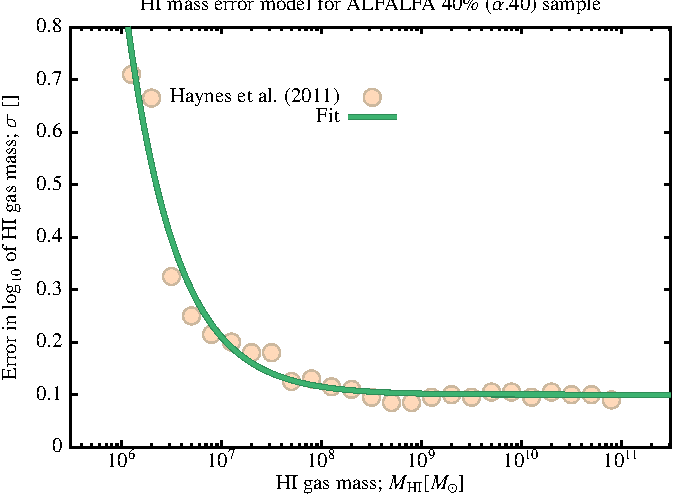
\includegraphics[width=85mm,trim=0mm 0mm 0mm 4mm,clip]{Plots/DataAnalysis/alfalfaHIMassErrorModel.pdf}
 \caption{The observational random error in galaxy HI mass as a function of HI mass for the ALFALFA survey. Points show the errors reported by \protect\cite{haynes_arecibo_2011}, while the line shows a simple functional form fit to these errors.}
 \end{center}
 \label{fig:ALFALFAErrorModel}
\end{figure}

Additionally, HI mass estimates can be affected by HI self-absorption for highly inclined galaxies. \cite[][see also \protect\citealt{zwaan_hipass_2005}]{zwaan_h_1997} estimate that this effect would lead to a mean underestimation of HI masses by a factor $1.1$ for a randomly oriented galaxy sample. Therefore, a value of $-0.0414$ for the systematic parameter {\normalfont \ttfamily [alfalfaHiMassFunctionZ0.00MassSystematic0]} is recommended.


\chapter{Input Data}

In some configurations, \glc\ requires additional input data to run. For example, if asked to process galaxy formation through a set of externally derived merger trees, then a file describing those trees must be given. In the remainder of this section we describe the structure of external datasets which can be inputs to \glc.

\section{Broadband Filters}\index{filters!broadband}

To compute luminosities through a given filter, \glc\ requires the response function, $R(\lambda)$, of that filter to be defined. \glc\ follows the convention of \cite{hogg_k_2002} in defining the filter response to be the fraction of incident photons received by the detector at a given wavelength, multiplied by the relative photon response (which will be 1 for a photon-counting detector such as a CCD, or proportional to the photon energy for a bolometer/calorimeter type detector. Filter response files are stored in {\normalfont \ttfamily data/filters/}. Their structure is shown below, with the {\normalfont \ttfamily SDSS\_g.xml} filter reponse file used as an example:
\begin{verbatim}
 <filter>
  <description>SDSS g vacuum (filter+CCD +0 air mass)</description>
  <name>SDSS g</name>
  <origin>Michael Blanton</origin>
  <response>
    <datum>   3630.000      0.0000000E+00</datum>
    <datum>   3680.000      2.2690000E-03</datum>
    <datum>   3730.000      5.4120002E-03</datum>
    <datum>   3780.000      9.8719997E-03</datum>
    <datum>   3830.000      2.9449999E-02</datum>
    .
    .
    . 
  </response>
  <effectiveWavelength>4727.02994472695</effectiveWavelength>
  <vegaOffset>0.107430167298754</vegaOffset>
</filter>
\end{verbatim}
The {\normalfont \ttfamily description} tag should provide a description of the filter, while the {\normalfont \ttfamily name} tag provides a shorter name. The {\normalfont \ttfamily origin} tag should describe from where/whom this filter originated. The {\normalfont \ttfamily response} element contains a list of {\normalfont \ttfamily datum} tags each giving a wavelength (in Angstroms) and response pair. The normalization of the response is arbitrary. The {\normalfont \ttfamily effectiveWavelength} tag gives the mean, response-weighted wavelength of the filter and is used, for example, in dust attenuation calculations. The {\normalfont \ttfamily vegaOffset} tag gives the value (in magnitudes) which must be added to an AB-system magnitude in this system to place it into the Vega system. Both {\normalfont \ttfamily effectiveWavelength} and {\normalfont \ttfamily vegaOffset} can be computed by running
\begin{verbatim}
 scripts/filters/vega_offset_effective_lambda.pl data/filters
\end{verbatim}
which will compute these values for any filter files that do not already contain them and append them to the files.

\section{Merger Trees}\label{sec:MergerTreeFiles}

While \glc\ can build merger trees using analytic methods it is often useful to be able to utilize merger trees from other sources (e.g. extracted from an N-body simulation). To facilitate this, \glc\ allows merger trees to be read from an HDF5 file\footnote{The following assumes that merger trees will be read from a file following \protect\glc's standard HDF5 format which is described in \S\protect\ref{sec:MergerTreeFileFormat}. Other formats can also be read by selecting the relevant importer via the {\normalfont \ttfamily [mergerTreeImporterMethod]} parameter.}. To do so, set the {\normalfont \ttfamily [mergerTreeConstructMethod]} input parameter to {\normalfont \ttfamily read} and specify the filename to read via their {\normalfont \ttfamily [mergerTreeReadFileName]} parameter.

The HDF5 file should follow the general purpose format described in \S\ref{sec:MergerTreeFileFormat}. An example of how to construct such a file can be found in the {\normalfont \ttfamily tests/nBodyMergerTrees} folder. In that folder, the {\normalfont \ttfamily getMillenniumTrees.pl} script will retrieve a sample of merger trees from the \href{http://www.g-vo.org/MyMillennium3/}{Millennium Simulation database} and use the {\normalfont \ttfamily Merger\_Tree\_File\_Maker.exe} code supplied with \glc\ to convert these into an HDF5 file suitable for reading into \glc. The {\normalfont \ttfamily getMillenniumTrees.pl} script requires you to have a username and password to access the Millennium Simulation database\footnote{If you do not have a username and password for the Millennium Simulation database you can request one from \href{mailto:contact@g-vo.org}{\normalfont \ttfamily contact@g-vo.org}.}. These can be entered manually or stored in a section of the {\normalfont \ttfamily galacticusConfig.xml} file (see \S\ref{sec:ConfigFile}) as follows:
\begin{verbatim}
  <millenniumDB>
    <host>
      <name>^myHost$</name>
      <user>myUserName</user>
      <passwordFrom>input</passwordFrom>
      <treePath>/path/to/trees</treePath>
    </host>
    <host>
      <name>default</name>
      <user>myUserName</user>
      <password>myPassword</password>
    </host>
  </millenniumDB>
\end{verbatim}
Here, each {\normalfont \ttfamily host} section describes rules for a given computer (with ``default'' being used if no specific match to the regular expression give in {\normalfont \ttfamily name} is found). The {\normalfont \ttfamily user} element gives the user name to use, while the {\normalfont \ttfamily passwordFrom} element specifies how the password should be obtained. Currently the only allowed mechanism is ``input'', in which case the password is read from standard input. Alternatively, you can include a {\normalfont \ttfamily password} element which contains the password itself. Of course, this is insecure\ldots

The optional {\normalfont \ttfamily treePath} element gives the location where merger trees from the Millennium Simulation can be stored. Some scripts will make use of this location so that Millennium Simulation merger trees can be shared between multiple scripts.

\subsection{Processing of Merger Tree Files}\label{sec:MergerTreeFileProcessing}

The ``read'' merger tree construction method (see \S\ref{sec:MergerTreeConstruction}) reads these files and processes them into a form suitable for \glc\ to evolve. Merger trees are inherently complex structures, particularly when the possibility of subhalos are considered. \glc\ is currently designed to work with single descendent merger trees, i.e. ones in which the tree structure is entirely defined by specifying which \gls{node} a given \gls{node} is physically associated with at a later time. Additionally, \glc\ expects the merger tree file to contain information on the host \gls{node}, i.e. the node within which a given node is physically located. In the following, these two properties are labelled {\normalfont \ttfamily descendentNode} and {\normalfont \ttfamily hostNode}. \glc\ assumes that nodes for which {\normalfont \ttfamily descendentNode}$=${\normalfont \ttfamily hostNode} are isolated halos (i.e. they are their own hosts) while other nodes are subhalos (i.e. they are hosted by some other node). An example of a simple tree structure is shown in Fig.~\ref{fig:MergerTreeSimple}. The particular structure would be represented by the following list of nodes and node properties (a $-1$ indicates that no descendent node exists):
\begin{center}
\begin{tabular}{rrr}
\hline
{\normalfont \ttfamily node} & {\normalfont \ttfamily descendentNode} & {\normalfont \ttfamily hostNode} \\
\hline
1 & -1 & 1 \\
2 &  1 & 2 \\
3 &  2 & 3 \\
4 &  1 & 4 \\
5 &  4 & 5 \\
6 & -1 & 1 \\
7 &  6 & 4 \\
8 &  7 & 8 \\
\hline
\end{tabular}
\end{center}

\begin{figure}
 \begin{center}
 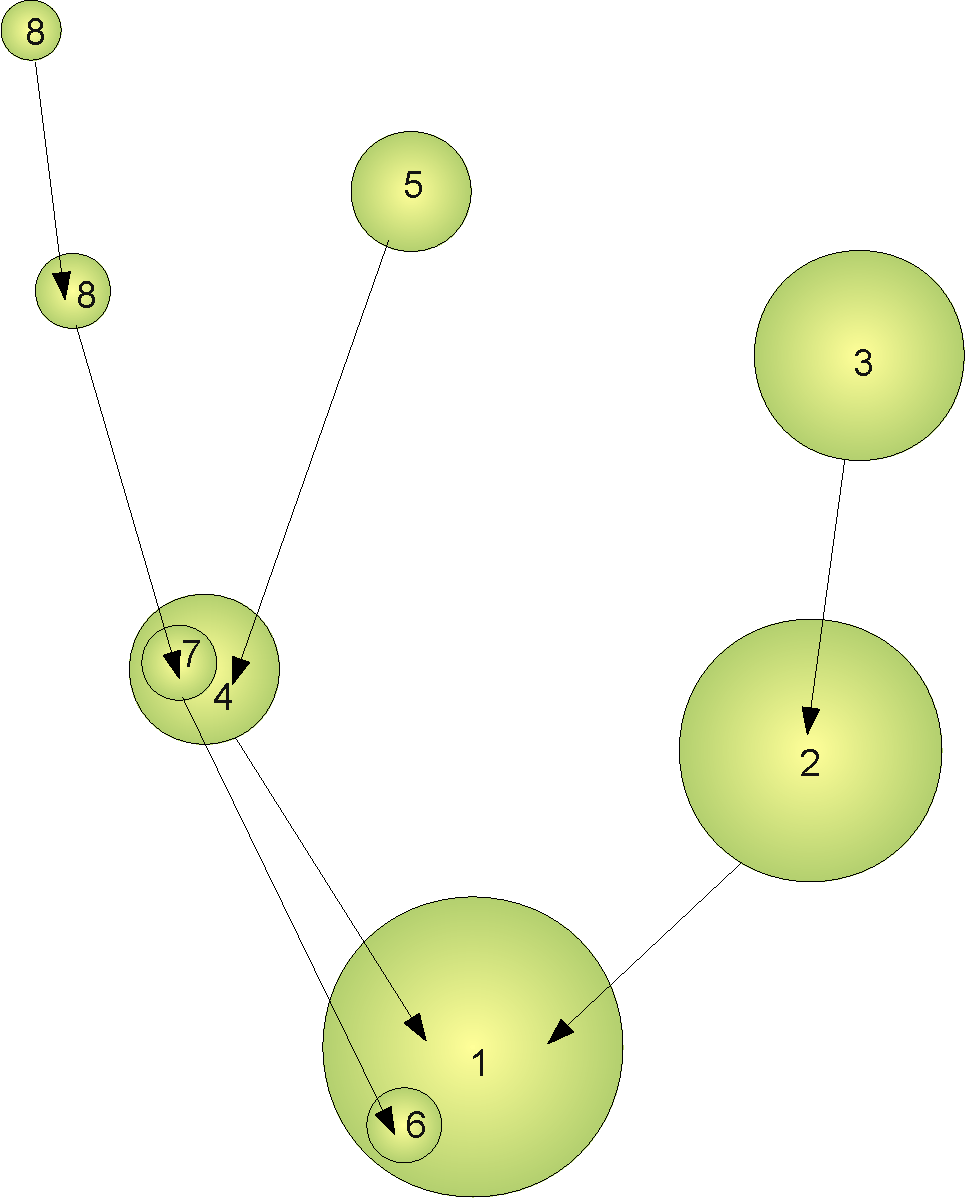
\includegraphics[width=160mm]{Diagrams/MergerTreeSimple.pdf}
 \end{center}
 \caption{An example of a simple merger tree structure. Colored circles represent nodes in the merger tree. Each node has a unique index indicated by the number inside each circle. Black arrows link each node to its descendent node (as specified by the {\normalfont \ttfamily descendentNode} property. Where a node is not its own host node it is placed inside its host node.}
 \label{fig:MergerTreeSimple}
\end{figure}

The following should be noted when constructing merger tree files:
\begin{itemize}
\item Note that \glc\ does not require that nodes be placed on a uniform grid of times/redshifts, nor that mass be conserved along a branch of the tree. After processing the tree in this way, \glc\ builds additional links which identify the child node of each halo and any sibling nodes. These are not required to specify the tree structure but are computationally convenient.
\item It is acceptable for a node to begin its existence as a subhalo (i.e. to have never had an isolated node progenitor). Such nodes will be created as satellites in the merger tree and, providing the selected node components (see \S\ref{sec:Components}) initialize their properties appropriately, will be evolved correctly.
\item It is acceptable for an isolated node to have progenitors, none of which are a primary progenitor. This can happen if all progenitors descend into subhalos in the isolated node. In such cases, \glc\ will create a clone of the isolated node at a very slightly earlier time to act as the primary progenitor. This is necessary to allow the tree to be processed correctly, but does not affect the evolution of the tree.
\item Normally, cases where a node's host node cannot be found in the \gls{forest} will cause \glc\ to exit with an error. Setting {\normalfont \ttfamily [mergerTreeReadMissingHostsAreFatal]}$=${\normalfont \ttfamily false} will instead circumvent this issue by making any such nodes self-hosting (i.e. they become isolated nodes rather than subhalos). Note that this behavior is not a physically correct way to treat such cases---it is intended only to allow trees to be processed in cases where the full \gls{forest} is not available.
\item It is acceptable for nodes to jump between branches in a tree, or even to jump between branches in different trees. In the latter case, all trees linked by jumping nodes (a so-called ``\gls{forest}'' of connected trees) must be stored as a single forest (with multiple root-nodes) in the merger tree file. \glc\ will process this \gls{forest} of trees simultaneously, allowing to nodes to move between their branches.
\item It is acceptable for a subhalo to later become an isolated halo (as can happen due to three-body interactions; see  \citealt{sales_cosmic_2007}). If {\normalfont \ttfamily [mergerTreeReadAllowSubhaloPromotions]}$=${\normalfont \ttfamily true} then such cases will be handled correctly (i.e. the subhalo will be promoted back to being an isolated halo). If {\normalfont \ttfamily [mergerTreeReadAllowSubhaloPromotions]}$=${\normalfont \ttfamily false} then subhalos are not permitted to become isolated halos. In this case, the following logic will be applied to remove all such cases from the tree:\\

\noindent\hspace{ 5mm} $\rightarrow$ \parbox[t]{150mm}{For any branch in a tree which at some point is a subhalo:}\\

\noindent\hspace{10mm} $\rightarrow$ \parbox[t]{145mm}{Beginning from the earliest node in the branch that is a subhalo, repeatedly step to the next descendent node;}\\

\noindent\hspace{10mm} $\rightarrow$ \parbox[t]{145mm}{If that descendent is \emph{not} a subhalo then:}\\

\noindent\hspace{15mm} $\rightarrow$ \parbox[t]{140mm}{If there is not currently any non-subhalo node which has the present node as its descendent then current node is only descendent of a subhalo. Therefore, try to make this node a subhalo, and propose the descendent of the host node of the previous node visited in the branch as the new host:}\\

\noindent\hspace{20mm} $\rightarrow$ \parbox[t]{135mm}{If the proposed host exists:}\\

\noindent\hspace{25mm} $\rightarrow$ \parbox[t]{130mm}{If the mass of the current node is less than that of the proposed host:}\\

\noindent\hspace{30mm} $\rightarrow$ \parbox[t]{125mm}{If the proposed hosts exists before the current node, repeatedly step to its descendents until one is found which exists at or after the time of the current node. This is the new proposed host.}\\

\noindent\hspace{30mm} $\rightarrow$ \parbox[t]{125mm}{If the proposed host is a subhalo, make it an isolated node.}\\

\noindent\hspace{30mm} $\rightarrow$ \parbox[t]{125mm}{The current node is made a subhalo within the proposed host.}\\

\noindent\hspace{25mm} $\rightarrow$ \parbox[t]{130mm}{Otherwise:}\\

\noindent\hspace{30mm} $\rightarrow$ \parbox[t]{125mm}{The current node remains an isolated node, while the proposed host is instead made a subhalo within the current node.}\\

\noindent\hspace{20mm} $\rightarrow$ \parbox[t]{135mm}{Otherwise:}\\

\noindent\hspace{25mm} $\rightarrow$ \parbox[t]{130mm}{The proposed host does not exists, which implies the end of a branch has been reached. Therefore, flag the current node as being a subhalo with a host identical to that of the node from which it descended.}\\
\end{itemize}

\subsubsection{Requirements for \glc\ Input Parameters}

The following requirements must be met for the input parameters to \glc\ when using merger trees read from file:
\begin{itemize}
 \item The cosmological parameters ($\Omega_\mathrm{M}$, $\Omega_\Lambda$, $\Omega_\mathrm{b}$, $H_0$, $\sigma_8$), if defined in the file, must be set identically in the \glc\ input file unless you set {\normalfont \ttfamily [mergerTreeReadMismatchIsFatal]}$=${\normalfont \ttfamily false} in which case you'll just be warned about any mismatch;
 \item \glc\ assumes by default that all merger trees exist at the final output time---if this is not the case set {\normalfont \ttfamily [allTreesExistAtFinalTime]}$=${\normalfont \ttfamily false}.
\end{itemize}

\subsection{Setting of Halo Properties}

\subsubsection{Dark Matter Scale Radii}\index{dark matter halo!concentration}\index{dark matter halo!scale radius}

If {\normalfont \ttfamily [mergerTreeReadPresetScaleRadii]}$=${\normalfont \ttfamily true} and the {\normalfont \ttfamily halfMassRadius} dataset is available within the {\normalfont \ttfamily haloTrees} group (see \S\ref{sec:ForestHalosGroup}) then the half-mass radii of nodes will be used to compute the corresponding scale length of the dark matter halo profile\footnote{The scale radius is found by seeking a value which gives the correct half mass radius. It is therefore important that the definition of halo mass (specifically the virial overdensity) in \protect\glc\ be the same as was used in computing the input half mass radii.}. This requires a dark matter profile scale component which supports setting of the scale length (see \S\ref{sec:DarkMatterProfileComponent}).

\subsubsection{Satellite Merger Times}\index{merger times}\index{satellite!merger times}

If {\normalfont \ttfamily [mergerTreeReadPresetMergerTimes]}$=${\normalfont \ttfamily true} then merger times for satellites will be computed directly from the merger tree data read from file. When a subhalo has an isolated halo as a descendent it is assumed to undergo a merger with that isolated halo at that time. Note that this requires a satellite orbit component method which supports setting of merger times (e.g. {\normalfont \ttfamily [treeNodeMethodSatelliteOrbit]}$=${\normalfont \ttfamily preset}).

\subsubsection{Dark Matter Halo Spins}\index{dark matter halo!spin}

If {\normalfont \ttfamily [mergerTreeReadPresetSpins]}$=${\normalfont \ttfamily true} and the {\normalfont \ttfamily angularMomentum} dataset is available within the {\normalfont \ttfamily haloTrees} group (see \S\ref{sec:ForestHalosGroup}) then the spin parameters of nodes will be computed and set. This requires a dark matter halo spin component which supports setting of the spin (see \S\ref{sec:DarkMatterHaloSpinComponent}).


\chapter{Constraining {\sc Galacticus}}

\section{Model Accuracy}\label{sec:ModelAccuracy}

The model accuracy script processes the model described by a standard \glc\ constraints configuration file to assess how accurate the model is. Specifically, it determines the relative contribution to the covariance of each constraint arising from the finite number of merger trees run in the model and the intrinsic covariance of the observations. An accurate model should make a negligible contribution to the covariance.

To run the model accuracy script use
\begin{verbatim}
 constraints/testModelAccuracy.pl <configFile>
\end{verbatim}
where {\tt configFile} is the name of the configuration file. The script will run the model multiple times, reducing the number of trees per decade by a factor of two each time (this is done 8 times, such that the smallest model run has a factor 128 times fewer trees than the original model). Furthermore, this sequence of models is run for three different choices for sampling halo masses: {\tt powerLaw}, {\tt haloMassFunction}, and {\tt stellarMassFunction} (see \S\ref{sec:MassSamplingDensityFunction}).

For each constraint in the specified constraint compilation and accuracy measure is constructed which is the root mean squared ratio of the error arising from the finite number of trees and the intrinsic error of the constraint data. 

Accuracy analysis files are written to:
\begin{verbatim}
 <workDirectory>/accuracy
\end{verbatim}
For each constraint in the compilation a plot showing accuracy measure as a function of CPU time is written to
\begin{verbatim}
 <constraintLabel>_mergerTreeBuildTreesPerDecade.pdf
\end{verbatim}
Each point in the plot is labelled with the number of merger trees per decade. An accurate model should have accuracy measure significantly below unity. This plot is also useful to see which sampling method achieves that accuracy in the least amount of CPU time.

Additionally, a report is written to:
\begin{verbatim}
 <constraintLabel>Report.txt
\end{verbatim}
This file lists, for each sampling method, the accuracy measure achieved and the CPU time taken for the largest model run.

\section{Model Convergence}\label{sec:ModelConvergence}

The model convergence script processes the model described by a standard \glc\ constraints configuration file to assess how well converged the model is with respect to several of \glc's numerical parameters. Specifically, it determines the a covariance measure for each constraint in the specified compilation file.

To run the model convergence script use
\begin{verbatim}
 constraints/testConvergnce.pl <configFile>
\end{verbatim}
where {\tt configFile} is the name of the configuration file. The script will run the model multiple times, adjusting the value of a numerical parameter each time.

For each constraint in the specified constraint compilation a convergence measure, $C$, is constructed which
\begin{equation}
 C = \sum_i {(y_i - y_{{\rm ideal}, i})^2 \over \sqrt{2} \sigma_{{\rm ideal}, i}^2}
\end{equation}
where $y_i$ is the result of the constraint, $\sigma_i$ is the error on the result, and subscript ``ideal'' refers to the model with the most ideal value (i.e. that in the original, unmodified model) of the numerical parameter being tested (which might be the lowest value for a mass resolution, or the highest value for the maximum tree mass simulated for example). To be converged, the convergence measure should remain consistent with unity within a significant distance\footnote{``Significant distance'' here requires some judgement. Typically we would like for the model results to not change significantly as the value of a numerical parameter is adjusted by at least a factor of 2 away from the ideal value.} away from the ideal value.

Convergence analysis files are written to:
\begin{verbatim}
 <workDirectory>/convergence
\end{verbatim}
For each combination of constraint in the compilation and numerical parameter a plot showing the convergence measure as a function of the numerical parameter is created in:
\begin{verbatim}
 <constraintLabel>_<numericalParameter>.pdf
\end{verbatim}
Each point in the plot has an error bar since, due to the limited number of merger trees run, the convergence measure is not known with perfect precision. A horizontal line shows the desired convergence measure of unity.

Additionally, a report is written to:
\begin{verbatim}
 <constraintLabel>Report.txt
\end{verbatim}
This file lists, for each numerical parameter, the convergence measure and its error achieved by the ideal model. Additionally a normalized measure (the measure divided by its error) is listed. This normalized measure can be approximately interpretted as the number of $\sigma$ deviation from convergence.

\section{Model Discrepancy}\label{sec:ModelDiscrepancy}

Model discrepancy scripts process the model described by a standard \glc\ constraints configuration file to produce an output HDF5 file which describes a particular contribution to the model discrepancy. The format of these files is
\begin{verbatim}
HDF5 "discrepancy.hdf5" {
GROUP "/" {
   DATASET "additive" {
   }
   DATASET "multiplicative" {
   }
   DATASET "covariance" {
   }
}
\end{verbatim}
Each of the three datasets is optional (i.e. not all need be provided for each discrepancy). The {\tt additive} dataset gives an additive offset which will be applied to the relevant model results. The {\tt multiplicative} dataset similarly gives a multiplicative offset which will be applied to the relevant model results. Finally, the {\tt covariance} dataset gives the contribution from this discrepancy to the covariance matrix used in evaluating the model likelihood.

Discrepancy files are written to
\begin{verbatim}
 <workDirectory>/modelDiscrepancy/<discrepancyLabel>/discrepancy<constraintLabel>.hdf5
\end{verbatim}

Constraint scripts (see \S\ref{sec:ConstraintScripts}) accept a command line option {\tt --modelDiscrepancies} which specifies the path to the {\tt modelDiscrepancy} directory (i.e. {\tt <workDirectory>/modelDiscrepancy}) and will search for any relevant model discrepancy files and apply them in their calculations.

\subsection{Monte Carlo Merger Trees}

\glc\ typically uses Monte Carlo-generated merger trees when being constrained to fit data. These have the advantage that they can be generated for any cosmological parameters (necessary if the cosmological parameters are to be varied as part of the constraining process) and they can be generated uniquely for each model evaluation which avoids any bias introduced by using a fixed set of halos.

However, these Monte Carlo-generated trees may not precisely capture the properties of merger trees derived from a fully non-linear calculation of gravitational collapse (e.g. as performed by an N-body simulation). Therefore it is important to assess the model discrepancy arising from this limitation.

Model discrepancy files can be generated using:
\begin{verbatim}
 constraints/modelDiscrepancy/monteCarloTrees.pl config.xml
\end{verbatim}
where {\tt config.xml} is a standard \glc\ constraint configuration file. The script will run two sets of models, one using N-body merger trees derived from the \gls{millenniumSimulation}, and a second using Monte Carlo-generated merger trees. The number of subvolumes of the \gls{millenniumSimulation} to use is specified by the {\tt subVolumeCount} option to this script (a default of $32$ subvolumes is used if no number is specified). The subvolume data will be downloaded from the \gls{millenniumSimulation} database if necessary.

To make a fair comparison, \gls{millenniumSimulation} merger trees have their branches pruned below a mass corresponding to $20$ particles, and the Monte Carlo merger trees are built with the equivalent mass resolution. Additionally, the Monte Carlo merger trees are regridded onto a set of timesteps matched to the \gls{millenniumSimulation}.

A multiplicative model discrepancy is computed for each constraint included in the compilation (as specified in the configuration file) equal to the ratio of the N-body result to the Monte Carlo result. Additionally, the subvolumes of the \gls{millenniumSimulation} are used to estimate the covariance in the N-body result due to the finite volume of the simulation. The result is computed for each subvolume separately and the covariance of the result between subvolumes computed. This is repeated using pairs of subvolumes, quads of subvolumes, etc. If $2^n$ subvolumes were used, then the covariance measured from the result combining $2^{n-3}$ subvolumes is used to extrapolate the covariance for all $512$ subvolumes assuming that the covariance scales in inverse proportion to the number of subvolume used. Finally, the contribution of the Monte Carlo trees model to the covariance is assumed to be a diagonal matrix with elements equal to the square of the reported errors on the result of the model.

\subsection{Fixed Virial Orbits}

The orbital parameters of subhalos at the point of virial orbit crossing are usually drawn from an appropriate cosmological distribution. If instead fixed virial orbital parameters are used instead then term should be included in the model discrepancy accounting for this approximation. 

Model discrepancy files can be generated using:
\begin{verbatim}
 constraints/modelDiscrepancy/fixedVirialOrbits.pl config.xml
\end{verbatim}
where {\tt config.xml} is a standard \glc\ constraint configuration file. The script will run two models, one using fixed virial orbital parameters, and a second using variable orbital parameters using the {\tt Benson2005} method (see \S\ref{sec:VirialOrbitsBenson2005}). A multiplicative model discrepancy is computed for each constraint included in the compilation (as specified in the configuration file) equal to the ratio of the variable orbits result to the fixed orbits result. Additionally, a model discrepancy covariance is computed. This is assumed to be a diagonal matrix with elements equal to the square of the reported errors on the results of the fixed and variable orbital parameters models.

\subsection{Jiang et al. (2008) Merger Time Scatter}

The \cite{jiang_fitting_2008} algorithm for the merging times of dark matter subhalos includes drawing times from a log-normal distribution of width $\sigma=0.4$ with median equal to their fitting function (see \S\ref{sec:DynamicalFrictionJiang2008}). If instead zero scatter is used then a term should be included in the model discrepancy accounting for this approximation. 

Model discrepancy files can be generated using:
\begin{verbatim}
 constraints/modelDiscrepancy/jiang2008MergingTimeScatter.pl config.xml
\end{verbatim}
where {\tt config.xml} is a standard \glc\ constraint configuration file. The script will run two models, one using the default scatter specified by the configuration file, and a second using $\sigma=0.4$. A multiplicative model discrepancy is computed for each constraint included in the compilation (as specified in the configuration file) equal to the ratio of the $\sigma=0.4$ and default scatter results. Additionally, a model discrepancy covariance is computed. This is assumed to be a diagonal matrix with elements equal to the sum of the square of the reported errors on the result of the default scatter and $\sigma=0.4$ models.

\section{Optimal Halo Mass Function Sampling}

Suppose we want to fit parameters of the \glc\ model to some dataset. The basic approach is to generate large numbers of model realizations for different parameter values and see which ones best match the data. \glc\ models involve simulating individual merger trees and then adding together their galaxies to produce some overall function. The question we want to answer is, given some finite amount of computing time, what is the optimal distribution of halo masses to run when comparing to a given dataset. For example, is it better to run a volume limited sample (as one would get from an N-body simulation) or is it better to use, say, equal numbers of halos per logarithmic interval of halo mass? The following section describes how to solve this optimization problem in the specific case of fitting to the stellar mass function.

\subsection{Li \& White (2009) Stellar Mass Function}\label{sec:OptimalSamplingStellarMassFunction}

First, some definitions:
\begin{description}
 \item [$n(M) \d \ln M$] is the dark matter halo mass function, i.e. the number of halos in the range $M$ to $M+M\d\ln  M$ per unit volume;
 \item [$\gamma(M) \d \ln M$] is the number of trees that we will simulate in the range $M$ to $M+M\d \ln M$;
 \item [$\alpha(M_\star)$] is the error on the observed stellar mass function at mass $M_\star$;
 \item [$P(N|M_\star,M;\delta \ln M_\star)$] is the conditional stellar mass distribution function of galaxies of stellar mass $M_\star$ in a bin of width $\delta \ln M_\star$ per halo of mass $M$;
 \item [$t(M)$] is the CPU time it takes to simulate a tree of mass $M$.
\end{description}
To clarify, $P(N|M_\star,M;\delta \ln M_\star;\delta \ln M_\star)$ is the probability\footnote{To put it another way, $P(N|M_\star,M;\delta \ln M_\star)$ is closely related to the commonly used Halo Occupation Distribution.} to find $N$ galaxies of mass between $M_\star$ in a bin of width $\delta \ln M_\star$ in a halo of mass $M$. The usual conditional stellar mass function is simply the first moment of this distribution:
\begin{equation}
 \phi(M_\star;M) \delta \ln M_\star = \sum_{N=0}^\infty N P(N|M_\star,M;\delta \ln M_\star)
 \label{eq:cSMFdefinition}
\end{equation}
The model estimate of the stellar mass function $\Phi(M_\star)$ (defined per unit $\ln M_\star$) is
\begin{equation}
 \Phi(M_\star) = \int_0^\infty \phi(M_\star;M) {n(M) \over \gamma(M)} \gamma(M) \d \ln M,
\end{equation}
where the $n(M)/\gamma(M)$ term is the weight assigned to each tree realization---and therefore the weight assigned to each model galaxy when summing over a model realization to construct the stellar mass function. 

When computing a model likelihood, we must employ some statistic which defines how likely the model is given the data. Typically, for stellar mass functions we have an estimate of the variance in the data, $\alpha^2(M_\star)$, as a function of stellar mass (full covariance matrices are typically not provided but, ideally would be, and can be easily incorporated into this method). In that case, we can define a likelihood
\begin{equation}
 \ln \mathcal{L} = - {1 \over 2} \sum_i {[\phi_{{\rm obs},i} - \phi_i]^2 \over \alpha_i^2 + \sigma_i^2}
\end{equation}
where the sum is taken over all data points, $i$, and $\sigma_i^2$ is the variance in the model estimate and is given by
\begin{equation}
 \sigma^2(M_\star) = \langle [\phi(M_\star) - \bar{\phi}(M_\star)]^2 \rangle,
\end{equation}
where $\phi(M_\star)$ is the realization from a single model and $\bar{\phi}(M_\star)$ is the model expectation from an infinite number of merger tree realizations and the average is taken over all possible model realizations. Since the contributions from each merger tree are independent, 
\begin{equation}
 \sigma^2(M_\star) = \sum_i \zeta_i^2(M_\star;M)
\end{equation}
where $\zeta_i^2(M_\star;M)$ is the variance in the contribution to the stellar mass function from tree $i$. This in turn is given by
\begin{equation}
 \zeta^2(M_\star;M) = \psi^2(M_\star;M) \left[{n(M) \over \gamma(M)}\right]^2,
\end{equation}
where $\psi^2(M_\star;M)$ is the variance in the conditional stellar mass function. In the continuum limit this becomes
\begin{equation}
 \sigma^2(M_\star) = \int_0^\infty \psi^2(M_\star;M) \left[{n(M) \over \gamma(M)}\right]^2 \gamma(M) \d \ln M.
\end{equation}

Model variance artificially increases the likelihood of a given model. We would therefore like to minimize the increase in the likelihood due to the model variance:
\begin{equation}
\Delta 2 \ln \mathcal{L} = \sum_i {[\phi_{{\rm obs},i} - \phi_i]^2 \over \alpha_i^2} - {[\phi_{{\rm obs},i} - \phi_i]^2 \over \alpha_i^2 + \sigma_i^2} 
\end{equation}
Of course, we don't know the model prediction, $\phi_i$, in advance\footnote{Below, we will adopt a simple empirical model for $\phi(M_\star)$. However, it should not be used here since we will in actuality be computing the likelihood from the model itself.}. However, if we assume that a model exists which is a good fit to the data then we would expect that $[\phi_{{\rm obs},i} - \phi_i]^2 \approx \alpha_i^2$ on average. In that case, the increase in likelihood due to the model is minimized by minimizing the function\footnote{This can be seen intuitively: we are simply requring that the variance in the model prediction is small compared the the variance in the data.}
\begin{equation}
 F[\gamma(M)] = \sum_i {\alpha_i^2 \over \alpha_i^2 + \sigma_i^2}.
\end{equation}
If the bins all have the same $\delta \ln M_\star$ we can turn the sum into an integral
\begin{equation}
 F[\gamma(M)] = \int_0^\infty {\alpha(M_\star)^2 \over \alpha(M_\star)^2 + \sigma(M_\star)^2} \d \ln M_\star.
\end{equation}
Obviously, the answer is to make $\gamma(M)=\infty$, in which case $ F[\gamma(M)]=0$. However, we have finite computing resources. The total time to run our calculation is
\begin{equation}
 \tau = \int_0^\infty t(M) \gamma(M) \d \ln M.
\end{equation}
We therefore want to minimize $F[\gamma(M)]$ while keeping $\tau$ equal to some finite value. We can do this using a Lagrange multiplier and minimizing the function
\begin{equation}
  F[\gamma(M)] = \int_0^\infty {\alpha(M_\star)^2 \over \alpha(M_\star)^2 + \sigma(M_\star)^2} \d \ln M_\star + \int_0^\infty \lambda \gamma(M) t(M) \d \ln M.
\end{equation}
Finding the functional derivative and setting it equal to zero gives:
\begin{equation}
 \gamma(M) = \sqrt{{\xi(M) \over \lambda t(M)}},
\end{equation}
in the limit where\footnote{This is the limit in which we would like our results to be.} $\sigma(M_\star) \ll \alpha(M_\star)$, and where
\begin{equation}
 \xi(M) = n^2(M) \int_{-\infty}^\infty {\psi^2(M_\star;M) \over \alpha^2(M_\star)} \d \ln M_\star.
\end{equation}
The values of $\lambda$ and $\delta \ln M_\star$, and the normalization of $t(M)$ are unimportant here since we merely want to find the optimal shape of the $\gamma(M)$ function---we can then scale it up or down to use the available time.

Figure~\ref{fig:optimalSamplingStellarMassFunction} shows the function $\gamma(M)$ obtained by adopting a model conditional stellar mass function which is a sum of central and satellite terms. Specifically, we use the model of \cite{leauthaud_new_2011} which is constrained to match observations from the COSMOS survey. In their model\footnote{This integral form of the conditional stellar mass function is convenient here since it allows for easy calcualtion of the number of galaxies expected in the finite-width bins of the observed stellar mass function.}:
\begin{equation}
 \langle N_{\rm c}(M_\star|M)\rangle \equiv \int_{M_\star}^\infty \phi_{\rm c}(M_\star^\prime) \d \ln M_\star^\prime = {1 \over 2} \left[ 1 - \hbox{erf}\left( {\log_{10}M_\star - \log_{10} f_{\rm SHMR}(M) \over \sqrt{2}\sigma_{\log M_\star}} \right) \right].
\end{equation}
Here, the function $f_{\rm SHMR}(M)$ is the solution of
\begin{equation}
 \log_{10}M = \log_{10}M_1 + \beta \log_{10}\left({M_\star \over M_{\star,0}}\right) + {(M_\star/M_{\star,0})^\delta \over 1 + (M_\star/M_{\star,0})^{-\gamma}} - {1/2}.
\end{equation}
For satellites,
\begin{equation}
 \langle N_{\rm s}(M_\star|M)\rangle \equiv \int_{M_\star}^\infty \phi_{\rm s}(M_\star^\prime) \d \ln M_\star^\prime =  \langle N_{\rm c}(M_\star|M)\rangle \left({f^{-1}_{\rm SHMR}(M_\star) \over M_{\rm sat}}\right)^{\alpha_{\rm sat}} \exp\left(- {M_{\rm cut} \over f^{-1}_{\rm SHMR}(M_\star)} \right),
\end{equation}
where
\begin{equation}
 {M_{\rm sat} \over 10^{12} M_\odot} = B_{\rm sat} \left({f^{-1}_{\rm SHMR}(M_\star) \over 10^{12} M_\odot}\right)^{\beta_{\rm sat}},
\end{equation}
and
\begin{equation}
 {M_{\rm cut} \over 10^{12} M_\odot} = B_{\rm cut} \left({f^{-1}_{\rm SHMR}(M_\star) \over 10^{12} M_\odot}\right)^{\beta_{\rm cut}}.
\end{equation}

We use the best fit parameters from the {\tt SIG\_MOD1} method of \cite{leauthaud_new_2011} for their $z_1$ sample, but apply a shift of $-0.2$ dex in masses to bring the fit into line with the $z=0.07$ mass function of \cite{li_distribution_2009}. The resulting parameter values are shown in Table~\ref{tb:z0SMFFitParameters}.

\begin{table}
\begin{center}
\caption{Parameters of the conditional stellar mass function fit.}
\label{tb:z0SMFFitParameters}
\begin{tabular}{lr@{.}lr@{.}l}
\hline
{\bf Parameter} & \multicolumn{2}{c}{\bf Value} \\
\hline
$\alpha_{\rm sat}$& 1&0 \\
$\log_{10} M_1$& 12&120 \\
$\log_{10} M_{\star,0}$& 10&516 \\
$\beta$& 0&430 \\
$\delta$& 0&5666 \\
$\gamma$& 1&53 \\
$\sigma_{\log M_\star}$& 0&206 \\
$B_{\rm cut}$& 0&744 \\
$B_{\rm sat}$& 8&00 \\
$\beta_{\rm cut}$& $-$0&13 \\
$\beta_{\rm sat}$& 0&859 \\
\hline
\end{tabular}
\end{center}
\end{table}

We assume that $P_{\rm s}(N|M_\star,M;\delta \ln M_\star)$ is a Poisson distribution while $P_{\rm c}(N|M_\star,M;\delta \ln M_\star)$ has a Bernoulli distribution, with each distribution's free parameter fixed by the constraint of eqn.~(\ref{eq:cSMFdefinition}), and the assumed forms for $\phi_{\rm c}$ and $\phi_{\rm s}$.

The errors in the \cite{li_distribution_2009} observed stellar mass function are well fit by (see Fig.~\ref{fig:stellarMassFunctionErrors}):
\begin{equation}
 \alpha(M_\star) = 10^{-3} \left({M_\star\over 4.5\times 10^{10}M_\odot}\right)^{-0.3} \exp\left(-{M_\star\over 4.5\times 10^{10}M_\odot}\right) + 10^{-7},
 \label{eq:stellarMassFunctionErrorsFit}
\end{equation}
and the tree processing time in \glc\ can be described by:
\begin{equation}
 \log_{10} t(M) = \sum_{i=0}^2 C_i [ \log_{10} M ]^i
\end{equation}
with $C_0=-0.73$, $C_1=-0.20$ and $C_2=0.035$.

The resulting optimal sampling density curve is shown in Fig.~\ref{fig:optimalSamplingStellarMassFunction} and is compared to weighting by the halo mass function (i.e. the result of sampling halos at random from a representative volume). Optimal sampling gives less weight to low mass halos (since a sufficient accuracy can be obtained without the need to run many tens of thousands of such halos) and to high mass halos which are computationally expensive. 

\begin{figure}
 \begin{center}
 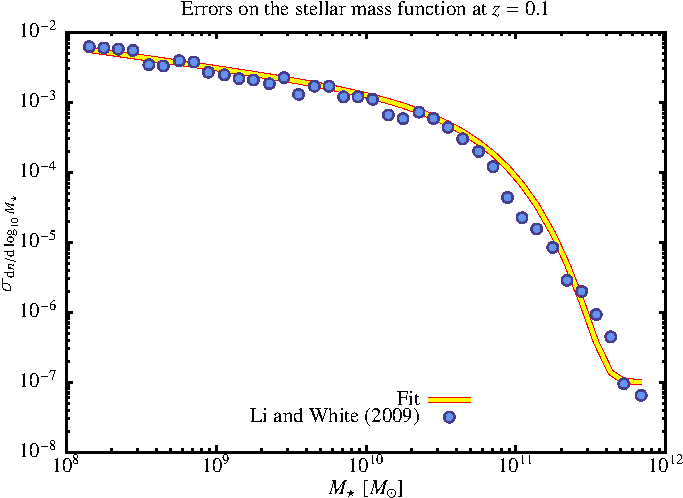
\includegraphics[width=160mm]{../plots/stellarMassFunctionErrors_z01.pdf}
 \end{center}
 \caption{Errors on the \protect\cite{li_distribution_2009} stellar mass funtion (points) and the fitting function (line) given by eqn.~(\protect\ref{eq:stellarMassFunctionErrorsFit}).}
 \label{fig:stellarMassFunctionErrors}
\end{figure}

\begin{figure}
 \begin{center}
 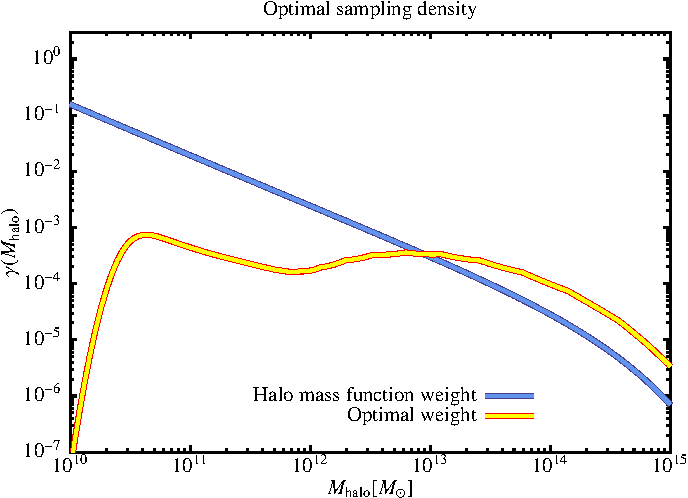
\includegraphics[width=160mm]{../plots/optimalSamplingStellarMassFunction.pdf}
 \end{center}
 \caption{Optimal weighting (yellow line) compared with weighting by the dark matter halo mass function (i.e. sampling halos at random from a representative volume; blue line). Sampling densities have been normalized to unit compute time.}
 \label{fig:optimalSamplingStellarMassFunction}
\end{figure}

\subsection{Refining by Other Merger Tree Statistics}

Since building merger trees is relatively fast, while solving the baryonic physics is slow it may be advantageous to  non-uniformly sample the distribution of merger trees at fixed merger tree mass, $M$. For example, we could assign some measure of formation history to each merger tree, such as the time since the last major merger, $\tau$. The halo mass function then becomes $n(M,\tau)$ (which can be computed by simulating large numbers of trees), and the tree sampling function becomes $\gamma(M,\tau)$. We'd then need to know the stellar mass function conditioned on both $M$ and $\tau$, $\phi_\star(M_\star|M,\tau)$. Given these, the above approach could be easily generalized to determine an optimal $\gamma(M,\tau)$. Then, after generating a merger tree, we'd first compute $\tau$. If a sufficient number of trees in that $\tau$ interval had already been computed, then we'd simply drop that tree and compute another one. The speed up here would depend on how fast building trees is relative to solving baryonic physics and what fraction of trees you discard. In principle, the trees could be generated, sampled and stored in advance so that we'd already have an optimally distributed set of trees in $M$ and $\tau$ that could be used for each model run.

\section{Constraints}\label{sec:ConstraintScripts}

Any constraint which can be applied to \glc\ is defined by two files, a configuration file and a likelihood script, which must be placed in {\tt constraints/constraints} and {\tt constraints/scripts} respectively. 

\subsection{Configuration File}\label{sec:ConstraintConfigFiles}

The configuration file should have the form:
\begin{verbatim}
<!-- Defines a constraint to match some data. -->                                          
<constraint>                                                                                                         
  <name>Long-form name of this constraint</name>                                                                      
  <label>shortLabelForThisConstraint</label>                                                                        
  <outputRedshift>0.07</outputRedshift>                                                                              
  <outputRedshift>1.00</outputRedshift>                                                                              
  <haloMassResolution>5.0e9</haloMassResolution>                                                                     
  <haloMassMinimum>2.0e10</haloMassMinimum>                                                                          
  <haloMassMaximum>2.0e14</haloMassMaximum>                                                                          
  <analysis>constraints/scripts/myAnalysisScript.pl</analysis>                                         
  <luminosity>
    <filter>UKIRT_K</filter>
    <redshift>0.0</redshift>
    <frame>rest</frame>
  </luminosity>
  <luminosity>
    <filter>UKIRT_K</filter>
    <redshift>1.0</redshift>
    <frame>observed</frame>
  </luminosity>
  <optionOn>outputMainBranchStatus</optionOn>
  <optionOn>outputDensityContrastData</optionOn>
  <parameter>
   <name>outputDensityContrastValues</name>
   <value>200.0</value>
   <accumulation>unique</accumulation>
  </parameter>
</constraint>                                                                                                        
\end{verbatim}
The {\tt name} and {\tt label} are used to describe the constraint ({\tt label} is used as a suffix in file names so should not contain spaces or other characters which might cause problems in file names). 

The remaining elements describe the requirements for this constraint. {\tt haloMassResolution} specifies the maximum resolution in mergers trees that still allows this constraint to be computed accurately. Similarly, {\tt haloMassMinimum} and {\tt haloMassMaximum} specify the required range of halo masses to simulate to allow this constraint to be computed accurately.

One or more {\tt outputRedshift} elements may be present, each specifying a redshift at which output is required for this constraint. Similarly, one or more {\tt luminosity} elements may be present, each of which specifies a luminosity which must be computed for this constraint. Each {\tt luminosity} must contain a specification of {\tt filter}, {\tt redshift}, and {\tt frame} to define which luminosity is to be computed.

One or more {\tt optionOn} elements may be present. Each element must specify the name of a \glc\ input parameter. That parameter will be set to {\tt true} in the \glc\ input parameter file.

Finally, arbitrary other parameter may be set using the standard {\tt parameter} element which should give the {\tt name} and {\tt value} for the parameter. Optionally, an {\tt accumulation} element may also be specified for each {\tt parameter}. This controls how values of the parameter are to be accumulated if set by more than one constraint. An accumulation of {\tt overwrite} will simply overwrite any previously set values. An accumulation of {\tt combine} will concatenate all values set by different constraints. Finally, an accumulation of {\tt unique} will concatenate all values set by different constraints and then filter out any duplicates.

When multiple constraints are used, their requirements are automatically combined.

\subsection{Likelihood Script}

The likelihood script for a constraint is required to perform several tasks, controlled by command line options. The script should accept the following command line syntax:
\begin{verbatim}
 myScript.pl <galacticusFile> [options...]
\end{verbatim}
where {\tt galacticusFile} is the file name of the \glc\ model for which the likelihood calculation should be performed. The following options must be supported by the script:
\begin{description}
 \item [{\tt --plotFile <fileName>}] If this option is present, the script should generate a plot showing the constraint and the model result and write it to {\tt fileName}.
 \item [{\tt --outputFile <fileName>}] If this option is present, the script should compute the log-likelihood of the model given the constraint and write it to {\tt fileName} using the format
\begin{verbatim}
 <constraint>
  <logLikelihood>-123</logLikelihood>
 </constraint>
\end{verbatim}
 \item [{\tt --accuracyFile <fileName>}] If this option is present, the script should write an XML file giving details of the accuracy of the model results relative to the observational errors using the format
\begin{verbatim}
 <accuracy>
  <x>...</x>
  .
  .
  .
  <x>...</x>
  <yModel>...</yModel>
  .
  .
  .
  <yModel>...</yModel>
  <yData>...</yData>
  .
  .
  .
  <yData>...</yData>
  <errorModel>...</errorModel>
  .
  .
  .
  <errorModel>...</errorModel>
  <errorData>...</errorData>
  .
  .
  .
  <errorData>...</errorData>
 </accuracy>
\end{verbatim}
In this file the {\tt yModel} and {\tt yData} elements should give the values of the model result and the comparable data respectively, while {\tt errorModel} and {\tt errorData} should give an estimate of the errors on these quantities. In the case of the model error this should include only the contribution arising from the finite number of merger trees simulated. This file will be used to judge whether the model is running sufficient merger trees such that the likelihood is not dominated by these errors. The {\tt x} elements are optional but can be used to give the parameter values associated with each model result.
 \item [{\tt --resultFile <fileName>}] If this option is present, the script should write an XML file giving details of the result of the model using the format
\begin{verbatim}
 <accuracy>
  <x>...</x>
  .
  .
  .
  <x>...</x>
  <y>...</y>
  .
  .
  .
  <y>...</y>
  <error>...</error>
  .
  .
  .
  <error>...</error>
 </accuracy>
\end{verbatim}
In this file the {\tt y} elements should give the values of the model result, while the {\tt error} elements should give an estimate of the errors on these results. The error should include only the contribution arising from the finite number of merger trees simulated. This file will be used to judge whether the model result is converged with respect to various numerical parameters in \glc. The {\tt x} elements are optional but can be used to give the parameter values associated with each model result.
 \item [{\tt --modelDiscrepancies <path>}] If this option is present, the script should scan {\tt path}. For each directory found in {\tt path} the script should check for the existance of a file named {\tt discrepancy<label>.hdf5} where {\tt label} is the label given for this constraint in its configuration file (see \S\ref{sec:ConstraintConfigFiles}). If present, the model discrepancy given in that file should be applied to the likelihood calculation. See \S\ref{sec:ModelDiscrepancy} for a description of the structure of the discrepancy files.
\end{description}

\subsection{Available Constraints}

\subsubsection{Li \& White (2009) SDSS Stellar Mass Function}

This constraint utilizes the stellar mass function for $z\approx 0.07$ galaxies measured by \cite{li_distribution_2009} from the \gls{sdss}. The mass function reported by \cite{li_distribution_2009} is converted to the appropriate Hubble constant for the given \glc\ model (assuming that masses scale as $H_0^{-2}$ and volumes as $H_0^3$)---no adjustment is made for cosmological parameters given the low redshift of the sample.

Given a \glc\ model, total stellar masses of model galaxies are adjusted using:
\begin{equation}
 M_\star \rightarrow {\bf G} {\bf S} M_\star 
\end{equation}
where the ${\bf S}$ operator is a multiplicative factor accounting for systematic errors in stellar mass determination and is equal to \citep{behroozi_comprehensive_2010}
\begin{equation}
 \log_{\rm 10} S = \mu + \kappa \log_{\rm 10} \left({M_\star \over 10^{11.3}M_\odot}\right)
\end{equation}
where $\mu=${\tt [sdssStellarMassFunctionZ0.07StellarMassSystematicMu]}, $\kappa=${\tt [sdssStellarMassFunctionZ0.07StellarMassSystematiKappa]}, and the {\bf G} operator is a multiplicative factor drawn from a log-normal distribution of width $0.07$~dex for each galaxy to mimic the effects of random errors on stellar masses (motivated by the discussion of \cite{behroozi_comprehensive_2010}).

The model masses are then used to construct a mass function by binning into a histogram using the masses reported by \cite{li_distribution_2009} (modified as described above) as the centers of the bins (with bin boundaries placed at the geometric means of consecutive bin centers).

If the {\tt --modelDiscrepancies} option is given, then any multiplicative or additive discrepancies found are applied to the model mass function, and any additional covariance is added to the covariance matrix.

The covariance matrix is computed as
\begin{equation}
 {\bf C} = {\bf C}_{\rm obs} + {\bf C}_{\rm model,random} + \sum_i {\bf C}_{{\rm discrepancy}, i},
\end{equation}
where ${\bf C}_{\rm obs}$ is the covariance matrix of the observational data, ${\bf C}_{\rm model,random}$ is the covariance matrix of the model arising from random noise (due to the finite number of trees simulated---see \S\ref{sec:AnalysisALFALFAHIMassFunction} for a description of how this covariance matrix is estimated), and ${\bf C}_{{\rm discrepancy}, i}$ is the covariance due to the $i^{\rm th}$ model discrepancy.

The model likelihood is then computed using:
\begin{equation}
 \mathcal{L} = {1 \over \sqrt{(2 \pi)^n |{\bf C}|}} \exp\left[ -{1\over 2} \Delta {\bf C}^{-1} \Delta \right],
\end{equation}
where $\Delta_i = \Phi_{{\rm model}, i} - \Phi_{{\rm observed}, i}$ is the difference between the model and observed mass functions, and $n$ is the number of points in the mass function histogram.

Computing the large-scale structure contribution to the covariance function requires integration of the non-linear matter power spectrum over the Fourier transform of the survey window function. We use the method of \cite{peacock_non-linear_1996} to determine the non-linear matter power spectrum, because of its simplicity and speed. We have checked that using a more accurate non-linear matter power spectrum (e.g. \citealt{lawrence_coyote_2010}) makes negligible difference to our results.

To find a suitable \gls{hod} to describe the galaxies in the \cite{li_distribution_2009} sample we adopt the model of \cite{behroozi_comprehensive_2010}. This is an 11 parameter model which describes separately the numbers of satellite and central galaxies occupying a halo of given mass---the reader is referred to \cite{behroozi_comprehensive_2010} for a complete description of the functional form of this parametric \gls{hod}. 

To reproduce the mass function of \cite{li_distribution_2009} using this \gls{hod} we use the \gls{bie} \citep{weinberg_computational_2012} to constrain the \gls{hod} parameters. We use a likelihood
\begin{equation}
 \ln \mathcal{L} = -{1\over 2} \Delta\cdot \mathcal{C}^{-1}\cdot \Delta^{\rm T} - {N \over 2} \ln(2\pi) - {\ln |\mathcal{C}| \over 2},
\end{equation}
where $N$ is the number of bins in the mass function, $\mathcal{C}$ is the covariance matrix of the observed mass function, and $\Delta_i = \phi_i^{\rm (HOD)} - \phi_i^{\rm (observed)}$. Of course, it is precisely this covariance matrix, $\mathcal{C}$, that we are trying to compute. We therefore adopt an iterative approach as follows:
\begin{enumerate}
 \item make an initial estimate of the covariance matrix, assuming that only Poisson errors contribute (the covariance matrix is therefore diagonal, and the terms are easily computed from the measured mass function and the survey volume as a function of stellar mass);
 \item find the maximum likelihood parameters of the \gls{hod} given the observed mass function and the current estimate of the covariance matrix;
 \item using this \gls{hod} and the framework of \cite{smith_how_2012}, compute a new estimate of the covariance matrix, including all three contributions;
 \item repeat steps 2 and 3 until convergence in the covariance matrix is achieved.
\end{enumerate}
In practice we find that this procedure leads to an \gls{hod} and covariance matrix which oscillate between two states in successive iterations. The differences in the covariance matrix are relatively small however, so we choose to conservatively adopt the covariance matrix with the larger values. In future, adding additional constraints to the \gls{hod} (as described below) should help mitigate this problem.

\subsubsection{Martin et al. (2010) ALFALFA HI Mass Function}\label{sec:AnalysisALFALFAHIMassFunction}

This constraint utilizes the HI mass function for $z\approx 0.0$ galaxies measured by \cite{martin_arecibo_2010} from the ALFALFA survey. The mass function reported by \cite{martin_arecibo_2010} is converted to the appropriate Hubble constant for the given \glc\ model (assuming that masses scale as $H_0^{-2}$ and volumes as $H_0^3$)---no adjustment is made for cosmological parameters given the low redshift of the sample.

Given a \glc\ model, total gas masses of model galaxies are adjusted using:
\begin{equation}
 M_{\rm HI} \rightarrow {\bf G} {\bf S} M_{\rm gas}
\end{equation}
where the ${\bf S}$ operator is a multiplicative factor accounting for systematic errors in HI mass determination and for the unknown molecular fraction and is equal to:
\begin{equation}
 \log_{\rm 10} S = \mu + \kappa \log_{\rm 10} \left({M_\star \over 10^9M_\odot}\right)
\end{equation}
where $\mu=${\tt [alfalfaHiMassFunctionZ0.00MolecularFractionMu]}, $\kappa=${\tt [alfalfaHiMassFunctionZ0.00MolecularFractionKappa]}, and the {\bf G} operator is a multiplicative factor drawn from a log-normal distribution. The width of this log-normal is determined from the combination of observational random errors on HI mass and scatter in the H$_2$/HI mass ratio at fixed total gas mass. Observational random errors on HI mass are taken from Fig.~19 of \cite{haynes_arecibo_2011}. We fit the magnitude of the error as a function of HI mass using a functional form:
\begin{equation}
 \sigma_{\rm obs} = a + \exp\left(-{\log_{10}(M_{\rm HI}/M_\odot)-b\over c}\right),
\end{equation}
where $\sigma_{\rm obs}$ is the error on $\log_{10}(M_{\rm HI}/M_\odot)$. We find a good fit using values of $a=0.100$, $b=5.885$, and $c=0.505$ as shown in Fig.~\ref{fig:ALFALFAErrorModel}. 

\begin{figure}
 \begin{center}
 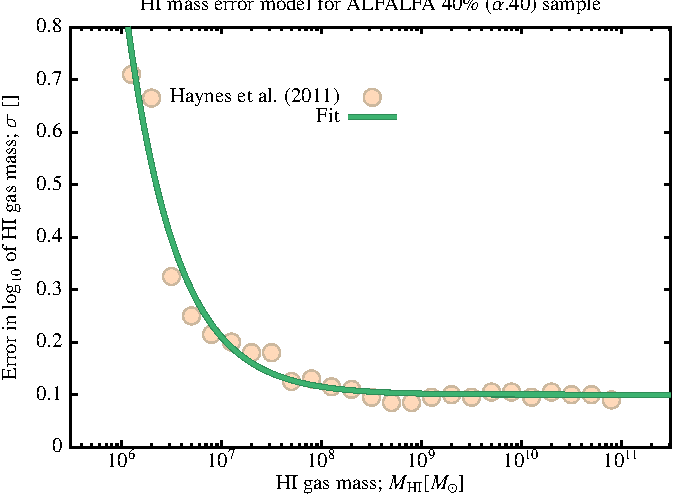
\includegraphics[width=85mm,trim=0mm 0mm 0mm 4mm,clip]{Plots/DataAnalysis/alfalfaHIMassErrorModel.pdf}
 \caption{The observational random error in galaxy HI mass as a function of HI mass for the ALFALFA survey. Points show the errors reported by \protect\cite{haynes_arecibo_2011}, while the line shows a simple functional form fit to these errors.}
 \end{center}
 \label{fig:ALFALFAErrorModel}
\end{figure}

In addition, we expect there to be significant scatter in the H$_2$/HI mass ratio at fixed total gas mass. For example, Figure~5 of \cite{power_redshift_2010} shows a broad distribution of such values. We approximate this scatter as a Gaussian random process with standard deviation $\sigma$. This random ``error'' is added in quadrature to the observational errors when constructing the mass function. For a prior on $\sigma$ we adopt a normal distribution with mean of $0.4$ (estimated from Figure~5 of \cite{power_redshift_2010}) and standard deviation $0.3$.

The model masses are then used to construct a mass function by binning into a histogram using the masses reported by \cite{martin_arecibo_2010} (modified as described above) as the centers of the bins (with bin boundaries placed at the geometric means of consecutive bin centers).

If the {\tt --modelDiscrepancies} option is given, then any multiplicative or additive discrepancies found are applied to the model mass function, and any additional covariance is added to the covariance matrix.

The covariance matrix is computed as
\begin{equation}
 {\bf C} = {\bf C}_{\rm obs} + {\bf C}_{\rm model,random} + \sum_i {\bf C}_{{\rm discrepancy}, i},
\end{equation}
where ${\bf C}_{\rm obs}$ is the covariance matrix of the observational data, ${\bf C}_{\rm model,random}$ is the covariance matrix of the model arising from random noise (due to the finite number of trees simulated, and ${\bf C}_{{\rm discrepancy}, i}$ is the covariance due to the $i^{\rm th}$ model discrepancy.

To construct ${\bf C}_{\rm model,random}$ we make use of the fact that \glc\ works by sampling a set of tree ``root masses'' from the $z=0$ dark matter halo mass function. From each root, a tree is grown, within which the physics of galaxy formation is then solved. Root masses are sampled uniformly from the halo mass function. That is, the cumulative halo mass function, $N(M)$, is constructed between the maximum and minimum halo masses to be simulated. The number of root masses, $N_{\rm r}$, to be used in a model evaluation is then determined. Root masses are then chosen such that
\begin{equation}
 N(M_i) = N(M_{\rm min}) {i-1 \over N_{\rm r}-1}
\end{equation}
for $i=1\ldots N_{\rm r}$ (noting that $N(M_{\rm max})=0$ by construction). 

Consider first those galaxies which form in the main branch of each tree (i.e. those galaxies which are destined to become the central galaxy of the $z=0$ halo). Suppose that we simulate $N_k$ halos of root mass $M_k$ at $z=0$. In such halos the main branch galaxies will, at any time, have stellar masses drawn from some distribution $p_k(M_\star|t)$. The number of such galaxies contributing to bin $i$ of the mass function is therefore binomially distributed with success probability $p_{ik} = \int_{M_{i,\rm min}}^{M_{i,\rm max}} p_k(M_\star|t) \d M_\star$ and a sample size of $N_k$. The contribution to the covariance matrix from these main branch galaxies is therefore:
\begin{equation}
 \mathcal{C}_{ij} = \left\{ \begin{array}{ll} p_{ik}(1-p_{ik}) N_k w_k^2 & \hbox{ if } i = j \\ -p_{ik} p_{jk} N_k w_k^2 & \hbox{ otherwise,} \end{array} \right.
\end{equation}
where $w_k$ is the weight to be assigned to each tree. To compute this covariance requires knowledge of the probabilities, $p_{ik}$. We estimate these directly from the model. To do this, we bin trees into narrow bins of root mass and assume that $p_{ik}$ does not vary significantly across the mass range of each bin. Using all realizations of trees that fall within a given bin, $k$, we can directly estimate $p_{ik}$.

In addition to the main branch galaxies, each tree will contain a number of other galaxies (these will be ``satellite'' galaxies at $z=0$, but at higher redshifts may still be central galaxies in their own halos). Tests have established that the number of satellites in halos is well described by a Poisson process. Note that each galaxy contributes Gaussian distribution to the mass function due to modelling of random errors in stellar mass determinations. For main branch galaxies this is simply accounted for when accumulating the probabilities, $p_{ik}$. For satellite galaxies, off-diagonal contributions to the covariance matrix arise as a result, $C_{ij} = w_k f_i f_j$, where $f_i$ is the fraction of the galaxy contributing to bin $i$ of the mass function.

The model likelihood is then computed using:
\begin{equation}
 \mathcal{L} = {1 \over \sqrt{(2 \pi)^n |{\bf C}|}} \exp\left[ -{1\over 2} \Delta {\bf C}^{-1} \Delta \right],
\end{equation}
where $\Delta_i = \Phi_{{\rm model}, i} - \Phi_{{\rm observed}, i}$ is the difference between the model and observed mass functions, and $n$ is the number of points in the mass function histogram.

Computing the large-scale structure contribution to the covariance function requires integration of the non-linear matter power spectrum over the Fourier transform of the survey window function. We use the method of \cite{peacock_non-linear_1996} to determine the non-linear matter power spectrum, because of its simplicity and speed. We have checked that using a more accurate non-linear matter power spectrum (e.g. \citealt{lawrence_coyote_2010}) makes negligible difference to our results.

To find a suitable \gls{hod} to describe the galaxies in the \cite{martin_arecibo_2010} sample we adopt the model of \cite{behroozi_comprehensive_2010}. This is an 11 parameter model which describes separately the numbers of satellite and central galaxies occupying a halo of given mass---the reader is referred to \cite{behroozi_comprehensive_2010} for a complete description of the functional form of this parametric \gls{hod}. 

To reproduce the mass function of \cite{martin_arecibo_2010} using this \gls{hod} we use the \gls{bie} \citep{weinberg_computational_2012} to constrain the \gls{hod} parameters. We use a likelihood
\begin{equation}
 \ln \mathcal{L} = -{1\over 2} \Delta\cdot \mathcal{C}^{-1}\cdot \Delta^{\rm T} - {N \over 2} \ln(2\pi) - {\ln |\mathcal{C}| \over 2},
\end{equation}
where $N$ is the number of bins in the mass function, $\mathcal{C}$ is the covariance matrix of the observed mass function, and $\Delta_i = \phi_i^{\rm (HOD)} - \phi_i^{\rm (observed)}$. Of course, it is precisely this covariance matrix, $\mathcal{C}$, that we are trying to compute. We therefore adopt an iterative approach as follows:
\begin{enumerate}
 \item make an initial estimate of the covariance matrix, assuming that only Poisson errors contribute (the covariance matrix is therefore diagonal, and the terms are easily computed from the measured mass function and the survey volume as a function of stellar mass);
 \item find the maximum likelihood parameters of the \gls{hod} given the observed mass function and the current estimate of the covariance matrix;
 \item using this \gls{hod} and the framework of \cite{smith_how_2012}, compute a new estimate of the covariance matrix, including all three contributions;
 \item repeat steps 2 and 3 until convergence in the covariance matrix is achieved.
\end{enumerate}
In practice we find that this procedure leads to an \gls{hod} and covariance matrix which oscillate between two states in successive iterations. The differences in the covariance matrix are relatively small however, so we choose to conservatively adopt the covariance matrix with the larger values. In future, adding additional constraints to the \gls{hod} (as described below) should help mitigate this problem.

\subsubsection{Shen et al. (2003) Late-Type Galaxy Size Distribution}\label{sec:SDSSLateTypeGalaxySizeDistribution}

This constraint utilizes the distribution of Petrosian half-light radii for $z\approx 0.07$ late-type galaxies measured by \cite{shen_size_2003} from the \gls{sdss}. The size function reported by \cite{shen_size_2003} is converted to the appropriate cosmology for the given \glc\ model (assuming that sizes scale as the angular diameter distance, and masses as the square of the luminosity distance).

Given a \glc\ model, total stellar masses of model galaxies are adjusted using:
\begin{equation}
 M_\star \rightarrow {\bf G} {\bf S} M_\star 
\end{equation}
where the ${\bf S}$ operator is a multiplicative factor accounting for systematic errors in stellar mass determination and is equal to \citep{behroozi_comprehensive_2010}
\begin{equation}
 \log_{\rm 10} S = \mu + \kappa \log_{\rm 10} \left({M_\star \over 10^{11.0}M_\odot}\right)
\end{equation}
where $\mu=${\tt [diskGalaxySizesSDSSZ0.07MassSystematic0]}, $\kappa=${\tt [diskGalaxySizesSDSSZ0.07MassSystematic1]}, and the {\bf G} operator is a multiplicative factor drawn from a log-normal distribution of width $0.0806$~dex for each galaxy to mimic the effects of random errors on stellar masses (motivated by the statement from \cite{shen_size_2003} who quote the 95\% confidence
interval on masses as being $\pm 40$\%).

{\bf Note:} This analysis currently assumes that model galaxies have disk Petrosian half-mass radii of
\begin{equation}
 R_{\rm 50} = 1.6676 {1 \over \sqrt{2}} \lambda R_{\rm vir}.
\end{equation}

Disk sizes of model galaxies are then adjusted using:
\begin{equation}
 R_{50} \rightarrow {\bf G} {\bf S} R_{50} 
\end{equation}
where the ${\bf S}$ operator is a multiplicative factor accounting for systematic errors in radius determination and in determination of radius from halo virial radius and spin and is equal to
\begin{equation}
 \log_{\rm 10} S = \mu + \kappa \log_{\rm 10} \left({R_{50} \over 1 \hbox{kpc}}\right)
\end{equation}
where $\mu=${\tt [iskGalaxySizesSDSSZ0.07RadiusSystematic0]}, $\kappa=${\tt [iskGalaxySizesSDSSZ0.07RadiusSystematic1]}, and the {\bf G} operator is a multiplicative factor drawn from a log-normal distribution of width $0.0128$~dex for each galaxy to mimic the effects of random errors on disk radii (estimated from the fractional errors reported in the \gls{sdss} database).

The model sizes and masses are then used to construct a mass-dependent radius function by binning into a 2-D histogram using the size and mass bins reported by \cite{shen_size_2003} (modified as described above) as the centers of the bins (with bin boundaries placed at the geometric means of consecutive bin centers).

If the {\tt --modelDiscrepancies} option is given, then any multiplicative or additive discrepancies found are applied to the model mass function, and any additional covariance is added to the covariance matrix.

The covariance matrix is computed as
\begin{equation}
 {\bf C} = {\bf C}_{\rm obs} + {\bf C}_{\rm model,random} + \sum_i {\bf C}_{{\rm discrepancy}, i},
\end{equation}
where ${\bf C}_{\rm obs}$ is the covariance matrix of the observational data, ${\bf C}_{\rm model,random}$ is the covariance matrix of the model arising from random noise (due to the finite number of trees simulated, and ${\bf C}_{{\rm discrepancy}, i}$ is the covariance due to the $i^{\rm th}$ model discrepancy.

The model covariance matrix is estimated using the sample methods as described in \S\ref{sec:AnalysisALFALFAHIMassFunction}. The only difference is that in this case we have a 2-D histogram. This 2-D histogram is ``flattened'' into a 1-D vector for purposes of likelihood computation however, so covariance matrix estimation proceeds unchanged. (Note that correlations between mass bins are accounted for, in additional to correlations between radius bins.) Since the radius functions of \cite{shen_size_2003} are normalized to unity at each mass, we must account for this in the covariance matrix. The radius function transforms as:
\begin{equation}
 f_{ik} \rightarrow {f_{ik} \over \Delta \log_{10} R \sum_i f_{ik} },
\end{equation}
where $i$ indexes radius bins, $k$ indexes mass bins, and $\Delta \log_{10} R$ is the width of the radius bin. The Jacobian of this transformation is simply
\begin{equation}
 J_{ij} = {\delta_{ij} - f_i \over  \Delta \log_{10} R \sum_i f_{ik}}.
\end{equation}
Therefore, the covariance matrix is modified according to $\mathcal{C} \rightarrow J \mathcal{C} J^{\rm T}$. The same transformation is applied to the covariance matrix of the observed data (for which the reported errors are simply the Poisson errors on each bin).

The model likelihood is then computed using:
\begin{equation}
 \mathcal{L} = {1 \over \sqrt{(2 \pi)^n |{\bf C}|}} \exp\left[ -{1\over 2} \Delta {\bf C}^{-1} \Delta \right],
\end{equation}
where $\Delta_i = \Phi_{{\rm model}, i} - \Phi_{{\rm observed}, i}$ is the difference between the model and observed mass functions, and $n$ is the number of points in the mass function histogram.

\section{Constraint Compilations}

To specify which constraints will be applied to a particular model, a compilation file is used. These must be stored in {\tt constraints/compilations}. An example of such a file follows:
\begin{verbatim}
<constraintCompilation>
  <constraint>
    <definition>constraints/constraints/stellarMassFunction_SDSS_z0.07.xml</definition>
    <weight>1.0</weight>
  </constraint>
  <constraint>
    <definition>constraints/constraints/hiMassFunction_ALFALFA_z0.00.xml</definition>
    <weight>1.0</weight>
  </constraint>
</constraintCompilation>
\end{verbatim}
Each {\tt constraint} element specifies one constraint that will be included in this compilation, and must contain a {\tt definition} element, giving the path of the configuration file for this constraint, and a {\tt weight} element which allows the relative weight given to each constraint to be varied\footnote{Note that, if your constraints are computing correct likelihoods, re-weighting them may not be a good idea. \emph{Caveat constrainor.}}.

\section{Constraint File}

\glc\ has a complete constraints infrastructure which implements various \gls{mcmc} algorithms to analyze the posterior probability distribution of the model given some compilation of constraints. The infrastructure is \gls{mpi} parallelized and ideal for running on large compute clusters.

To perform a constraint calculation simply build the constraint code:
\begin{verbatim}
 make Constrain_Galacticus.exe
\end{verbatim}
and run with a parameter file and configuration file. Typically, you will want to run this code under \gls{mpi}, for example:
\begin{verbatim}
 mpirun -n 4 Constrain_Galacticus.exe mcmcParameters.xml mcmcConfig.xml
\end{verbatim}
would run 4 processes (typically you will need to run many more than this). If running on a \gls{pbs} queue, embed this command in a suitable \gls{pbs} script and submit. 

The parameter file follows the same format as a standard \glc\ parameter file and specifies the values of parameters to be used. For example, the seed used fo pseudo-random number sequences can be specified in this file. 

The configuration file specifies the details of the constraint simulation to be performed. An example configuration file is:
\begin{verbatim}
<?xml version="1.0" encoding="UTF-8"?>
<simulationConfig>

  <likelihood>
    <type>Galacticus</type>
    <name>verySimplisticToStellarMassFunction</name>
    <compilation>stellarMassFunction_SDSS_z0.07.xml</compilation>
    <baseParameters>./mcmcWork/verySimplisticToStellarMassFunctionBase.xml</baseParameters>
    <workDirectory>./mcmcWork</workDirectory>
    <scratchDirectory>./mcmcScratch</scratchDirectory>
    <report>no</report>
    <randomize>no</randomize>
    <threads>4</threads>
    <saveState>no</saveState>
    <cpulimit>1200</cpulimit>
    <memoryLimit>2gb</memoryLimit>
    <environment>LD_LIBRARY_PATH=/opt/gcc-trunk/lib:/opt/gcc-trunk/lib64:/usr/local/upstream/lib:$LD_LIBRARY_PATH</environment>
    <environment>PATH=/opt/gcc-trunk/bin:$PATH</environment>
    <environment>GFORTRAN_ERROR_DUMPCORE=NO</environment>
  </likelihood>

  <convergence>
    <type>GelmanRubin</type>
    <Rhat>1.2</Rhat>
    <burnCount>100</burnCount>
    <testCount>100</testCount>
    <outlierCountMaximum>0</outlierCountMaximum>
    <outlierSignificance>0.95</outlierSignificance>
    <outlierLogLikelihoodOffset>60</outlierLogLikelihoodOffset>
  </convergence>
  
  <state>
    <type>history</type>
    <acceptedStateCount>100</acceptedStateCount>
  </state>
  
  <proposalSize>
    <type>adaptive</type>
    <gammaInitial>1.77</gammaInitial>
    <gammaFactor>1.414</gammaFactor>
    <acceptanceRateMinimum>0.4</acceptanceRateMinimum>
    <acceptanceRateMaximum>0.6</acceptanceRateMaximum>
    <updateCount>10</updateCount>
  </proposalSize>
  
  <randomJump>
    <type>adaptive</type>
  </randomJump>
  
  <simulation>
    <type>temperedDifferentialEvolution</type>
    <stepsMaximum>1000000</stepsMaximum>
    <stepsPostConvergence>100000</stepsPostConvergence>
    <acceptanceAverageCount>100</acceptanceAverageCount>
    <logFileRoot>./mcmcWork/mcmc/chains</logFileRoot>
    <temperatureMaximum>64.0</temperatureMaximum>
    <untemperedStepCount>20</untemperedStepCount>
    <temperedLevels>10</temperedLevels>
    <stepsPerLevel>10</stepsPerLevel>
  </simulation>

  <parameters>
    <parameter>
      <name>starFormationTimescaleDisksHaloScalingVirialVelocityExponent</name>
      <prior>
	<distribution>
	  <type>uniform</type>
	  <minimum>-6.0</minimum>
	  <maximum>+0.0</maximum>
	</distribution>
      </prior>
      <random>
	<type>Cauchy</type>
	<median>0.0</median>
	<scale>0.006</scale>
      </random>
    </parameter>
    <parameter>
      <name>starFormationTimescaleDisksHaloScalingRedshiftExponent</name>
      <prior>
	<distribution>
	  <type>uniform</type>
	  <minimum>-1.0</minimum>
	  <maximum>+4.0</maximum>
	</distribution> 
      </prior>
      <random>
	<type>Cauchy</type>
	<median>0.0</median>
	<scale>0.005</scale>
      </random>
    </parameter>
  </parameters>
  
</simulationConfig>
\end{verbatim}

The following subsections describe each entry in this file.

\subsection{{\tt likelihood}}

The {\tt likelihood} section specifies the likelihood function to be used in the simulation. The type of likelihood to use is specified by the {\tt type} element. The available choices are described in the following subsections.

\subsubsection{multivariateNormal}

The likelihood is a simple multivariate Gaussian, intended primarily for testing purposes. The distribution parameters are specified within the {\tt likelihood} element using:
\begin{verbatim}
  <mean>0.45 0.50</mean>
  <covariance>
    <row>1.0e-4 -0.9e-4</row>
    <row>-0.9e-4 1.0e-4</row>
  </covariance>
\end{verbatim}
where the {\tt mean} element gives the mean vector of $N$ elements, and the {\tt covariance} element contains $N$ {\tt row} elements each containing a vector of $N$ elements giving a single row of the covariance matrix. The likelihood is then:
\begin{equation}
\log \mathcal{L} = - {1 \over 2} \Delta \mathcal{C}^{-1} \Delta^{\rm T},
\end{equation}
where $Delta = \theta - \bar{\theta}$, $\theta$ is the state, $\bar{\theta}$ is the mean, and $\mathcal{C}$ is the covariance matrix.

\subsubsection{Galacticus}

The likelihood is computed by running and analyzing a \glc\ model. The details of the model to run are specified by the follow content within the {\tt likelihood} element:
\begin{verbatim}
  <name>verySimplisticToStellarMassFunction</name>
  <compilation>stellarMassFunction_SDSS_z0.07.xml</compilation>
  <baseParameters>./mcmcWork/verySimplisticToStellarMassFunctionBase.xml</baseParameters>
  <workDirectory>./mcmcWork</workDirectory>
  <scratchDirectory>./mcmcScratch</scratchDirectory>
  <report>no</report>
  <randomize>no</randomize>
  <threads>4</threads>
  <saveState>no</saveState>
  <cpulimit>1200</cpulimit>
  <memoryLimit>2gb</memoryLimit>
  <environment>LD_LIBRARY_PATH=/opt/gcc-trunk/lib:/opt/gcc-trunk/lib64:/usr/local/upstream/lib:$LD_LIBRARY_PATH</environment>
  <environment>PATH=/opt/gcc-trunk/bin:$PATH</environment>
  <environment>GFORTRAN_ERROR_DUMPCORE=NO</environment>
\end{verbatim}

The entries have the following meanings:
\begin{description}
\item[{\tt name}] A name to use for this calculation. It will be used as the name for jobs submitted to the PBS queue for example.
\item[{\tt compilation}] Specifies the compilation file to be used for this analysis.
\item[{\tt baseParameters}] Specifies the path to a \glc\ parameter file which will be used as the base set of parameter on top of which any parameter variations will be applied.
\item[{\tt workDirectory}] The full path to a directory in which the results (e.g. \gls{mcmc} chains) will be stored.
\item[{\tt scratchDirectory}] The full path to a scratch directory where \glc\ model outputs and other temporary data will be written.
\item[{\tt report}] If set to {\tt yes}, reports additional debugging information during the run.
\item[{\tt randomize}] If {\tt yes} then each model evaluation will be performed with a different random number seed. Otherwise, the same seed is used in all cases. Experiment shows that changing the random number seed between evaluations can seriously limit the ability of \gls{mcmc} algorithms to converge.
\item[{\tt threads}] The number of parallel OpenMP threads to use for each \glc\ model. It is recommended that this be set to the number of available cores on each node, and semaphoring (see \S{sec:Semaphores}) be used. In this way, each copy of \glc\ on a node will share resources, but as one instance finishes, the others will be able to make use of the freed resources.
\item[{\tt saveState}] If {\tt yes} then \glc\ will save its internal state prior to beginning evolution of each merger tree. This is intended for debugging purposes and so should normally be set to {\tt no}.
\item[{\tt cpulimit}] A CPU time limit for each model evalulation. This can be useful if certain obscure regions of the surveyed parameter space result in unacceptably long run times. Models will be killed after this time and a very low likelihood returned.
\item[{\tt environment}] One of more such element can appear. Each specifies the value of an environment variable to be set prior to launching the \glc\ model.
\item[{\tt storeResults}] If {\tt yes} then the full results (e.g. the quantities computed to compare with observational data) from each model evalulation will be stored. Otherwise, they are discarded after each evalulation. Use {\tt yes} with caution---a typical run might include millions of model evaluations which can quickly lead to huge amounts of data being written to disk.
\end{description}

\subsection{{\tt convergence}}

The {\tt convergence} section specifies the criterion to be used to judge when the simulation has converged. The type of convergence criterion to use is specified by the {\tt type} element. The available choices are described in the following subsections.

\subsubsection{{\tt never}}

This option assumes that the simulation never converges, and so the calculation will run indefinitely. It is intended primarily for testing purposes.

\subsubsection{{\tt GelmanRubin}}

This option adopts the convergence criterion proposed by \citeauthor{gelman_a._inference_1992}~(\citeyear{gelman_a._inference_1992}; see also \citealt{brooks_general_1998}), which compares the variance in parameter values within chains to that between chains. Outlier detection is applied to the chains using a standard Grubb's outlier test. The behavior of this criterion is controlled by the following options which should be placed within the {\tt convergence} element:
\begin{description}
\item [{\tt Rhat}] The correlation coefficient, $\hat{R}$, value at which to declare convergence.
\item [{\tt burnCount}] Set number of steps to burn before applying the convergence test.
\item [{\tt testCount}] Set the number of steps between successive applications of the convergence test.
\item [{\tt outlierSignificance}] The significance level required in outlier detection.
\item [{\tt outlierLogLikelihoodOffset}] The offset in log-likelihood from the current maximum likelihood chain required for a chain to be declared to be an outlier.
\item [{\tt outlierCountMaximum}] The maximum number of outlier chains allowed.
\end{description}

\subsection{{\tt state}}

The {\tt state} section specifies the type of object used to record the state of the simulation. The type of state object to use is specified by the {\tt type} element. The available choices are described in the following subsections.

\subsubsection{{\tt simple}}

This type stores the current state but makes no attempt to record a history of the state and so cannot provide measures of the mean or variance of state over the simulation history. It does, however, maintain a running average of the state acceptance rate. The number of steps over which the acceptance rate should be computed is specified by the {\tt acceptedStateCount}.

\subsubsection{{\tt history}}

An extension of the {\tt simple} state, this type also records the mean and variance of each parameter over the history of the simulation.

\subsection{{\tt proposalSize}}

The {\tt proposalSize} section specifies the method to use when selecting the proposal size parameter, $\gamma$ (the fraction of the vector connecting to chain state to be used as the proposal for another chain), for use in differential evolution simulations. The proposal size algorithm to use is specified by the {\tt type} element. The available choices are described in the following subsections.

\subsubsection{{\tt fixed}}

This option uses a fixed $\gamma$ specified by the {\tt gamma} element.

\subsubsection{{\tt adaptive}}

This option adaptively changes $\gamma$ in an attempt to maintain the acceptance rate at an acceptable level. The algorithm is controlled by the following parameters (to be specified as elements within the {\tt proposalSize} element):
\begin{description}
\item[{\tt gammaInitial}] The initial value for $\gamma$.
\item[{\tt gammaFactor}] The multiplicative factor by which $\gamma$ should be increased or decreased if the acceptance rate is out of range.
\item[{\tt acceptanceRateMinimum}] The minimum acceptance rate to accept before reducing $\gamma$.
\item[{\tt acceptanceRateMaximum}] The maximum acceptance rate to accept before reducing $\gamma$.
\item[{\tt updateCount}] The number of steps between successive checks of the acceptance rate.
\end{description}

\subsection{{\tt randomJump}}

The {\tt randomJump} section specifies the method to use when adding a random jump component to proposals in differential evolution simulations. The random jump algorithm to use is specified by the {\tt type} element. The available choices are described in the following subsections.

\subsubsection{{\tt simple}}

The random jumps are drawn directly from the distributions specified in the {\tt random} element of each parameter (see \S\ref{sec:ParametersPriors}).

\subsubsection{{\tt adaptive}}

The random jumps are drawn from the distributions specified in the {\tt random} element of each parameter (see \S\ref{sec:ParametersPriors}) and then multiplied by the currently occupied range of each parameter (i.e. the maximum value of the parameter over all current chain states minus the minimum value of each parameter over all current chain states).

\subsection{{\tt simulation}}

The {\tt simulation} section specifies the algorithm to use to perform the simulation. The simulation algorithm to use is specified by the {\tt type} element. The available choices are described in the following subsections.

\subsubsection{{\tt differentialEvolution}}

This option uses the differential evolution algorithm of \cite{terr_braak_markov_2006}. Multiple, parallel chains are run and proposals are constructed by selecting two chains at random, taking a fraction, $\gamma$, of the vector connecting the two chain states and adding this to the state of the current chain. The details of the algorithm are controlled by the following elements which should be embedded within the {\tt simulation} element:
\begin{description}
\item[{\tt stepsMaximum}] The maximum number of steps to take.
\item[{\tt stepsPostConvergence}] The number of steps to perform after convergence is attained.
\item[{\tt acceptanceAverageCount}] The number of steps over which to average the acceptance rate.
\item[{\tt stateSwapCount}] The number of steps after which to set $\gamma=1$ to allow chains to swap states.
\item[{\tt logFileRoot}] The full path and root name of a file to log results to. The actual file name will have the rank of the \gls{mpi} process appended to it.
\end{description}

\subsubsection{{\tt temperedDifferentialEvolution}}

This option extends the {\tt differentialEvolution} option to include tempering during which the likelihood function is heated up and cooled down to allow chains to more easily walk through the likelihood landscape. In addition to the options for the {\tt differentialEvolution} algorithm, the details of the algorithm are controlled by the following elements whichy should be embedded within the {\tt simulation} element:
\begin{description}
\item[{\tt untemperedStepCount}] The number of untempered (i.e. $T=1$) steps to take between tempering cycles.
\item[{\tt temperatureMaximum}] The maximum temperature to use when tempering.
\item[{\tt temperedLevels}] The number of tempered levels to use.
\item[{\tt stepsPerLevel}] The number of differential evolution steps to take at each tempering level;
\item[{\tt gammaTemperatureExponent}] The exponent of the boost in $\gamma$ during tempered steps.
\end{description}

In each tempering cycle, the temperature is raised through levels $1$\ldots$N$ (where $N=${\tt temperedLevels}), and then back down through levels $N-1$\ldots$1$. The temperature at level $i$ is given by:
\begin{equation}
\log T_i = {i \over N} \log T_{\rm max},
\end{equation}
where $T_{\rm max}=${\tt temperatureMaximum}. During tempered steps, the $\gamma$ parameter of the differential evolution algorithm is increased by a factor $T^\alpha$, where $\alpha=${\tt gammaTemperatureExponent}. A value of $\alpha=1/2$ is optimal for a Gaussian likelihood.

\subsection{Parameters and Priors}\label{sec:ParametersPriors}

The {\tt parameters} section contains a list of all parameters to be varied in the analysis. Each parameter is described by one {\tt parameter} element. That element must contain a {\tt name} element, which gives the name of the parameter, a {\tt prior} element that contains a {\tt distribution} element defining the distribution for this prior, and (for differential evolution simulations) a {\tt random} element that defines the distribution to be used for the random perturbation to be added to this parameter in proposals.

\subsubsection{Loading External Parameters/Priors}

It is also possible to load parameters and their priors from external files. This is useful to add common sets of parameters, such as cosmological parameter. To do so, add an element of the form:
\begin{verbatim}
<xi:include href="../../constraints/parameters/wmap9Cosmology.xml" 
   xmlns:xi="http://www.w3.org/2001/XInclude" />
\end{verbatim}
\emph{after} the {\tt parameters} section of the constraint file. The {\tt href} attribute must give the path (relative to the constraint file, or absolute) to the external parameter file. This file should contain its own {\tt parameters} block, describing all parameters to be varied along with their priors. 

\subsubsection{Derived Parameter Values}

It is possible to define parameters in terms of other parameters. Common uses for this include:
\begin{itemize}
 \item Setting $\Omega_\Lambda$ from the value of $\Omega_{\rm M}$ to enforce a flat Universe;
 \item Setting the values of parameters with correlated priors as linear combinations of dummy parameters for which the priors are independent.
\end{itemize}
To define a parameter in this way include a {\tt parameter} element of the form:
\begin{verbatim}
<parameter>
 <name>sigma_8</name>
 <define>0.8178+%cosmology0*0.003817+%cosmology1*0.007931+%cosmology2*0.01002
    +%cosmology3*0.001584+%cosmology4*0.002931+%cosmology5*0.001727</define>
</parameter>
\end{verbatim}
Here the {\tt define} element gives an equation for the parameter in terms of other parameters. All standard mathematical operators and functions (as recognized by Perl) can be used, and other parameters referenced by using their name prefixed with a ``\%''.

\subsubsection{Including External Parameters}

Predefined sets of parameters (along with their priors) can be included using the {\tt xi:include} element. For example,
\begin{verbatim}
 <xi:include href="../../constraints/parameters/wmap7Cosmology.xml"
    xmlns:xi="http://www.w3.org/2001/XInclude" />
\end{verbatim}
will include a set of parameters from the file {\tt ../../constraints/parameters/wmap7Cosmology.xml} which defines priors on cosmological parameters consistent with the covariance matrix of the WMAP-7 cosmological constraints \citep{komatsu_seven-year_2010}.

\subsection{Distributions}

Various distribution functions (for priors and random perturbations) are supported. Where needed, the type of distribution should be specified in a {\tt type} element. Additional parameters of the distribution are specified using the elements described in the following subsections.

\subsubsection{{\tt uniform}}

A uniform distribution over a finite range
\begin{equation}
P(x) \propto \left\{ \begin{array}{ll} 1 & \hbox{ if } x_{\rm l} \leq x \leq x_{\rm u} \\ 0 & \hbox{ otherwise.}  \end{array} \right.
\end{equation}
Specified using:
\begin{description}
\item[{\tt minimum}] The lower limit of the range, $x_{\rm l}$;
\item[{\tt maximum}] The upper limit of the range, $x_{\rm u}$.
\end{description}

\subsubsection{{\tt logUniform}}

A distribution uniform in the logarithm of $x$ over a finite range
\begin{equation}
P(x) \propto \left\{ \begin{array}{ll} x^{-1} & \hbox{ if } x_{\rm l} \leq x \leq x_{\rm u} \\ 0 & \hbox{ otherwise.}  \end{array} \right.
\end{equation}
Specified using:
\begin{description}
\item[{\tt minimum}] The lower limit of the range, $x_{\rm l}$;
\item[{\tt maximum}] The upper limit of the range, $x_{\rm u}$.
\end{description}

\subsubsection{{\tt normal}}

A normal distribution, optionally with lower and upper limits:
\begin{equation}
P(x) \propto \left\{ \begin{array}{ll} \exp[-(x-\mu)^2/2S] & \hbox{ if } x_{\rm l} \leq x \leq x_{\rm u} \\ 0 & \hbox{ otherwise.}  \end{array} \right.
\end{equation}
Specified using:
\begin{description}
\item[{\tt mean}] The mean, $\mu$;
\item[{\tt variance}] The variance, $S$;
\item[{\tt minimum}] The lower limit of the range, $x_{\rm l}$;
\item[{\tt maximum}] The upper limit of the range, $x_{\rm u}$.
\end{description}

\subsubsection{{\tt Cauchy}}

A Cauchy distribution:
\begin{equation}
P(x) \propto \left[1+{x-x_0\over\gamma}\right]^{-1}.
\end{equation}
Specified using:
\begin{description}
\item[{\tt median}] The median, $x_0$;
\item[{\tt scale}] The scale, $\gamma$;
\end{description}

\subsubsection{{\tt StudentT}}

Student's t-distribution:
\begin{equation}
P(x) \propto \left(1 + {x^2\over \nu}\right)^{-(\nu+1)/2}
\end{equation}
Specified using:
\begin{description}
\item[{\tt degreesOfFreedom}] The number of degrees of freedom, $\nu$.
\end{description}


\backmatter

\chapter{Acknowledgements}

In addition to the tools and libraries required to compile and run \glc, development of \glc\ has benefitted from extensive use of the following: \href{http://www.gnu.org/software/octave/}{{\sc GNU Octave}}, \href{http://maxima.sourceforge.net/}{{\sc Maxima}}, \href{http://edu.kde.org/cantor/}{{\sc Cantor}}, \href{http://kile.sourceforge.net/}{{\sc Kile}}, \href{http://www.gnu.org/software/emacs/}{{\sc Emacs}} and \href{http://valgrind.org/}{{\sc Valgrind}}. We are grateful to the members of the {\sc GNU Fortran} mailing list for invaluable discussions and fixes for compiler problems. We thank John Burkardt for making available the {\sc Bivar} algorithm for performing interpolation on data irregularly spaced on a 2D plane and Dima Verner for making available codes to compute various atomic data for astrophysics. Chris Power provided instructions for installing \glc\ under Mac OS X. The community of \glc\ users\footnote{In particular, Christoph Behrens, Jianling Gan, Markus Haider, Harald H\"oller, Eve Kovacs, Ting-Wen Lan, Adrian Pope, Luiz Felippe Rodrigues, Sergio Sanes, Martin White and Liyan Xu.} have provided invaluable feedback and bug reports. Gian Luigi Granato and Laura Silva kindly provided modifications to their \href{http://adlibitum.oat.ts.astro.it/silva/grasil/grasil.html}{\sc Grasil} code to allow it to read \glc\ outputs.


\bibliographystyle{plainnat}
\bibliography{GalacticusAccented}

\printglossaries

\citeindextrue
\printindex

\end{document}
